\documentclass{article} % For LaTeX2e
\usepackage[preprint]{colm2026_conference}

\usepackage{microtype}
\usepackage{hyperref}
\usepackage{url}
\usepackage{booktabs}
\usepackage{lineno}
\usepackage{amsmath,amsfonts,amssymb}
\usepackage{tikz}
\usetikzlibrary{trees, shapes.geometric, arrows.meta, positioning, calc, shadows, backgrounds, fit}
\usepackage[edges]{forest}
\usepackage{enumitem}
\usepackage{multirow}
\usepackage{graphicx}
\usepackage{placeins}
\usepackage{fontawesome}

% === Figure fonts and colors (shared by inline TikZ figures) ===
\usepackage{tgheros}
\usepackage{sansmath}
\definecolor{deepblue}{HTML}{1A5276}
\definecolor{midblue}{HTML}{2980B9}
\definecolor{lightblue}{HTML}{AED6F1}
\definecolor{lightblue2}{HTML}{D4E6F1}
\definecolor{deeppurple}{HTML}{6C3483}
\definecolor{deepgray}{HTML}{2C3E50}
\definecolor{midpurple}{HTML}{8E44AD}
\definecolor{lightpurple}{HTML}{D2B4DE}
\definecolor{deeporange}{HTML}{B9470B}
\definecolor{midorange}{HTML}{E67E22}
\definecolor{lightorange}{HTML}{F5CBA7}
\definecolor{coralpink}{HTML}{E74C3C}
\definecolor{midgray}{HTML}{7F8C8D}
\definecolor{panelbg}{HTML}{F5F8FC}
\definecolor{darkblue}{rgb}{0, 0, 0.5}
\hypersetup{colorlinks=true, citecolor=darkblue, linkcolor=darkblue, urlcolor=darkblue}

\title{A Survey of On-Policy Distillation for Large Language Models}

\author{Mingyang Song \& Mao Zheng \\
Large Language Model Department \\Tencent, China\\
\texttt{nickmysong@tencent.com}\\[2pt]
\faGithub\ \href{https://github.com/nick7nlp/Awesome-LLM-On-Policy-Distillation}{nick7nlp/Awesome-LLM-On-Policy-Distillation}}

\newcommand{\fix}{\marginpar{FIX}}
\newcommand{\new}{\marginpar{NEW}}

% Math macros
\newcommand{\E}{\mathbb{E}}
\newcommand{\KL}{D_{\mathrm{KL}}}
\newcommand{\ptheta}{p_\theta}
\newcommand{\pteacher}{p_T}
\newcommand{\pdata}{p_{\mathrm{data}}}
\newcommand{\loss}{\mathcal{L}}
\DeclareMathOperator*{\argmin}{arg\,min}
\DeclareMathOperator*{\argmax}{arg\,max}

\begin{document}
\maketitle

\begin{abstract}
As Large Language Models (LLMs) continue to grow in both capability and cost, transferring frontier capabilities into smaller, deployable students has become an important engineering problem, and knowledge distillation remains a common technique for this transfer. The prevailing recipe in industrial pipelines, static imitation of teacher-generated text, carries a structural weakness that grows more severe as tasks become longer and more reasoning-intensive. Because the student is trained on flawless teacher prefixes but generates its own at inference, small errors tend to accumulate into trajectories it has rarely been trained to recover from, and the resulting exposure bias has been shown to scale roughly with the square of sequence length. On-Policy Distillation (OPD) reorganizes the training loop around this observation by having the teacher provide feedback on what the student \emph{actually produces}, with the goal of reducing the compounding term toward linear and reframing distillation as an iterative correction process rather than single-pass imitation. The resulting literature has expanded along divergence design, reward-guided optimization, and self-play, yet contributions remain scattered across the knowledge distillation, RLHF, and imitation learning communities without a unified treatment. To our knowledge, this is the first survey dedicated to On-Policy Distillation for LLMs. We formalize OPD as $f$-divergence minimization over student-sampled trajectories, organize the field along three design axes (what to optimize, where the signal comes from, and how to stabilize training in practice), and consolidate success conditions, recurring failure modes, and the connection between OPD and KL-constrained reinforcement learning. We close with open problems that emerge from this synthesis, including distillation scaling laws, uncertainty-aware feedback, agent-level distillation, and the growing overlap between knowledge distillation and RL.
\end{abstract}

\section{Introduction}
\label{sec:intro}

The capability of Large Language Models (LLMs) has advanced rapidly over the past two years, with recent systems reaching strong reported performance on reasoning, code generation, and multilingual benchmarks~\citep{2505.09388,2501.12948,2408.00118}. This progress has come at a training cost that only a few organizations can sustain. Transferring the resulting capabilities from large frontier models into smaller deployable students has therefore become a core step in the modern LLM pipeline. Knowledge distillation, first formalized by \citet{1503.02531} as a way for a student to inherit the soft output structure of a teacher, has broadened in scope over this period. What began as a model compression technique for transferring knowledge within the same architecture now serves as a general mechanism for moving capabilities across model scales and architectural families. The release of DeepSeek-R1~\citep{2501.12948} made this shift concrete, distilling a 671B mixture-of-experts teacher into dense students spanning 1.5B to 70B parameters while preserving long chain-of-thought reasoning largely intact.

The dominant recipe behind these successes, however, has a known structural weakness. In almost all large-scale pipelines, distillation proceeds \emph{off-policy}. The student is trained to match the teacher's next-token distribution over a fixed corpus, typically the original pre-training data or traces generated in advance by the teacher, and every gradient step conditions on flawless teacher prefixes. At inference, this assumption no longer holds. The student generates autoregressively from its own partial outputs, and any divergence between the training states and the states it visits at deployment translates into compounding error along the trajectory. This corresponds to the \emph{compounding error} identified in interactive imitation learning~\citep{1011.0686}, where autoregressive generation amplifies the distribution mismatch quadratically in sequence length, producing an expected discrepancy of $O(\epsilon T^2)$ over a horizon $T$. The consequences are most pronounced on reasoning tasks, where a single early misstep can derail an entire proof or program. \citet{2305.15717} report that off-policy imitation of proprietary LLMs often yields students that reproduce surface style without acquiring the underlying reasoning competence.

Addressing this mismatch requires changing \emph{where} the training data comes from rather than \emph{what} is being matched. \textbf{On-Policy Distillation (OPD)} addresses this by shifting the sampling distribution from a static corpus to the student's own evolving policy. The student proposes trajectories, populates the states it will visit at deployment, and receives teacher feedback on those states rather than on idealized expert prefixes. Depending on the available teacher access, this feedback ranges from full token-level distributions in white-box settings~\citep{2306.13649,2306.08543}, through scalar rewards or pairwise preferences when only black-box APIs are available~\citep{2511.10643,2305.12870}, to contrastive signals the model derives from its own outputs in teacher-free settings~\citep{2601.18734}. The theoretical payoff mirrors the classical DAgger result~\citep{1011.0686}, where querying an expert on the learner's own visited states reduces the $O(\epsilon T^2)$ compounding of off-policy imitation to $O(\epsilon T)$. Translated into autoregressive language modeling, this turns distillation from a single-pass matching problem into an iterative optimization loop in which the training distribution co-evolves with the model, allowing distributional gaps between training and deployment to be corrected during training rather than deferred to inference.

The body of work that has emerged from this reformulation can be organized around a small number of recurring design choices. Early methods focused on \emph{how} to sample and \emph{which} divergence to apply on student trajectories~\citep{2306.13649,2306.08543,2402.03898}, establishing that an appropriate divergence depends on where in the sequence one is training and what kind of supervision the teacher can supply. A parallel line of work revealed that the resulting objective is formally equivalent to a KL-constrained form of reinforcement learning~\citep{2602.12125}, bridging two previously separate research communities. A third branch showed that the ``teacher'' need not be external at all, with methods such as OPSD~\citep{2601.18734} and SD-ZERO~\citep{2604.12002} showing that a model can bootstrap improvement from its own generations by exploiting asymmetries in its output distribution across contexts. These ideas have since moved from papers into production pipelines, with Qwen3~\citep{2505.09388}, DeepSeek-V4~\citep{deepseekv4}, Gemma~2~\citep{2408.00118}, and MiMo-V2-Flash~\citep{2601.02780} all adopting OPD as a core training ingredient. The adoption cuts across architectural lines, covering both mixture-of-experts and dense systems and spanning proprietary and open-weight release strategies, because all of these systems face the same structural problem once reasoning chains grow long enough for compounding error to dominate. DeepSeek-V4 went the furthest, replacing its mixed RL stage with pure multi-teacher OPD for model consolidation.

GKD~\citep{2306.13649}, alongside the concurrent MiniLLM~\citep{2306.08543}, brought on-policy distillation into the LLM era in mid-2023, and in less than two years the literature has expanded to over two hundred papers spanning divergence design, reward-guided optimization, self-play, multi-teacher debate, agentic trajectory distillation, and cross-modal transfer. The research focus has shifted accordingly. Where early work asked whether on-policy training helps at all, the current frontier asks how to make it efficient enough for trillion-parameter teacher inference, how to extend it beyond single-turn generation into multi-step agent trajectories, and how to unify it with the reinforcement learning pipelines that increasingly share its computational infrastructure. This trajectory parallels a broader shift in LLM development. As models become more capable and reasoning chains grow longer, the gap between off-policy training states and deployment-time states widens, which makes on-policy correction increasingly attractive for the next generation of reasoning-capable systems~\citep{2603.25562,deepseekv4}.

Despite this rapid adoption, the research literature on OPD has yet to catch up with the practice. Methods approach the same problem through the separate lenses of knowledge distillation, RLHF, and interactive imitation learning, each carrying different notations, benchmarks, and failure taxonomies from its parent community. Existing surveys of LLM distillation~\citep{2402.13116} generally retain the classical compression framing, treating off-policy and on-policy methods as interchangeable variants instead of as regimes with materially different theoretical guarantees and failure modes. As a result, no current treatment we are aware of offers a unified mathematical account of the on-policy dynamics that connect these threads, and a systematic comparison across the white-box, black-box, and teacher-free instantiations that researchers and engineers must now weigh against one another in practice remains missing.

This survey addresses that gap. To our knowledge, it is the first to treat on-policy distillation as a distinct paradigm rather than a variant of classical knowledge distillation, and it develops a unified account through four contributions that also structure the rest of the paper.
\begin{itemize}[leftmargin=1.5em]
    \item \textbf{A unified theoretical framework.} We recast the transition from off-policy to on-policy distillation as a sequential decision-making problem and show that the core OPD algorithms are instances of $f$-divergence minimization over student-sampled trajectories (Section~\ref{sec:background}). This framework supplies a common analytical vocabulary for methods previously studied in isolation and clarifies their relationships in terms of divergence choice, argument ordering, and sampling mixture.
    \item \textbf{A design-centric taxonomy.} Rather than grouping methods by surface similarity, we organize them along three core design axes (Section~\ref{sec:landscape}), namely objective function design (Section~\ref{sec:objectives}), signal source architecture (Section~\ref{sec:signal}), and training dynamics optimization (Section~\ref{sec:dynamics}). The resulting one-method-one-category classification clarifies the relationships among methods in terms of the specific design choices each paper optimizes.
    \item \textbf{A theoretical account of failure.} We consolidate the empirical record into a coherent view of when and why OPD breaks down (Section~\ref{sec:understanding}), covering the flawed prefix trap, self-play saturation, diversity collapse, the calibration-capability gap, and emerging multi-turn agentic failure modes, and we describe formal conditions under which OPD improves over off-policy alternatives.
    \item \textbf{Comprehensive coverage and comparative analysis.} We survey the white-box, black-box, and self-distillation regimes within this common framework, summarize them in per-section comparison tables (Tables~\ref{tab:method_comparison},~\ref{tab:methods_fixed_div}--\ref{tab:methods_efficiency}, and~\ref{tab:experimental_configs}), and document method selection factors (Section~\ref{subsec:decision_tree}) that map deployment constraints to applicable methods and compute budgets.
\end{itemize}

The structure of the paper follows the same design-axis logic. Section~\ref{sec:background} develops the mathematical preliminaries, formalizes autoregressive generation as a sequential decision problem, and derives the exposure bias that motivates on-policy training. Section~\ref{sec:landscape} presents the method landscape and selection considerations. Sections~\ref{sec:objectives}--\ref{sec:dynamics} then traverse the three design axes from ``what to optimize'' through ``where the signal comes from'' to ``how to stabilize training in practice,'' with each section building on the choices surfaced in the previous one. Section~\ref{sec:understanding} consolidates the theoretical perspectives, showing that the patterns observed across Sections~\ref{sec:objectives}--\ref{sec:dynamics} follow from a small number of unifying principles. Section~\ref{sec:applications} discusses industrial deployments, system-level optimization, and emerging domains, and Section~\ref{sec:future} lays out the open problems that emerge from this synthesis.

Our scope is centered on the on-policy regime. We cover methods in which the student generates its own training data during distillation, and we include work from adjacent fields such as imitation learning, online RL, and preference optimization whenever it operates on student-generated data under teacher or verifier supervision. We exclude generic off-policy KD, compression techniques orthogonal to the training regime such as pruning and quantization, and inference-time methods that leave model weights unchanged.

\section{Background and Unified Math}
\label{sec:background}

To understand why on-policy training is often preferable, we formalize the compounding geometry of autoregressive generation. We begin with classical KD and its limitations, then establish the unified $f$-divergence framework that subsumes modern OPD objectives.

\textbf{Defining ``on-policy.''} A distillation method is \emph{on-policy} if the training data for the student is sampled from the student's own current policy $\ptheta$ at training time, rather than from a fixed external corpus $\mathcal{D}$ or from the teacher's generation distribution $\pteacher$. Formally, on-policy training optimizes:
\begin{equation}
    \min_\theta \E_{x \sim \mathcal{D}}\, \E_{y \sim \ptheta(\cdot|x)} \left[ \mathcal{L}(y, x; \theta, T) \right]
\end{equation}
where $\mathcal{L}$ is the distillation loss (divergence, reward, or hybrid). The key distinction is that the \emph{outer} expectation is over the student's own generations, not a static dataset. This creates a non-stationary optimization landscape because as $\theta$ updates, the data distribution $\ptheta$ shifts, requiring fresh rollouts at each training step. The computational cost of this fresh generation is a central systems-level challenge of OPD (Section~\ref{subsec:compute}).

\textbf{Notation.} Throughout this survey, we use lowercase $p$ for token-level conditional distributions ($\pteacher(\cdot|x, y_{<t})$ for teacher, $\ptheta(\cdot|x, y_{<t})$ for student) and uppercase $P$ for sequence-level distributions ($P_T(y|x)$, $P_\theta(y|x)$). $\mathcal{D}$ denotes the training dataset, $\pdata$ the data distribution, and $|V|$ the vocabulary size. $\KL$ and $D_f$ denote KL divergence and general $f$-divergence respectively. In the RL formalization, $\pi$ denotes policies (e.g., $\pi_{\mathrm{mix}}$ for a mixture policy, $\pi_{\text{teach}}$ for a sequence-level teacher policy in DPO-style derivations, $\pi_{\text{ref}}$ for a reference policy) and $R(x,y)$ the outcome reward. When discussing individual methods, we follow each paper's conventions where clarity demands.

\subsection{Classical Knowledge Distillation}

The original KD formulation~\citep{1503.02531} trains the student to match the teacher's temperature-softened output distribution:
\begin{equation}
    p_T^{(\tau)}(y|x) = \frac{\exp(z_y / \tau)}{\sum_{j} \exp(z_j / \tau)}
\end{equation}
where $z_y$ are the teacher's logits and $\tau > 1$ is a temperature parameter. When $\tau \to \infty$, the softened distribution approaches a uniform distribution over the vocabulary, exposing the teacher's ``dark knowledge'' about inter-class similarities that hard labels hide. The gradient of the distillation loss with respect to the student's logits $z_i^{\mathcal{S}}$ shows why temperature matters:
\begin{equation}
    \frac{\partial \loss_{\text{KD}}}{\partial z_i^{\mathcal{S}}} = \frac{1}{\tau}(p_i^{\mathcal{S}} - p_i^{\mathcal{T}})
\end{equation}
In the high-temperature limit ($\tau \to \infty$), a Taylor expansion $\exp(z_i/\tau) \approx 1 + z_i/\tau$ together with the zero-mean assumption $\sum_i z_i^{\mathcal{S}} = \sum_i z_i^{\mathcal{T}} = 0$ reduces the gradient to $\frac{1}{|V|\tau^2}(z_i^{\mathcal{S}} - z_i^{\mathcal{T}})$~\citep{1503.02531}, so classical KD in this regime is equivalent to minimizing the mean squared error between raw logits. This encourages the student to replicate the teacher's \emph{entire} logit structure, transferring both primary predictive modes and nuanced sub-optimal probability masses (the ``dark knowledge''). The $1/\tau^2$ factor explains why the soft-target term is commonly upweighted by $\tau^2$ relative to the hard-label cross-entropy in the combined KD objective. In practice, LLM distillation operates at $\tau = 1$ or low-to-moderate temperatures~\citep{2402.11890} because the large vocabulary ($|V| > 30{,}000$) already produces richly structured non-peak probabilities without explicit softening, and higher temperatures may amplify noise in the teacher's poorly calibrated tail distribution.

For autoregressive LLMs, the token-level distillation loss factors as:
\begin{equation}
    \loss_{\text{Token-KD}} = \E_{x, y \sim \mathcal{D}} \left[ \sum_{t=1}^{|y|} \KL(\pteacher(\cdot | x, y_{<t}) \parallel \ptheta(\cdot | x, y_{<t})) \right]
\end{equation}
This is computationally tractable because it relies on static, pre-computed prefixes from the dataset, but it optimizes next-token accuracy while assuming an error-free history $y_{<t}$. \citet{1606.07947} extended this to Sequence-Level Knowledge Distillation (Seq-KD), which instead minimizes the global KL divergence over the entire sequence space:
\begin{equation}
    \loss_{\text{Seq-KD}} = \KL(P_T(y|x) \parallel P_\theta(y|x)) = \sum_{y \in \mathcal{Y}} P_T(y|x) \log \frac{P_T(y|x)}{P_\theta(y|x)}
\end{equation}
Since $|\mathcal{Y}| = |V|^T$ grows exponentially with length, exact computation is intractable. Seq-KD approximates $P_T(y|x)$ with a Dirac delta at the beam-search output $\hat{y} = \arg\max_y P_T(y|x)$, reducing to standard negative log-likelihood on teacher-generated sequences:
\begin{equation}
    \loss_{\text{Seq-KD}} \approx -\log P_\theta(\hat{y}|x)
\end{equation}
This approximation works well when the teacher is highly confident but discards much of the information about the teacher's uncertainty and alternative modes. The practical consequence is twofold. Seq-KD collapses the teacher's distributional richness into a single point estimate, and it still trains on a \emph{static} dataset disconnected from the student's own generation behavior. These two limitations (loss of distributional signal and off-policy training) motivate the richer objectives below.

Subsequent work~\citep{2402.11890} revisited these foundations for modern LLMs and suggested that classical assumptions (small teacher-student gap, shared vocabulary, similar architectural inductive biases) frequently fail when distilling across heterogeneous model families. The gap between classical assumptions and modern reality motivates the more general $f$-divergence framework below.

\textbf{From classical KD to on-policy.} The historical progression from Hinton's classical KD to modern OPD amounts to a series of relaxations of four classical assumptions, namely (1)~shared vocabulary, (2)~i.i.d.\ data, (3)~static teacher, and (4)~off-policy training data. Seq-KD~\citep{1606.07947} relaxes assumption (2) by operating at the sequence level but retains the static data assumption. GKD~\citep{2306.13649} relaxes assumption (4) by training on student-generated sequences. DSKD~\citep{2504.11426} relaxes assumption (1) through dual-space alignment. G-OPD~\citep{2602.12125} relaxes assumptions (2)--(4) simultaneously while adding RL-augmented reward extrapolation that pushes the student beyond the teacher's frontier. Each relaxation targets a specific failure mode that intensifies with model scale. Vocabulary mismatch is often irrelevant for same-family distillation but severe for cross-family transfer (relaxation~1), while exposure bias is negligible for short sequences but highly problematic for multi-step reasoning (relaxation~4). This progression is not merely historical but informative, since the relevant assumptions in a given deployment scenario determine which level of relaxation is necessary, and unnecessary relaxation introduces avoidable complexity.

\subsection{Off-Policy Exposure Bias}

The token-level loss in Eq.~(4) conditions on ground-truth prefixes $y_{<t}$ drawn from a static dataset. During inference, the student generates its own prefixes, creating a distribution mismatch between training and deployment that compounds over sequence length. We now formalize why this mismatch is catastrophic.

Standard knowledge distillation minimizes the KL divergence over states drawn from the dataset distribution $d_{\mathcal{D}}(s)$:
\begin{equation}
    \loss_{\mathrm{Off-Policy}} = \E_{x, y \sim \pdata} \left[ \sum_{t=1}^{|y|} \KL(\pteacher(\cdot | x, y_{<t}) \parallel \ptheta(\cdot | x, y_{<t})) \right]
\end{equation}
At inference, the student acts according to its own policy, inducing a different state visitation distribution $d_{\pi_\theta}(s)$. By the DAgger theorem~\citep{1011.0686}, if a policy mimics an expert with per-step error $\epsilon$ under the training distribution, the expected total discrepancy over a trajectory of length $T$ under the learner's own state visitation scales as $O(\epsilon T^2)$.

This quadratic compounding has severe practical consequences for reasoning tasks. Even under the simplest independent-error assumption, a mathematical proof requiring 10 reasoning steps with per-step accuracy 95\% yields only $(0.95)^{10} \approx 60\%$ trajectory-level correctness. The DAgger bound predicts something strictly worse. Because off-policy training rarely exposes the student to its own error states, each mistake pushes the model into regions where its next-step accuracy degrades further (distributional shift), producing $O(\epsilon T^2)$ total error rather than the $O(\epsilon T)$ of independent compounding. On-policy training offers a way to mitigate this vicious cycle by exposing the student to its own error states during training, so that it can learn recovery strategies that keep distributional drift from amplifying local mistakes into trajectory-level collapse.

\textbf{Remark on the DAgger bound in LLMs.} While the theoretical reduction from $O(\epsilon T^2)$ to $O(\epsilon T)$ is appealing, applying the DAgger bound to LLMs demands careful qualification. The original theorem assumes an \emph{interactive expert} that emits optimal actions in any state. In white-box OPD, the ``expert'' emits a next-token distribution $\pteacher(y_t | \hat{y}_{<t})$ conditioned on the student's prefix $\hat{y}_{<t}$. If the student hallucinates a severely out-of-distribution prefix, the teacher's conditional distribution may itself become poorly calibrated, because the teacher was rarely trained on such inputs. Forcing the student to match this noisy distribution violates the core assumption of interactive imitation learning, potentially destabilizing training rather than recovering the $O(\epsilon T)$ bound. \citet{2605.02943} offer direct empirical evidence that naive OPD without stable teacher dynamics suffers catastrophic instability. Unconditional token-level matching with periodic hard-copy teacher resets leads to abrupt output collapse (KL divergence dropping from 2.637 to 0.343 at a single teacher-reset event), suggesting that unconditional token-level matching alone is insufficient for stable OPD. This observation motivates the adaptive trust mechanisms surveyed in Section~\ref{subsec:weighting} and the stable teacher dynamics discussed in Section~\ref{subsec:failure}.

\subsection{The Unified \texorpdfstring{$f$}{f}-Divergence Framework}
\label{subsec:f-div}

OPD resolves exposure bias by altering the training expectation to sample from the student's own rollouts, or a mixture policy $\pi_{\mathrm{mix}}$. The generalized on-policy objective decouples the sampling trajectory from the local matching metric:
\begin{equation}
    \loss_{\mathrm{OPD}}(\theta) = \E_{y \sim \pi_{\mathrm{mix}}} \left[ \sum_{t=1}^{|y|} D_f ( \pteacher(\cdot | x, y_{<t}),\; \ptheta(\cdot | x, y_{<t}) ) \right]
\end{equation}
Here, $D_f$ represents a divergence from the $f$-divergence family~\citep{2307.15190}. Formally, given two distributions $P$ and $Q$, an $f$-divergence is defined as:
\begin{equation}
    D_f(P \parallel Q) = \E_{y \sim Q}\left[f\!\left(\frac{P(y)}{Q(y)}\right)\right]
\end{equation}
where $f: (0,\infty) \to \mathbb{R}$ is a convex generator with $f(1) = 0$. The choice of $f$ determines the implicit weighting of likelihood ratios $\pteacher(y)/\ptheta(y)$:

\begin{itemize}[nosep]
    \item \textbf{Forward KL} ($f(u) = u \log u$): Mode-covering (zero-avoiding). The student is encouraged to allocate probability mass wherever the teacher does, often bridging distinct teacher modes and hallucinating in the inter-mode space.
    \item \textbf{Reverse KL} ($f(u) = -\log u$): Mode-seeking (zero-forcing). The student collapses its mass onto the teacher's single highest peak, ignoring secondary acceptable outputs but focusing on high precision.
    \item \textbf{JSD} ($f(u) = u\log u - (u+1)\log\frac{u+1}{2}$): Symmetric, bounded, and smoothly interpolates between mode-covering and mode-seeking behavior.
    \item \textbf{$\alpha$-divergence}: Parameterized family that continuously interpolates between Forward KL ($\alpha \to 1$) and Reverse KL ($\alpha \to 0$), allowing fine-grained control over the mode-seeking/covering tradeoff.
\end{itemize}

In practice, these divergences each suit different task geometries. For tasks with a \emph{unique} correct answer (mathematical proofs, code correctness), Reverse KL's mode-seeking behavior concentrates the student on an appropriate solution path. For tasks with \emph{many} acceptable outputs (creative writing, open-ended QA), Forward KL's mode-covering behavior preserves output diversity. JSD offers a compromise but lacks theoretical optimality properties for either extreme. All these divergences are computable as expectations under the student's own policy (since $D_f(P_T \parallel P_\theta) = \E_{y \sim \ptheta}[f(\pteacher(y)/\ptheta(y))]$), making them directly amenable to on-policy optimization. The sampling distribution $\ptheta$ is the policy being optimized, so gradients flow through the reparameterized samples without importance weights or off-policy corrections that would add additional variance.

This framework subsumes many modern OPD objectives. The choice of $f$ determines the geometric behavior, while the choice of $\pi_{\mathrm{mix}}$ controls the degree of on-policy exploration. We illustrate by mapping the three foundational methods into this space.

\textbf{GKD}~\citep{2306.13649} defines $\pi_{\mathrm{mix}} = \lambda \ptheta + (1-\lambda)\pdata$ as an explicit interpolation, and is agnostic to $D_f$, empirically testing Forward KL, Reverse KL, and JSD. Setting $\lambda \to 1$ makes GKD purely on-policy, while $\lambda = 0$ reduces to standard off-policy KD. The $\lambda$ parameter offers a smooth dial between the extremes, and moderate values ($\lambda \approx 0.5$) tend to combine the benefits of on-policy exposure with the stability of grounded, dataset-derived prefixes. GKD's experiments report that on-policy sampling ($\lambda = 1$) outperforms off-policy across the divergence choices they tested. JSD performs best on translation tasks (e.g., WMT), where the output space has moderate diversity (neither a single correct answer nor fully open-ended generation) and the symmetric nature of JSD naturally balances mode-covering and mode-seeking pressures appropriate for this intermediate regime.

Empirically, all three divergences yield comparable results on summarization and instruction-following, supporting the exposure bias hypothesis. This suggests that the sampling policy (on-policy vs.\ off-policy) matters more than the specific divergence choice when task geometry does not strongly favor one extreme.

\textbf{MiniLLM}~\citep{2306.08543} selects Reverse KL as $D_f = \KL(\ptheta \parallel \pteacher)$ and employs $\pi_{\mathrm{mix}} = (1-\alpha)\ptheta + \alpha\pteacher$ with $\alpha = 0.2$ for stability. Because Reverse KL places the student in both the expectation and the log-ratio, MiniLLM reformulates optimization via REINFORCE, treating $\log(\pteacher/\ptheta)$ as a per-step reward.

\textbf{DistiLLM}~\citep{2402.03898} computes its token-level loss on student-generated prefixes but uses an adaptive scheduler that conservatively uses student-generated outputs based on the validation loss. It also maintains a replay buffer to improve sample efficiency (an ``adaptive off-policy'' strategy). Its core contribution is a skew KLD loss using a mixture distribution $\tilde{p} = \alpha p + (1-\alpha)q$, computing $\KL(p \parallel \tilde{p})$ (SKL) or $\KL(q \parallel \tilde{p})$ (SRKL). This avoids zero-division instability when $\ptheta(y) \approx 0$ or $\pteacher(y) \approx 0$, because $\tilde{p}(y)$ is bounded away from zero, improving tractability and stability without policy gradients.

\textbf{Comparative synthesis.} These three methods expose a core tradeoff triangle in OPD design. GKD prioritizes \emph{generality} (divergence-agnostic) and \emph{simplicity} (no REINFORCE variance) at the cost of limited theoretical guidance on divergence selection. MiniLLM commits to Reverse KL for its mode-seeking precision but inherits REINFORCE's high variance, requiring reward baselines, length penalties, and careful $\alpha$ tuning. DistiLLM avoids both the divergence selection problem and MiniLLM's variance problem by engineering a mixture target that is numerically stable by construction, but at the cost of adding a replay buffer (mixing on-policy and off-policy data) and an adaptive scheduler that introduces additional hyperparameters. The progression from GKD through MiniLLM to DistiLLM thus traces a shift from algorithmic simplicity toward computational and engineering sophistication, with later methods often addressing specific limitations of earlier approaches.

Modern OPD, viewed through this decomposition, is not a series of disparate heuristics but a systematic exploration of a design space governed by three interacting choices, namely trajectory sampling ($\pi_{\mathrm{mix}}$), divergence generator ($f$), and argument ordering within the chosen divergence.

\subsection{Distillation Scaling Laws}
\label{subsec:scaling}

The unified $f$-divergence framework characterizes \emph{what} to optimize, but leaves open \emph{how performance scales} with computational investment. Unlike pre-training, where \citet{2203.15556} established compute-optimal scaling laws (the Chinchilla laws), distillation creates a qualitatively different resource allocation problem. The budget is typically split between teacher inference, student rollouts, and gradient updates, with non-trivial interactions between these axes.

\citet{2502.08606} initiated the study of distillation-specific scaling and found that the teacher-student relationship obeys qualitatively different dynamics from pre-training alone. Their key finding is that a \emph{capacity gap} emerges when the teacher becomes too powerful relative to the student. The student's loss follows a power law in teacher cross-entropy that transitions between two regimes. Initially, stronger teachers improve the student (denser gradient signal from better-calibrated next-token probabilities), but beyond a critical teacher capacity the student's ability to absorb the signal saturates. This capacity-gap phenomenon connects directly to the divergence choice in Section~\ref{subsec:f-div}, where Forward KL's mode-covering pressure exacerbates the gap (the student must spread mass across all teacher modes, including those beyond its capacity), while Reverse KL's mode-seeking behavior partially mitigates it (the student selectively matches its highest-confidence subset).

No comprehensive framework yet predicts how distillation quality scales jointly with teacher size $N_T$, student size $N_S$, data volume $D$, and on-policy rollout budget $R$. A natural extension of the \citet{2502.08606} scaling law might take the form $\text{Quality} \propto N_T^\alpha \cdot N_S^\beta \cdot D^\gamma \cdot R^\delta$, but pinning down the exponents and interaction terms for on-policy methods remains open (Section~\ref{sec:future}). The rollout budget $R$ is unique to on-policy distillation, adding a new scaling axis absent from both pre-training and off-policy distillation. Each rollout step requires a full forward pass through the student, making compute cost scale linearly with $R$ while the learning benefit likely exhibits diminishing returns.

\section{Landscape and Method Selection}
\label{sec:landscape}

Before examining individual methods in detail, this section provides a structured overview of the field, covering the organizational taxonomy, a comparative table of representative methods, and a discussion of method selection considerations.

\subsection{Method Landscape}

Existing OPD methods can be organized along three axes that correspond to sequential design decisions in the training pipeline: (1) the objective function to optimize, (2) the source of the supervisory signal, and (3) the mechanism for stabilizing training dynamics. For the signal source axis, we adopt a two-level classification. The first level distinguishes \emph{external teacher distillation}, where a separate and typically stronger model provides supervision, from \emph{self-distillation}, where the model generates its own training signal. Within external teacher distillation, the second level separates methods by access level, namely white-box methods that require the teacher's full output distribution versus black-box methods that operate with only generated text or scalar scores. This nested structure keeps teacher identity (external versus self) and teacher access level (white-box versus black-box) on separate levels rather than treating them as peer categories, since the former is a methodological choice while the latter is a deployment constraint. Figure~\ref{fig:taxonomy} illustrates this organization.

These three axes map onto independent terms of the unified OPD objective. The $f$-divergence generator $f$ governs the \emph{objective function} (Axis 1, Section~\ref{sec:objectives}), determining whether the student is mode-seeking, mode-covering, or adaptive. The identity and access level of the entity supplying $\pteacher(\cdot \mid x, y_{<t})$ governs the \emph{signal source} (Axis 2, Section~\ref{sec:signal}), whether an external teacher with full logit access, an external teacher with only text or score outputs, or the model's own conditionally privileged distribution. The sampling policy and its scheduling govern the \emph{training dynamics} (Axis 3, Section~\ref{sec:dynamics}), including the interpolation coefficient $\lambda$, the curriculum over prompt difficulty, and token-level weighting. The first axis is largely decoupled from the other two, since a given divergence can be paired with most sampling schedules and with either teacher identity. The signal source and the objective are only partially decoupled, because black-box access removes token-level distributions and so restricts the feasible divergences to sequence-level surrogates. Treating the three as separate axes therefore organizes the design space without implying that every combination is realizable.

\begin{figure*}[!htbp]
\centering
\definecolor{rootblue}{HTML}{2C3E6B}
\definecolor{tgcolor}{HTML}{0D7377}
\definecolor{sdcolor}{HTML}{6C4FA0}
\definecolor{sdcolormid}{HTML}{9B7FBF}
\definecolor{dycolor}{HTML}{C0392B}
\resizebox{\textwidth}{!}{
\tikzset{
  rbox/.style={fill=rootblue, text=white, rounded corners=10pt,
    font=\normalsize\bfseries, minimum height=1cm, text centered,
    inner xsep=10pt},
  catObj/.style={fill=tgcolor, text=white, rounded corners=8pt,
    font=\small\bfseries, minimum height=0.75cm,
    align=center, inner xsep=8pt},
  catSig/.style={fill=sdcolor, text=white, rounded corners=8pt,
    font=\small\bfseries, minimum height=0.75cm,
    align=center, inner xsep=8pt},
  catSigMid/.style={fill=sdcolormid, text=white, rounded corners=8pt,
    font=\small\bfseries, minimum height=0.75cm,
    align=center, inner xsep=8pt},
  catDyn/.style={fill=dycolor, text=white, rounded corners=8pt,
    font=\small\bfseries, minimum height=0.75cm,
    align=center, inner xsep=8pt},
  badge/.style={fill=#1, text=white, rounded corners=3pt,
    font=\tiny\bfseries, inner sep=2pt, minimum width=14pt},
  leaf/.style={fill=#1!6, draw=#1!25, rounded corners=6pt,
    font=\footnotesize, inner xsep=8pt, inner ysep=6pt, align=left,
    drop shadow={shadow xshift=0.5pt, shadow yshift=-0.5pt, opacity=0.15}}
}

\begin{forest}
  for tree={
    grow=east,
    reversed=true,
    growth parent anchor=east,
    parent anchor=east,
    child anchor=west,
    l sep=10mm,
    s sep=2.2mm,
    edge={draw=gray!40, line width=1pt, -{Stealth[length=4pt, width=3.5pt, round]}},
    edge path={
      \noexpand\path[\forestoption{edge}]
      (!u.parent anchor) -- +(10pt,0) |- (.child anchor)\forestoption{edge label};
    },
    anchor=west
  }
  [\textbf{On-Policy}\\\textbf{Distillation}, rbox, text width=2.0cm
    %% ===== Stage 1: Objective Functions and Optimization (§4) =====
    [{\S 4 Objective Functions\\and Optimization}, catObj, edge={draw=tgcolor!60, line width=1.2pt}
      [{\textbf{4.1 Fixed Divergence Objectives}~{\tikz[baseline=-0.5ex]\node[badge=tgcolor]{12};}\\[2pt]%
        GKD~\citep{2306.13649}, MiniLLM~\citep{2306.08543}, DistiLLM~\citep{2402.03898},\\[1pt]%
        DistiLLM-2~\citep{2503.07067}, KETCHUP~\citep{2504.19024}, vOPD~\citep{2605.07865},\\[1pt]%
        AntiSD~\citep{2605.11609}, OPD+~\citep{2606.01039}, Bridging~\citep{2606.00305},\\[1pt]%
        Decomposed-OPD~\citep{2606.00564}, Surgical-PT~\citep{2603.01683},\\[1pt]%
        Distributional DAgger~\citep{2606.05152}%
        }, leaf=tgcolor, edge={draw=tgcolor!30}]
      [{\textbf{4.2 Adaptive Divergence Objectives}~{\tikz[baseline=-0.5ex]\node[badge=tgcolor]{10};}\\[2pt]%
        EOPD~\citep{2603.07079}, AOPD~\citep{2605.06387},\\[1pt]%
        Position-Weighted OPSD~\citep{2605.21606}, Token-Teachability~\citep{2605.26844},\\[1pt]%
        Lookahead Group Reward~\citep{2605.30833}, Trust-Region OPD~\citep{2606.01249}%
        }, leaf=tgcolor, edge={draw=tgcolor!30}]
      [{\textbf{4.3 RL-Augmented Objectives}~{\tikz[baseline=-0.5ex]\node[badge=tgcolor]{20};}\\[2pt]%
        G-OPD~\citep{2602.12125}, RLKD~\citep{2505.16142}, KDRL~\citep{2506.02208},\\[1pt]%
        RLAD~\citep{2602.22495}, SuperCorrect~\citep{2410.09008}, SCoRe~\citep{2509.14257},\\[1pt]%
        AlignDistil~\citep{2503.02832}, $\mathcal{X}$-KD~\citep{2602.12674}, TSD-KD~\citep{2603.13260},\\[1pt]%
        REOPOLD~\citep{2603.11137}, CMDP-KD~\citep{2509.22921},\\[1pt]%
        CoDistill-GRPO~\citep{2605.08873}, dGRPO~\citep{2605.12227},\\[1pt]%
        Sparse-to-Dense~\citep{2605.12483}, KEPO~\citep{2602.00400},\\[1pt]%
        TGPO~\citep{2605.13230}, AMR-SD~\citep{2605.18529}, OPPO~\citep{2605.21851},\\[1pt]%
        StepOPSD~\citep{2605.27140}, Self-Evaluation~\citep{2606.05122}%
        }, leaf=tgcolor, edge={draw=tgcolor!30}]
    ]
    %% ===== Stage 2: Signal Source and Teacher Architecture (§5) =====
    [{\S 5 Signal Source and\\Teacher Architecture}, catSig, edge={draw=sdcolor!60, line width=1.2pt}
      [{{\S 5.1 External Teacher Distillation}~{\tikz[baseline=-0.5ex]\node[badge=sdcolor]{20};}}, catSigMid, edge={draw=sdcolor!30}
        [{{\S 5.1.1 White-Box Logit Supervision}~{\tikz[baseline=-0.5ex]\node[badge=sdcolor]{10};}}, catSigMid, edge={draw=sdcolor!30}
          [{\textbf{Same-Family}~{\tikz[baseline=-0.5ex]\node[badge=sdcolor]{4};}\\[2pt]%
            MAD-OPD~\citep{2605.01347}, MPD~\citep{2605.08776}, BRTS~\citep{2605.09725},\\[1pt]%
            Pair-In, Pair-Out~\citep{2605.27255}%
            }, leaf=sdcolor, edge={draw=sdcolor!30}]
          [{\textbf{Cross-Family}~{\tikz[baseline=-0.5ex]\node[badge=sdcolor]{6};}\\[2pt]%
            Veto~\citep{2601.07155}, PromptKD~\citep{2402.12842}, DSKD~\citep{2504.11426},\\[1pt]%
            CSD~\citep{2509.25837}, SimCT~\citep{2605.07711}, DuDi~\citep{2606.04694}%
            }, leaf=sdcolor, edge={draw=sdcolor!30}]
        ]
        [{\textbf{\S 5.1.2 Black-Box and API-Constrained}~{\tikz[baseline=-0.5ex]\node[badge=sdcolor]{10};}\\[2pt]%
          Lion~\citep{2305.12870}, GAD~\citep{2511.10643}, OVD~\citep{2601.21968},\\[1pt]%
          LUFFY~\citep{2504.14945}, DASD~\citep{2601.09088},\\[1pt]%
          DDT~\citep{2602.12222}, PRISM~\citep{2604.28123}, ROPD~\citep{2605.07396},\\[1pt]%
          ORPO-Distill~\citep{2509.25100}, OmniOPD~\citep{2606.01476}%
          }, leaf=sdcolor, edge={draw=sdcolor!30}]
      ]
      [{{\S 5.2 Self-Distillation}~{\tikz[baseline=-0.5ex]\node[badge=sdcolor]{55};}}, catSigMid, edge={draw=sdcolor!30}
        [{\textbf{5.2.1 Privileged Information}~{\tikz[baseline=-0.5ex]\node[badge=sdcolor]{23};}\\[2pt]%
          OPSD~\citep{2601.18734}, GATES~\citep{2602.20574}, $\pi$-Distill~\citep{2602.04942},\\[1pt]%
          OPCD~\citep{2602.12275}, OEL~\citep{2603.16856}, HDPO~\citep{2603.23871},\\[1pt]%
          CRISP~\citep{2603.05433}, OPSDL~\citep{2604.17535}, GUI-SD~\citep{2605.00642},\\[1pt]%
          MSD~\citep{2605.02971}, PBSD~\citep{2605.05040}, TT-OPD~\citep{2605.02943},\\[1pt]%
          VISD~\citep{2605.06094}, OPHSD~\citep{2605.08741}, COPSD~\citep{2605.09548},\\[1pt]%
          ATESD~\citep{2605.11458}, TRACE~\citep{2605.10194}, AVSD~\citep{2605.20643},\\[1pt]%
          Skill-Cond.\ SD~\citep{2605.28791}, Critique-Distill~\citep{2606.00424},\\[1pt]%
          Constitutional Cross-SFT~\citep{2606.03089}, World-Model PI~\citep{2606.03603},\\[1pt]%
          SD-PG~\citep{2606.04036}%
          }, leaf=sdcolor, edge={draw=sdcolor!30}]
        [{\textbf{5.2.2 Pure Self-Distillation}~{\tikz[baseline=-0.5ex]\node[badge=sdcolor]{17};}\\[2pt]%
          SDFT~\citep{2601.19897}, MTP-SD~\citep{2602.06019}, UniSD~\citep{2605.06597},\\[1pt]%
          VPG~\citep{2605.11019}, Self-Sup OPD~\citep{2605.17497}, HINT-SD~\citep{2605.17873},\\[1pt]%
          SD-Search~\citep{2605.18299}, Vision-OPD~\citep{2605.18740}, It Takes Two~\citep{2605.20258},\\[1pt]%
          TOD Proactivity~\citep{2605.22240}, Search-E1~\citep{2605.22511}, MAIGO~\citep{2605.27186},\\[1pt]%
          ROSD~\citep{2605.28014}, Canonical-Ctx OPD~\citep{2605.30251}, COMAP~\citep{2606.02372}%
          }, leaf=sdcolor, edge={draw=sdcolor!30}]
        [{\textbf{5.2.3 External Feedback}~{\tikz[baseline=-0.5ex]\node[badge=sdcolor]{15};}\\[2pt]%
          SDPO~\citep{2601.20802}, SD-ZERO~\citep{2604.12002}, RLSD~\citep{2604.03128},\\[1pt]%
          SRPO~\citep{2604.02288}, RLTF~\citep{2602.02482}, CoPD~\citep{2604.27083},\\[1pt]%
          RLRT~\citep{2605.10781}, $\pi$-Play~\citep{2604.14054}, PAINT~\citep{2604.26573},\\[1pt]%
          CREDIT~\citep{2605.11613}, OGLS-SD~\citep{2605.12400}, VPD~\citep{2605.15113},\\[1pt]%
          RESD~\citep{2605.12741}, SDAR~\citep{2605.15155}, OPCT~\citep{2605.21834}%
          }, leaf=sdcolor, edge={draw=sdcolor!30}]
      ]
    ]
    %% ===== Stage 3: Training Efficiency and Stabilization (§6) =====
    [{\S 6 Training Efficiency\\and Stabilization}, catDyn, edge={draw=dycolor!60, line width=1.2pt}
      [{\textbf{6.1 Token and Sample Weighting}~{\tikz[baseline=-0.5ex]\node[badge=dycolor]{11};}\\[2pt]%
        TIP~\citep{2604.14084}, SCOPE~\citep{2604.10688}, SelecTKD~\citep{2510.24021}, AdaSwitch~\citep{2510.07842},\\[1pt]%
        R-OPD~\citep{2603.25562}, SOD~\citep{2605.07725}, MOPD~\citep{2605.12652}, EGRSD~\citep{2605.13255},\\[1pt]%
        Visual-Adv.\ OPD~\citep{2605.21924}, Filter-Then-Reweight~\citep{2606.02684},\\[1pt]%
        Less-is-More~\citep{2605.27028}%
        }, leaf=dycolor, edge={draw=dycolor!30}]
      [{\textbf{6.2 Curriculum and Difficulty Adaptation}~{\tikz[baseline=-0.5ex]\node[badge=dycolor]{10};}\\[2pt]%
        PACED~\citep{2603.11178}, Stable-OPD~\citep{2604.08527},\\[1pt]%
        CaOPD~\citep{2604.16830}, TCOD~\citep{2604.24005}, Uni-OPD~\citep{2605.03677},\\[1pt]%
        DeltaPrompts~\citep{2605.15532}, f-OPD~\citep{2605.17862},\\[1pt]%
        TR-Behav.\ Blend~\citep{2605.31159}, Adaptive Refresh~\citep{2606.03532},\\[1pt]%
        CEI~\citep{2606.04703}%
        }, leaf=dycolor, edge={draw=dycolor!30}]
      [{\textbf{6.3 Compute Optimization}~{\tikz[baseline=-0.5ex]\node[badge=dycolor]{8};}\\[2pt]%
        FOPD~\citep{2602.15260}, Lightning-OPD~\citep{2604.13010}, SKD~\citep{2410.11325},\\[1pt]%
        NPD~\citep{2605.05940}, Prune-OPD~\citep{2605.07804}, EffOPD~\citep{2605.11739},\\[1pt]%
        POPD/TOPD~\citep{2605.31490}, SafeSteer~\citep{2606.02530}%
        }, leaf=dycolor, edge={draw=dycolor!30}]
    ]
  ]
\end{forest}
}
\caption{Taxonomy of On-Policy Distillation methods organized along three design axes: (1) Objective function design (\S\ref{sec:objectives}), (2) Signal source and teacher architecture (\S\ref{sec:signal}), and (3) Training dynamics and efficiency (\S\ref{sec:dynamics}). Each leaf lists a representative subset of methods, with the badge giving the total method count for that subsection (covering both the listed methods and additional papers discussed in the corresponding subsection prose). Methods are placed under their \emph{primary contribution}, so a method that uses white-box logits but innovates on the objective (e.g., GKD, DistiLLM, EOPD, G-OPD) appears under \S 4 rather than \S 5.1.1; the \S 5.1.1 leaf collects only methods whose primary contribution is the white-box signal interface itself. Methods that contribute to secondary dimensions (e.g., PAINT and PRISM contributing implicit curricula) are discussed in the relevant section prose rather than duplicated in the tree.}
\label{fig:taxonomy}
\end{figure*}

To illustrate the taxonomy in practice, GKD~\citep{2306.13649} selects forward KL (or JSD) as its divergence objective, relies on white-box teacher logits as its signal source, and interpolates between student-generated and ground-truth sequences ($\pi_{\mathrm{mix}}$) to stabilize on-policy training dynamics. The DeepSeek-R1 distilled models~\citep{2501.12948} follow the same three-stage logic at industrial scale, adopting cross-entropy as the objective, 800K curated samples (predominantly reasoning trajectories) distilled from R1 as the signal source, and cosine learning-rate decay with difficulty-aware curricula for stability.

The three stages interact in both constraining and reinforcing ways. Some combinations are incompatible. Forward KL in its exact token-level form requires the teacher's full output distribution, ruling out API-constrained settings where only generated text is available. Other combinations reinforce each other, as RL-augmented objectives naturally couple with external feedback sources (verifiers, reward models), while fixed divergences align with white-box logit access that permits exact gradient computation. An objective choice therefore constrains the viable signal sources and dynamics strategies.

Chronologically, the distribution of methods reflects shifting research emphasis. Early work (2023--2024) concentrated on the objective axis, debating forward KL, reverse KL, and JSD~\citep{2306.13649,2306.08543}. By mid-2025, the focus shifted to signal architecture, namely self-distillation methods that operate without an external teacher. The most recent work (late 2025--2026) addresses training dynamics, specifically the instabilities that on-policy sampling introduces but static-dataset distillation avoids. Industrial systems such as DeepSeek-V4 and Qwen3 increasingly combine all three axes, pairing adaptive or RL-augmented objectives with multi-teacher signals and curriculum-based stabilization~\citep{2602.12125,2505.09388}.

\subsection{Method Comparison Table}

\textbf{Classification methodology.} Each method is assigned to exactly one primary category based on its \emph{core contribution dimension}. A paper whose novelty lies in the loss function (e.g., G-OPD's KL-constrained RL reformulation) belongs to ``Objective.'' A new signal architecture (e.g., DSKD's dual-space projection) places a method under ``Signal.'' A training stability or efficiency contribution (e.g., TIP's token weighting) maps to ``Dynamics.'' Methods that contribute to multiple dimensions are classified by their \emph{most distinctive} contribution, reducing the categorization ambiguity that arises when a single method spans multiple dimensions~\citep{2402.13116}.

\textbf{Distributional observations.} As of early 2026, self-distillation constitutes the largest and fastest-growing category, with the majority of entries published in 2025--2026. This distribution is consistent with a gradual shift from the foundational ``which KL direction'' question toward self-improvement and adaptive alternatives, and matches a broader trend in LLM research in which the model's own rollouts increasingly serve as the primary data source, whether or not an external teacher is present.

\begin{table}[ht]
\centering
\caption{Comparison of key OPD methods categorized by their primary contribution.}
\label{tab:method_comparison}
\resizebox{\textwidth}{!}{
\begin{tabular}{@{}llp{5cm}ll@{}}
\toprule
\textbf{Method} & \textbf{Category} & \textbf{Core Contribution} & \textbf{Signal Source} & \textbf{Loss Granularity} \\
\midrule
GKD \citep{2306.13649} & \multirow{3}{*}{Objective (Fixed)} & DAgger for LLMs, interpolation & White-Box Logits & Token \\
DistiLLM \citep{2402.03898} & & Skewed KL mixtures & White-Box Logits & Token \\
MiniLLM \citep{2306.08543} & & Sequence-level Reverse KL via RL & White-Box Logits & Sequence \\
\midrule
EOPD \citep{2603.07079} & Objective (Adaptive) & Entropy-aware FKL+RKL blend & White-Box Logits & Token \\
\midrule
G-OPD \citep{2602.12125} & \multirow{2}{*}{Objective (RL)} & OPD equivalence to KL-RL & White-Box Logits & Sequence/Token \\
RLKD \citep{2505.16142} & & KD augmented with reward model & Reward Model & Sequence \\
\midrule
DSKD \citep{2504.11426} & Signal (White-Box) & Cross-architecture alignment & White-Box Logits & Token \\
\midrule
Lion \citep{2305.12870} & \multirow{2}{*}{Signal (Black-Box)} & Verbal feedback curriculum & Black-Box API & Sequence \\
GAD \citep{2511.10643} & & Adversarial distribution matching & Black-Box API & Sequence \\
\midrule
OPSD \citep{2601.18734} & Signal (Self) & Privileged Info (PI) conditioning & Self-Generated & Token \\
\midrule
TIP \citep{2604.14084} & Dynamics (Weight) & Token importance via entropy \& divergence & White-Box Logits & Token \\
        PACED \citep{2603.11178} & Dynamics (Curriculum) & Beta-kernel curriculum pacing & White-Box Logits & Problem \\
\bottomrule
\end{tabular}
}
\end{table}



\begin{table*}[t]
    \centering
    \caption{Representative experimental configurations of on-policy distillation methods across different application domains.}
    \label{tab:experimental_configs}
    \resizebox{\textwidth}{!}{
    \begin{tabular}{@{}lllll@{}}
        \toprule
        \textbf{Method} & \textbf{Teacher} & \textbf{Student} & \textbf{Training Signal} & \textbf{Key Benchmarks} \\
        \midrule
        \multicolumn{5}{l}{\textit{Mathematical Reasoning}} \\
        \midrule
        G-OPD \citep{2602.12125} & Qwen3-30B-A3B-Instruct & Qwen3-1.7B/4B & Dense logit + reward extrap. & AIME, HMMT, Code \\
        OPSD \citep{2601.18734} & Self (GT-conditioned) & Qwen3-1.7B/4B/8B-Inst & GT-PI self-distillation & AIME, HMMT \\
        PACED \citep{2603.11178} & Qwen3-14B & Qwen3-8B & Beta-kernel curriculum & MATH-500, AIME \\
        KDRL \citep{2506.02208} & Skywork-OR1-Math-7B & R1-Distill-Qwen-1.5B/DeepScaleR & Joint KD + RL & MATH500, Minerva, AIME24 \\
        LUFFY \citep{2504.14945} & DeepSeek-R1 (off-policy traces) & Qwen2.5-Math-7B/1.5B & Mixed-policy GRPO & AIME, AMC, MATH-500 \\
        AOPD \citep{2605.06387} & Qwen2.5-Math-7B (teacher) & Qwen2.5-Math-1.5B/7B & Asymmetric PG + FKL & AIME'24/'25, MATH-500 \\
        vOPD \citep{2605.07865} & Qwen3-1.7B-Inst (self-distill) & Qwen3-1.7B/4B-Base, OLMo-3-7B & CV baseline + single-sample RKL & MATH-500, AIME'24/'25, Minerva \\
        \midrule
        \multicolumn{5}{l}{\textit{Instruction Following \& General}} \\
        \midrule
        GKD \citep{2306.13649} & T5-XL (3B) & T5-Small/Base & On-policy FKL/RKL/JSD & XSum, WMT \\
        DistiLLM \citep{2402.03898} & GPT-2 XL (1.5B) & GPT-2 (124M) & Skewed KL & ROUGE-L, Dolly \\
        AlignDistil \citep{2503.02832} & Self (contrastive DPO reward) & Qwen2/2.5-1.5B-Inst & Token-level RLHF distillation & AlpacaEval, MT-Bench, Arena-Hard \\
        \midrule
        \multicolumn{5}{l}{\textit{Industrial Scale}} \\
        \midrule
        Qwen3 \citep{2505.09388} & Qwen3-32B/235B-A22B & Qwen3-0.6B--14B & On-policy logit distillation & AIME, MATH, LiveCode \\
        Gemma 2 \citep{2408.00118} & Gemma 2 27B & Gemma 2 9B / 2B & KD in pre-training & MMLU, HellaSwag \\
        MiMo-V2-Flash \citep{2601.02780} & Domain specialists & MiMo-V2-Flash (309B/15B MoE) & Multi-teacher logit + reward & AIME, MATH, GPQA \\
        KAT-Coder-V2 \citep{2603.27703} & 5 domain specialists & Unified agentic coder & Specialize-then-Unify OPD & SWE-bench (79.6\%) \\
        Nemotron-Cascade 2 \citep{2603.19220} & Domain RL/SFT teachers & 30B MoE (3B active) & Cascade RL + domain OPD & IMO, IOI, ICPC \\
        DeepSeek-V4 \citep{deepseekv4} & 10+ domain experts (1.6T) & DeepSeek-V4-Pro (1.6T MoE) & Full-vocab multi-teacher RKL & LiveCodeBench, HMMT, IMOAnswerBench \\
        ORBIT \citep{2601.08310} & Multi-mode RL experts & DeepSeek-Distill-Qwen-1.5B, Qwen3-4B, Openmath-Nemotron-7B & Multi-teacher mode fusion & AIME, GPQA, MMLU-Pro \\
        \midrule
        \multicolumn{5}{l}{\textit{Multimodal \& Domain-Specific}} \\
        \midrule
        SCoRe \citep{2509.14257} & Qwen2.5-72B-Inst & Qwen2.5-7B/3B, Llama-3.1-8B & Earliest-error correction & 12 Agent benchmarks \\
        VOLD \citep{2510.23497} & Text-only teacher & VLM student & GRPO + token-level KL & MMMU-Pro, MathVista, LogicVista \\
        CORD \citep{2601.16547} & Text-mode LALM & Audio-mode LALM & Cross-modal RKL + GRPO & Audio QA/reasoning \\
        SKD \citep{2410.11325} & Gemma-7B-IT, Qwen2-7B & Gemma-2B, Qwen2-0.5B & Block-verified on-policy KL & Translation, Dialogue \\
        DP-OPD \citep{2604.04461} & GPT-2 Large 774M & DistilGPT-2 82M & GKD + DP-SGD (student only) & Yelp, BigPatent \\
        Veto \citep{2601.07155} & Qwen2-7B-IT & Qwen2-0.5B-IT & Geometric bridge KL & Reasoning, Generation \\
        GUI-SD \citep{2605.00642} & Self (visual PI) & Qwen3-VL-Inst-8B & Entropy-guided KL & ScreenSpot-v2/Pro, OSWorld \\
        MAD-OPD \citep{2605.01347} & Multi-teacher debate & Qwen3/3.5 (1.7B--14B) & Confidence-weighted JSD/RKL & Agentic, Code \\
        MSD \citep{2605.02971} & Self (English CoT PI) & Qwen2.5-7B, Llama-3-8B & DPSW cross-lingual distill & Multilingual Safety \\
        NPD \citep{2605.05940} & Teacher (parallel prefill) & openPangu-Embedded-1B & Async CE+KD + $\Delta$-IFD & GSM8K, MATH (8.1$\times$ speedup) \\
        SimCT \citep{2605.07711} & Qwen2.5-7B-Inst, Phi-4-mini & Phi-4-mini, Gemma-2-2B-IT & Multi-token continuation KL & Math, Code (cross-tokenizer) \\
        Prune-OPD \citep{2605.07804} & R1-Distill-Qwen-7B, Qwen3-4B & R1-Distill-Qwen-1.5B, Qwen3-1.7B & Top-$k$ overlap drift pruning & AMC, AIME, HMMT (37--68\% time saved) \\
        SOD \citep{2605.07725} & Qwen3-4B & Qwen3-0.6B/1.7B & Step-level divergence reweighting & AIME'25 (26.13\% @0.6B), SciCode \\
        LiteGUI \citep{2605.07505} & Qwen3-VL-32B & 2B--3B scale agents & Guided OPD + dual-level GRPO & ScreenSpot-Pro, OS-World, Lite-Bench \\
        VISD \citep{2605.06094} & Self (video-aware judge) & VideoLLM & Dir.-mag.\ decoupled advantage + RL & Open-o3-Video benchmarks \\
        Uni-OPD \citep{2605.03677} & Multi-teacher (LLM+MLLM) & Qwen3 (1.7B--4B), Qwen3-VL-4B & Dual-perspective OPD & Math, Code, MLLM (16 benchmarks) \\
        TGPO \citep{2605.13230} & Teacher (directional PG) & NLP2CT/NEU students & Dense directional teacher RKL & NLP2CT, NEU translation \\
        RWOPD \citep{2605.13501} & CodeV-SVA teacher & Qwen2.5-Coder-7B & Verifier-reward-weighted FKL & NL2SVA \\
        ProteinOPD \citep{2605.10189} & Pretrained PLMs & Preference-specific students & OPD on student trajectories & Protein property design (8$\times$ speedup) \\
        HyperEyes \citep{2605.07177} & External teacher & HyperEyes-30B & Dual-grained efficiency RL & IMEB \\
        DAgger-LLM \citep{2605.12913} & GPT-4o & Qwen3-4B/8B & Turn-level interpolation SL & SWE-bench Verified \\
        MOPD \citep{2605.12652} & Peer-conditioned teacher & Multi-rollout students & Success/failure group signals & Reasoning (CMU) \\
        Local Collapse \citep{2605.13643} & Qwen3 family (strong) & Qwen3 family (weak) & BIC-truncated OPD & 5 in-domain + OOD benchmarks \\
        \midrule
        \multicolumn{5}{l}{\textit{Self-Distillation}} \\
        \midrule
        CRISP \citep{2603.05433} & Self (concise prompt) & Qwen3-8B/14B & Per-token RKL & AIME, MATH-500 \\
        SD-ZERO \citep{2604.12002} & Self (revision-conditioned) & Qwen3-4B-Inst, OLMo-3-7B & On-policy self-distill & AIME, MATH, Codeforces \\
        $\pi$-Play \citep{2604.14054} & Self (QCP-conditioned) & Qwen3-4B/8B & Multi-agent self-distill & NQ, TriviaQA, HotpotQA \\
        UniSD \citep{2605.06597} & Self (EMA + multi-teacher agree.) & Qwen2.5-7B/0.5B--3B, Llama-3.1-8B, Gemma-3-4B & Agreement + EMA + contrastive + feat.~match & ScienceQA, MBPP, CoS-E, ToolAlpaca \\
        SDPO \citep{2601.20802} & Self (textual feedback) & Qwen3-8B & Credit-assignment self-distill & Code, Math \\
        SRPO \citep{2604.02288} & Self (SDPO+GRPO) & Qwen3-8B & Sample-routed dual-objective & Chem, Phys, Bio, Mat, ToolUse \\
        PBSD \citep{2605.05040} & Self (ctx-augmented ref.) & Qwen3-1.7B/4B/8B-Inst & Pref.-based reward-reg.\ KL & AIME'24/'25, HMMT'25, Tool Use \\
        TT-OPD \citep{2605.02943} & Self (EMA + outcome hints) & Qwen3.5-9B & Turn-level truncated KL & Healthcare AI GYM (18 benchmarks) \\
        \citet{2605.06188} & Self (GT-conditioned) & Qwen3-8B, R1-Distill-7B, AceReason-7B & Correct-only OPSD & MATH-500, AIME'24/'25 \\
        EGRSD \citep{2605.13255} & Self (entropy-gated) & Qwen3-4B/8B (thinking mode) & Entropy-guided confidence gate & Math reasoning (accuracy-length frontier) \\
        RESD \citep{2605.12741} & Self (reflection-enhanced) & LLM agents & Failure reflection + playbook & Continual agentic learning \\
        SDAR \citep{2605.15155} & Self (gated RL+OPSD) & Qwen2.5/Qwen3 families & Sigmoid-gated OPSD auxiliary & ALFWorld, WebShop, SearchQA \\
        GEAR \citep{2605.11853} & Self (GT-conditioned) & LLM agents & Adaptive segment advantage & Agent tasks \\
        \midrule
        \multicolumn{5}{l}{\textit{Black-Box}} \\
        \midrule
        GAD \citep{2511.10643} & GPT-5-Chat (API only) & Qwen2.5-14B-Inst & Adversarial minimax & LMSYS-Chat, Dolly \\
        Lion \citep{2305.12870} & ChatGPT (API only) & LLaMA-7B/13B & NL critique curriculum & BIG-Bench Hard, AGIEval \\
        OVD \citep{2601.21968} & QwQ-32B / Env.~Agent & Qwen2.5-3B, Llama-3.2-3B & Verbal scores (0--9) & Web QA, MATH \\
        ROPD \citep{2605.07396} & GPT-5.2, Qwen3-30B-A3B & Qwen3-4B, Gemma3-4B & Rubric-based semantic scoring & AIME'24/'25, HMMT'25, GPQA-D, IFEval \\
        \bottomrule
    \end{tabular}
    }
\end{table*}


\subsection{Method Selection Considerations}
\label{subsec:decision_tree}

Table~\ref{tab:experimental_configs} suggests that the most successful deployments tend to make deliberate choices at each of the three stages rather than optimizing a single axis in isolation. The constraints and interactions among these axes appear to reduce the space of viable configurations substantially, and we summarize the key selection factors below.

\textbf{Teacher access constraints.} The available signal source determines which objectives are feasible. White-box logit access enables exact token-level divergence computation, supporting methods such as DistiLLM~\citep{2402.03898}, G-OPD~\citep{2602.12125}, and cross-tokenizer approaches like DSKD~\citep{2504.11426}. API-only access restricts supervision to generated text or scalar scores, favoring methods designed for sparse feedback such as OVD~\citep{2601.21968}, GAD~\citep{2511.10643}, and LUFFY~\citep{2504.14945}. When no external teacher is available, self-distillation methods operate either through privileged information (OPSD~\citep{2601.18734}, GATES~\citep{2602.20574}) or through verifier-guided self-improvement (SD-ZERO~\citep{2604.12002}).

\textbf{Task characteristics.} Reasoning and mathematical tasks benefit from mode-seeking objectives (reverse KL or RL-augmented variants) that concentrate probability mass on correct solutions~\citep{2306.08543,2602.12125,2506.02208}. Open-ended generation tasks instead require mode-covering objectives (forward KL or adaptive entropy-aware divergences) that preserve output diversity. Instruction-following tasks occupy a middle ground where moderate on-policy mixing ($\lambda \geq 0.5$) with JSD provides strong quality-compute tradeoffs~\citep{2306.13649}. Multi-step agentic tasks typically require sequence-level objectives with trajectory-aware credit assignment~\citep{2509.14257,2602.22495}.

\textbf{Compute budget.} Under constrained compute ($<$500 GPU-hours), prefix-truncated rollouts~\citep{2602.15260} and offline caching strategies~\citep{2604.13010} reduce on-policy overhead by a wide margin. At medium scale, full on-policy training with adaptive divergences (EOPD~\citep{2603.07079}, AOPD~\citep{2605.06387}) becomes feasible. Large-scale deployments ($>$5000 GPU-hours) typically adopt multi-stage pipelines that begin with off-policy warmup, transition to on-policy refinement, and optionally add RL-based exploration, as reported for Qwen3~\citep{2505.09388}.

\textbf{Stability requirements.} Common failure modes motivate specific stabilization choices. Length inflation during on-policy training can be mitigated by reference divergence constraints and rollout mixing~\citep{2604.08527}. The flawed prefix trap, where teacher feedback on student-generated errors produces misleading gradients, is addressed by token-level reliability filtering~\citep{2604.14084,2604.10688}. Thinking-pattern mismatch between teacher and student is typically resolved through an off-policy cold-start phase~\citep{2604.13016} before transitioning to on-policy training.

\section{Objective Functions and Optimization}
\label{sec:objectives}

The objective function determines what mathematical quantity the student optimizes at each training step, governing gradient geometry, mode coverage, and the resulting performance tradeoffs. Methods in this category have progressed from fixed divergences that apply a single metric uniformly, through adaptive divergences that modulate the metric per-token based on local distributional geometry, to RL-augmented objectives that incorporate reward signals beyond the teacher's output distribution.

\subsection{Fixed Divergence Objectives}
\label{subsec:fixed_div}

\begin{table*}[t]
    \centering
    \caption{OPD methods: Fixed divergence objectives.}
    \label{tab:methods_fixed_div}
    \resizebox{\textwidth}{!}{
    \begin{tabular}{@{}lclllll@{}}
        \toprule
        \textbf{Method} & \textbf{Year} & \textbf{Category} & \textbf{Divergence/Objective} & \textbf{Signal} & \textbf{Granularity} & \textbf{Key Innovation} \\
        \midrule
        GKD \citep{2306.13649} & 2023 & Objective & FKL / RKL / JSD & White-box & Token & Unified OPD framework, DAgger for LLMs \\
        MiniLLM \citep{2306.08543} & 2023 & Objective & Reverse KL & White-box & Sequence & REINFORCE with teacher as reward \\
        DistiLLM \citep{2402.03898} & 2024 & Objective & Skew KL (SKL+SRKL) & White-box & Token & $\alpha$-smoothing for KL stability \\
        DistiLLM-2 \citep{2503.07067} & 2025 & Objective & Contrastive SKL/SRKL & White-box & Token & Asymmetric loss per data source \\
        KETCHUP \citep{2504.19024} & 2025 & Objective & Reverse KL & White-box & Sequence & $K$-step Bellman return estimation \\
        vOPD \citep{2605.07865} & 2026 & Objective & Reverse KL + CV baseline & White-box & Token & Control variate variance reduction \\
        AntiSD \citep{2605.11609} & 2026 & Objective & Divergence ascent & Self (PI) & Token & Deliberation-token boosting via PMI sign flip \\
        OPD+ \citep{2606.01039} & 2026 & Objective & $f$-div gradient-faithful & White-box & Token & Curvature-aware advantage $w_f$ \\
        Bridging \citep{2606.00305} & 2026 & Objective & Reverse KL + OT prefix signal & White-box & Token/Span & Near-future trajectory alignment \\
        Decomposed-OPD \citep{2606.00564} & 2026 & Objective & Reverse KL + VGS & White-box & Token & Visual-language gradient steering \\
        Surgical-PT \citep{2603.01683} & 2026 & Objective & Proximal KL-constrained & Oracle & Token/Sequence & Retention via KL-constrained reward \\
        Distributional DAgger \citep{2606.05152} & 2026 & Objective & Forward CE + REINFORCE & Self (EMA, feedback) & Token & DAgger with teacher-distribution feedback \\
        \bottomrule
    \end{tabular}
    }
\end{table*}

GKD~\citep{2306.13649} established the canonical OPD framework by drawing on the on-policy imitation learning paradigm~\citep{1011.0686} for autoregressive language models. It samples trajectories from a mixture policy $\pi_{\mathrm{mix}} = \lambda \ptheta + (1-\lambda) \pdata$ and applies standard $f$-divergences (Forward KL, Reverse KL, or JSD) at each token position. The mixture coefficient $\lambda$ interpolates between fully off-policy ($\lambda=0$) and fully on-policy ($\lambda=1$), serving as a single control for exposure bias mitigation. On instruction-following and summarization benchmarks, moderate on-policy mixing ($\lambda \geq 0.5$) outperforms pure off-policy training, supporting the distributional alignment hypothesis.

Pure KL divergences, though elegant, exhibit numerical instability during on-policy exploration. When the student generates tokens to which the teacher assigns near-zero probability, Forward KL produces unbounded gradients. Reverse KL ignores these regions entirely, creating blind spots in the loss landscape. DistiLLM~\citep{2402.03898} tackles this through \emph{Skewed KL} (SKL), which replaces $q_\theta$ in the standard KL with a skewed mixture $\tilde{p} = \alpha \pteacher + (1-\alpha)\ptheta$ for $\alpha \in (0,1]$. The token-level SKL loss is
\begin{equation}
    \loss_{\text{SKL}} = \E_{(x,y) \sim \mathcal{D}_{\text{mix}}} \left[ \sum_{t=1}^{|y|} \KL\big(\pteacher(\cdot|y_{<t}) \parallel \alpha \pteacher(\cdot|y_{<t}) + (1-\alpha) \ptheta(\cdot|y_{<t})\big) \right]
\end{equation}
where $\mathcal{D}_{\text{mix}}$ mixes ground-truth sequences with cached student rollouts according to DistiLLM's adaptive off-policy scheduler.
Skewing ensures the target density is bounded below by $(1-\alpha)\ptheta$, which avoids gradient explosion without requiring RL policy gradients. DistiLLM further proposes Skewed Reverse KL (SRKL) for mode-seeking applications, creating a symmetric pair of stabilized divergences. Its successor, DistiLLM-2~\citep{2503.07067}, recognizes that teacher-generated and student-generated data carry qualitatively different learning signals and applies \emph{asymmetric} objectives, using Forward SKL on teacher-generated data (where mode-covering teaches the student to explore the teacher's full distribution) and Reverse SRKL on student-generated data (where mode-seeking teaches the student to sharpen its own best responses). This source-aware asymmetry produces consistent improvements over symmetric single-divergence baselines across instruction following and summarization tasks, consistent with the view that the appropriate divergence is data-source-dependent.

\begin{figure*}[!htbp]
\centering
\resizebox{\textwidth}{!}{%
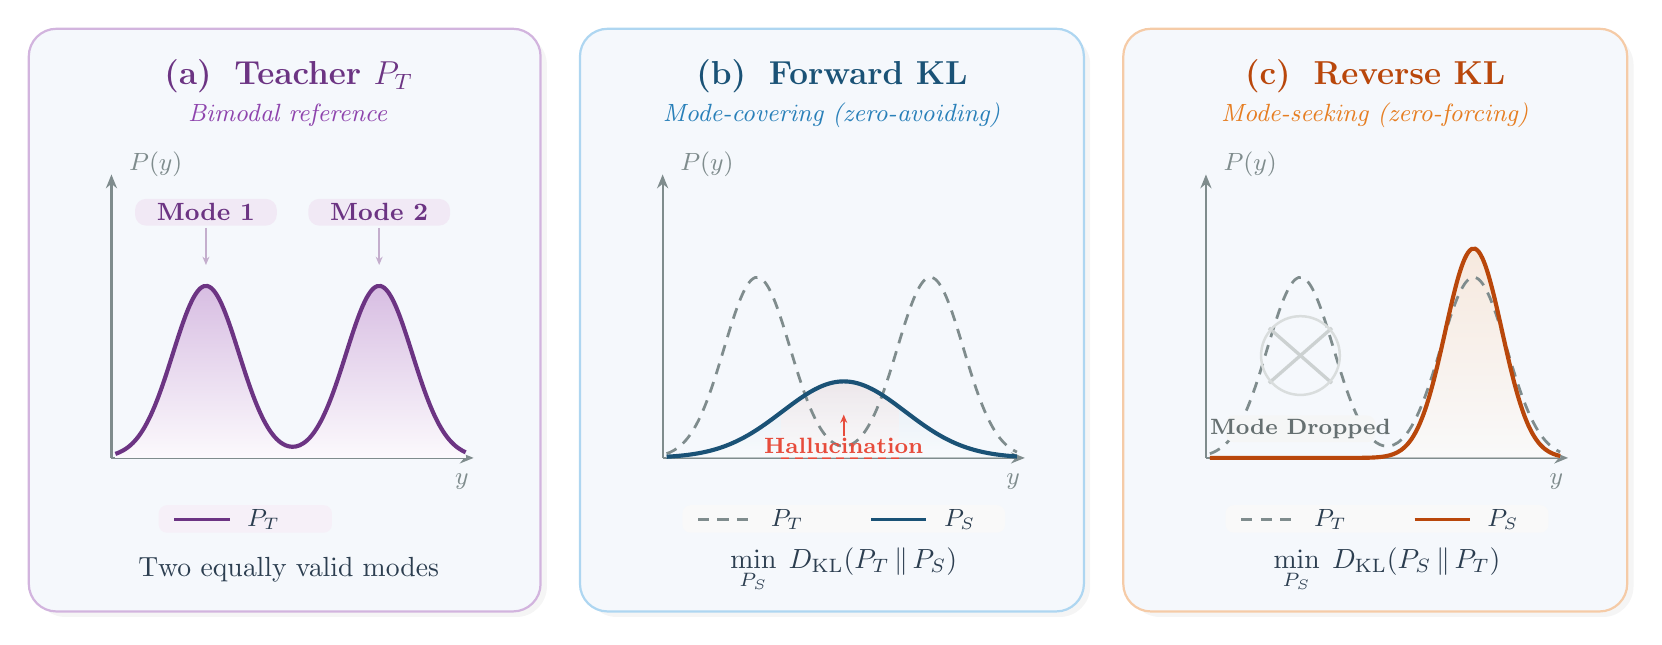
\begin{tikzpicture}[>=Stealth]

  % =================== Panel (a): Teacher P_T ===================
  \fill[black, opacity=0.04, rounded corners=11pt] (0.08, -1.87) rectangle (6.58, 5.53);
  \fill[panelbg, rounded corners=10pt] (0, -1.8) rectangle (6.5, 5.6);
  \draw[lightpurple, line width=0.8pt, rounded corners=10pt] (0, -1.8) rectangle (6.5, 5.6);

  \begin{scope}[shift={(1.05, 0.15)}]
    \node[font=\large\bfseries, deeppurple] at (2.25, 4.85) {(a)\; Teacher $P_T$};
    \node[font=\small, midpurple] at (2.25, 4.35) {\textit{Bimodal reference}};
    \draw[-{Stealth[length=5pt,width=4pt]}, line width=0.8pt, midgray]
      (0, 0) -- (4.6, 0);
    \node[font=\small, midgray, anchor=north] at (4.45, -0.08) {$y$};
    \draw[-{Stealth[length=5pt,width=4pt]}, line width=0.8pt, midgray]
      (0, 0) -- (0, 3.6);
    \node[font=\small, midgray, anchor=south west] at (0.1, 3.45) {$P(y)$};
    \shade[top color=midpurple!35, bottom color=midpurple!3, smooth, samples=100, domain=0.05:4.5]
      plot (\x, {2.3*(exp(-((\x-1.2)^2)/(2*0.42^2)) + exp(-((\x-3.4)^2)/(2*0.42^2)))/(0.42*sqrt(2*pi))})
      -- (4.5,0) -- (0.05,0) -- cycle;
    \draw[deeppurple, line width=1.5pt, smooth, samples=100, domain=0.05:4.5]
      plot (\x, {2.3*(exp(-((\x-1.2)^2)/(2*0.42^2)) + exp(-((\x-3.4)^2)/(2*0.42^2)))/(0.42*sqrt(2*pi))});
    \fill[midpurple!12, rounded corners=4pt] (0.3, 2.95) rectangle (2.1, 3.29);
    \node[font=\small\bfseries, deeppurple] at (1.2, 3.12) {Mode 1};
    \fill[midpurple!12, rounded corners=4pt] (2.5, 2.95) rectangle (4.3, 3.29);
    \node[font=\small\bfseries, deeppurple] at (3.4, 3.12) {Mode 2};
    \draw[-{Stealth[length=3pt,width=2.5pt]}, deeppurple!40, line width=0.6pt] (1.2, 2.92) -- (1.2, 2.45);
    \draw[-{Stealth[length=3pt,width=2.5pt]}, deeppurple!40, line width=0.6pt] (3.4, 2.92) -- (3.4, 2.45);
    \fill[midpurple!8, rounded corners=3pt] (0.6, -0.6) rectangle (2.8, -0.95);
    \draw[deeppurple, line width=0.9pt] (0.8, -0.78) -- (1.5, -0.78);
    \node[font=\small, deepgray, anchor=west] at (1.6, -0.78) {$P_T$};
    \node[font=\normalsize, deepgray] at (2.25, -1.42)
      {Two equally valid modes};
  \end{scope}

  % =================== Panel (b): Forward KL ===================
  \fill[black, opacity=0.04, rounded corners=11pt] (7.08, -1.87) rectangle (13.48, 5.53);
  \fill[panelbg, rounded corners=10pt] (7.0, -1.8) rectangle (13.4, 5.6);
  \draw[lightblue, line width=0.8pt, rounded corners=10pt] (7.0, -1.8) rectangle (13.4, 5.6);

  \begin{scope}[shift={(8.05, 0.15)}]
    \node[font=\large\bfseries, deepblue] at (2.15, 4.85) {(b)\; Forward KL};
    \node[font=\small, midblue] at (2.15, 4.35) {\textit{Mode-covering (zero-avoiding)}};
    \draw[-{Stealth[length=5pt,width=4pt]}, line width=0.8pt, midgray]
      (0, 0) -- (4.6, 0);
    \node[font=\small, midgray, anchor=north] at (4.45, -0.08) {$y$};
    \draw[-{Stealth[length=5pt,width=4pt]}, line width=0.8pt, midgray]
      (0, 0) -- (0, 3.6);
    \node[font=\small, midgray, anchor=south west] at (0.1, 3.45) {$P(y)$};
    \shade[top color=midblue!20, bottom color=midblue!2, opacity=0.5, smooth, samples=100, domain=0.05:4.5]
      plot (\x, {1.9*exp(-((\x-2.3)^2)/(2*0.78^2))/(0.78*sqrt(2*pi))})
      -- (4.5,0) -- (0.05,0) -- cycle;
    \draw[coralpink, line width=0.9pt, dash pattern=on 3pt off 2pt, smooth, samples=60, domain=1.5:3.0]
      plot (\x, {1.9*exp(-((\x-2.3)^2)/(2*0.78^2))/(0.78*sqrt(2*pi))});
    \draw[coralpink, line width=0.9pt, dash pattern=on 3pt off 2pt] (1.5, 0) -- (3.0, 0);
    \shade[top color=coralpink!18, bottom color=coralpink!2, opacity=0.4, smooth, samples=60, domain=1.5:3.0]
      plot (\x, {1.9*exp(-((\x-2.3)^2)/(2*0.78^2))/(0.78*sqrt(2*pi))})
      -- (3.0, 0) -- (1.5, 0) -- cycle;
    \draw[midgray, line width=1.0pt, dash pattern=on 4pt off 3pt, smooth, samples=100, domain=0.05:4.5]
      plot (\x, {2.3*(exp(-((\x-1.2)^2)/(2*0.42^2)) + exp(-((\x-3.4)^2)/(2*0.42^2)))/(0.40*sqrt(2*pi))});
    \draw[deepblue, line width=1.5pt, smooth, samples=100, domain=0.05:4.5]
      plot (\x, {1.9*exp(-((\x-2.3)^2)/(2*0.78^2))/(0.78*sqrt(2*pi))});
    \node[font=\footnotesize\bfseries, coralpink, inner sep=0pt] at (2.3, 0.15) {Hallucination};
    \draw[-{Stealth[length=3pt,width=2.5pt]}, coralpink, line width=0.7pt] (2.3, 0.28) -- (2.3, 0.55);
    \fill[midgray!5, rounded corners=3pt] (0.25, -0.6) rectangle (4.35, -0.95);
    \draw[midgray, line width=1.0pt, dash pattern=on 4pt off 3pt] (0.45, -0.78) -- (1.15, -0.78);
    \node[font=\small, deepgray, anchor=west] at (1.25, -0.78) {$P_T$};
    \draw[deepblue, line width=0.9pt] (2.65, -0.78) -- (3.35, -0.78);
    \node[font=\small, deepgray, anchor=west] at (3.45, -0.78) {$P_S$};
    \node[font=\normalsize, deepgray] at (2.3, -1.42)
      {$\displaystyle\min_{P_S}\; D_{\mathrm{KL}}(P_T \,\|\, P_S)$};
  \end{scope}

  % =================== Panel (c): Reverse KL ===================
  \fill[black, opacity=0.04, rounded corners=11pt] (13.98, -1.87) rectangle (20.38, 5.53);
  \fill[panelbg, rounded corners=10pt] (13.9, -1.8) rectangle (20.3, 5.6);
  \draw[lightorange, line width=0.8pt, rounded corners=10pt] (13.9, -1.8) rectangle (20.3, 5.6);

  \begin{scope}[shift={(14.95, 0.15)}]
    \node[font=\large\bfseries, deeporange] at (2.15, 4.85) {(c)\; Reverse KL};
    \node[font=\small, midorange] at (2.15, 4.35) {\textit{Mode-seeking (zero-forcing)}};
    \draw[-{Stealth[length=5pt,width=4pt]}, line width=0.8pt, midgray]
      (0, 0) -- (4.6, 0);
    \node[font=\small, midgray, anchor=north] at (4.45, -0.08) {$y$};
    \draw[-{Stealth[length=5pt,width=4pt]}, line width=0.8pt, midgray]
      (0, 0) -- (0, 3.6);
    \node[font=\small, midgray, anchor=south west] at (0.1, 3.45) {$P(y)$};
    \shade[top color=midorange!28, bottom color=midorange!3, opacity=0.5, smooth, samples=100, domain=0.05:4.5]
      plot (\x, {2.4*exp(-((\x-3.4)^2)/(2*0.36^2))/(0.36*sqrt(2*pi))})
      -- (4.5,0) -- (0.05,0) -- cycle;
    \draw[midgray, line width=1.0pt, dash pattern=on 4pt off 3pt, smooth, samples=100, domain=0.05:4.5]
      plot (\x, {2.3*(exp(-((\x-1.2)^2)/(2*0.42^2)) + exp(-((\x-3.4)^2)/(2*0.42^2)))/(0.40*sqrt(2*pi))});
    \draw[deeporange, line width=1.5pt, smooth, samples=100, domain=0.05:4.5]
      plot (\x, {2.4*exp(-((\x-3.4)^2)/(2*0.36^2))/(0.36*sqrt(2*pi))});
    \draw[midgray!40, line width=1.2pt] (0.8, 0.95) -- (1.6, 1.65);
    \draw[midgray!40, line width=1.2pt] (0.8, 1.65) -- (1.6, 0.95);
    \draw[midgray!30, line width=0.9pt] (1.2, 1.3) circle (0.5);
    \fill[midgray!8, rounded corners=3pt] (0.25, 0.2) rectangle (2.15, 0.54);
    \node[font=\footnotesize\bfseries, midgray!80!black] at (1.2, 0.37) {Mode Dropped};
    \fill[midgray!5, rounded corners=3pt] (0.25, -0.6) rectangle (4.35, -0.95);
    \draw[midgray, line width=1.0pt, dash pattern=on 4pt off 3pt] (0.45, -0.78) -- (1.15, -0.78);
    \node[font=\small, deepgray, anchor=west] at (1.25, -0.78) {$P_T$};
    \draw[deeporange, line width=0.9pt] (2.65, -0.78) -- (3.35, -0.78);
    \node[font=\small, deepgray, anchor=west] at (3.45, -0.78) {$P_S$};
    \node[font=\normalsize, deepgray] at (2.3, -1.42)
      {$\displaystyle\min_{P_S}\; D_{\mathrm{KL}}(P_S \,\|\, P_T)$};
  \end{scope}

\end{tikzpicture}
}
\caption{Forward KL vs.\ Reverse KL divergence for fitting a student distribution $P_S$ to a bimodal teacher $P_T$. \textbf{(a)}~The teacher places equal probability mass on two valid modes (e.g., two correct answers or two stylistic variants). \textbf{(b)}~Forward KL minimizes $\KL(P_T \parallel P_S)$ and is mode-covering (zero-avoiding): the student spreads a single broad Gaussian over both modes and places substantial probability in the inter-mode hallucination zone (red dashed boundary), corresponding to outputs that are a blend of the two valid answers and therefore neither. \textbf{(c)}~Reverse KL minimizes $\KL(P_S \parallel P_T)$ and is mode-seeking (zero-forcing): the student concentrates sharply onto a single peak (Mode 2), dropping Mode 1 entirely but producing crisp, coherent generations within the chosen mode. This trade-off motivates the adaptive-divergence methods in \S\ref{sec:objectives} (EOPD, AOPD), which interpolate between the two regimes based on per-token teacher entropy or log-ratio statistics.}
\label{fig:kl_divergence}
\end{figure*}

DistiLLM-2 applies different divergences to different data sources, but operates at a coarse granularity (entire sequences grouped by source). The fixed-divergence family faces a more fundamental limitation rooted in the heterogeneity of autoregressive token distributions \emph{within} a single sequence. The choice between Forward KL (mode-covering) and Reverse KL (mode-seeking) is a global decision applied uniformly across all token positions (Figure~\ref{fig:kl_divergence}). The teacher's distributional structure, however, varies considerably within a single sequence. At a mathematical operator token, the teacher concentrates probability mass on one or two correct symbols, so mode-seeking is appropriate because the student must commit to the correct answer. At a conjunction or filler word, dozens of tokens share comparable probability, so mode-covering is appropriate because any synonym suffices. Applying a single divergence to both positions therefore wastes gradient signal in one regime or discards coverage information in the other. This per-position mismatch between the geometry of the loss and the geometry of the target distribution motivates the adaptive methods of Section~\ref{subsec:adaptive_div}.

Sequence-level objectives offer a complementary perspective. MiniLLM~\citep{2306.08543} elevates Reverse KL to the full sequence level, where the student $\ptheta$ appears inside the sampling expectation. The central challenge is computing the gradient of an expectation over $\ptheta$ when $\ptheta$ itself is parameterized by $\theta$. Starting from $\KL(\ptheta \parallel \pteacher) = \E_{y \sim \ptheta}[\log \ptheta(y|x) - \log \pteacher(y|x)]$ and applying the policy gradient theorem, MiniLLM derives (Eq.~2 of~\citealp{2306.08543}):
\begin{equation}
    \nabla_\theta \loss_{\text{MiniLLM}} = -\E_{y \sim \ptheta} \left[ \sum_{t=1}^{|y|} (R_t - 1)\, \nabla_\theta \log \ptheta(y_t|y_{<t}) \right],\quad R_t = \sum_{t'=t}^{|y|} \log \frac{\pteacher(y_{t'}|y_{<t'})}{\ptheta(y_{t'}|y_{<t'})}
\end{equation}
where the $-1$ arises from the $-\log \ptheta(y|x)$ entropy term of the reverse-KL objective. Minimizing sequence-level Reverse KL is thus mathematically equivalent to policy gradient RL with per-step reward $r_t = \log[\pteacher(y_t|y_{<t}) / \ptheta(y_t|y_{<t})]$ and an entropy-induced constant. MiniLLM further decomposes $R_t$ into a single-step quality term and a future-return term (Eq.~3 of~\citealp{2306.08543}), computing $\E_{y_t \sim q_\theta}[r_t]$ in closed form over the vocabulary instead of by Monte Carlo sampling. This decomposition reduces variance by isolating the dominant source of gradient noise (single-step quality) from the accumulated future return, and supports credit assignment at the token level. Per-step returns $R_t$ attribute the trajectory's deviation from the teacher to specific token decisions rather than spreading uniform blame across the sequence, placing the optimization within the RL framework with the teacher's log-probability as a dense reward. This connection to policy optimization is consistent with MiniLLM's empirical strength on reasoning tasks where sequence-level coherence matters more than token-level accuracy, at the cost of higher training compute because REINFORCE estimation in combinatorial output spaces requires more iterations and careful baseline subtraction to converge. KETCHUP~\citep{2504.19024} addresses this variance problem by replacing the full cumulative return $G_t$ with a $K$-step Bellman return estimate derived from the optimality equation, reducing gradient variance at a power rate in $K$ while preserving the sequence-level objective (Theorem~1 of~\citealp{2504.19024}).

\textbf{The token-level vs.\ sequence-level tradeoff.} The choice between token-level and sequence-level objectives represents a core bias-variance tradeoff whose resolution foreshadows the RL-augmented methods of \S\ref{subsec:rl_objectives}. Token-level methods (GKD, DistiLLM) produce $|V|$-dimensional gradient signals at every position, resulting in low variance but potentially biased gradients when the teacher's token-level distribution is poorly calibrated (the flawed prefix trap of Section~\ref{subsec:weighting}). Sequence-level methods (MiniLLM, KETCHUP) yield unbiased gradients through the policy gradient theorem but suffer from high variance due to single-sample REINFORCE estimation over exponentially large sequence spaces. The practical resolution is task-dependent. For instruction following where token-level teacher quality is high, GKD-style methods tend to dominate. For reasoning tasks where sequence-level coherence matters more, MiniLLM-style methods are often preferred despite their variance, and KETCHUP's $K$-step Bellman returns offer an intermediate bias-variance point on this spectrum. Recognizing that MiniLLM is already performing policy gradient RL (with the teacher's log-probability as reward) suggests that sequence-level distillation and RL-augmented distillation are not distinct paradigms but endpoints of a continuum parameterized by the reward source, with pure teacher signal at one end, pure task reward at the other, and hybrid objectives (G-OPD, RLKD) interpolating between them.

\textbf{Full-vocabulary vs.\ sampled-token KL.} Orthogonal to the token-level vs.\ sequence-level choice, a practical implementation decision determines how much of the teacher's distribution is used at each position. Many RL-based OPD implementations approximate the per-position KL by computing $\log \ptheta(y_t|y_{<t}) - \log \pteacher(y_t|y_{<t})$ only at the \emph{sampled} token $y_t$, treating this scalar as a per-token advantage within a policy gradient framework~\citep{lu2025onpolicy}. While computationally lightweight (requiring only one teacher log-probability per position), this single-sample estimate incurs high gradient variance and discards the distributional information across non-sampled tokens. DeepSeek-V4~\citep{deepseekv4} reports that \emph{full-vocabulary} logit distillation, computing the exact $\KL(\ptheta(\cdot|y_{<t}) \parallel \pteacher(\cdot|y_{<t}))$ over all $|V|$ tokens at each position, yields more stable gradients and more faithful knowledge transfer at the cost of transmitting or reconstructing the full teacher logit vector. Their engineering solution (caching teacher hidden states and reconstructing logits on-the-fly through the prediction head) makes this feasible even with 10+ trillion-parameter teachers over vocabularies exceeding 100K tokens, which positions full-vocabulary KL as an attractive choice for industrial-scale OPD when infrastructure permits. Lightning-OPD~\citep{2604.13010} further reports that the full teacher forward pass can be largely avoided by precomputing teacher log-probabilities over SFT rollouts, recording 4.0$\times$ speedup over standard OPD under a \emph{teacher consistency} condition (using the same teacher for both SFT data generation and distillation).

\textbf{Divergence ascent for deliberation.} AntiSD~\citep{2605.11609} reverses the self-distillation gradient entirely. A pointwise mutual information analysis shows that privileged-context conditioning inflates the teacher's confidence on tokens already implied by the solution (structural connectives, verifiable claims) while deflating it on deliberation tokens (\textit{Wait}, \textit{Let}, \textit{Maybe}) that drive multi-step search. By \emph{ascending} the student-teacher divergence instead of descending it, AntiSD flips the per-token sign, yielding a naturally bounded advantage that boosts deliberation tokens in a single update step. An entropy-triggered gate disables the anti-distillation term once teacher entropy collapses, preventing degenerate behavior when the teacher distribution is already peaked. Across five models from 4B to 30B parameters, AntiSD matches GRPO accuracy in 2--10$\times$ fewer training steps and improves final accuracy by up to 11.5 points on math reasoning, suggesting that the standard ``descend toward the teacher'' assumption can be relaxed when the privileged signal is systematically biased.

\textbf{Control variate variance reduction.} vOPD~\citep{2605.07865} offers a third resolution to this variance-cost tradeoff by importing the \emph{control variate baseline} from policy-gradient RL into the OPD estimator. Casting the single-sample OPD gradient (Eq.~3 of~\citealp{2605.07865}) as a REINFORCE update with per-token reward $r_t = \log \pteacher(y_t|c_t) - \log \ptheta(y_t|c_t)$, vOPD subtracts a baseline $b_t(c_t)$ from $r_t$ before multiplying by $\nabla_\theta \log \ptheta$. The natural value function for this reward admits a closed form as the per-token negative reverse KL between student and teacher, $V^{\pi_\theta}(c_t) = -\KL(\ptheta(\cdot|c_t) \parallel \pteacher(\cdot|c_t))$, computable directly from the forward pass that already produces the OPD objective without requiring an auxiliary critic or additional rollouts. Because the baseline depends only on the context $c_t$ and not on the sampled token $y_t$, subtracting it preserves the unbiasedness of the gradient while reducing variance. A top-$k$ approximation of this baseline (restricting the KL summation to the student's $k$ most probable tokens) further lowers compute, and because the approximation remains independent of the sampled action, unbiasedness still holds regardless of $k$. Across six reasoning benchmarks on Qwen3-1.7B and 4B, vOPD yields an average +3\% absolute gain over vanilla single-sample OPD (up to +6.2\% on MATH500), matches the accuracy of full-vocabulary OPD while reducing wall-clock time by up to 57.7\%, and broadly outperforms top-$k$ OPD, which adds compute but introduces bias. The result positions vOPD at a favorable point on the bias-variance-compute Pareto frontier for on-policy distillation of reasoning models.

\textbf{Advantage and gradient redesigns within fixed-divergence training.} The variance-control results above retain the conventional advantage and gradient definitions and tune only the estimator. A complementary line of work asks whether the advantage itself is correctly specified once the on-policy rollout enters the picture. OPD+~\citep{2606.01039} re-derives the per-token weight from an $f$-divergence gradient analysis and observes that the conventional stop-gradient reward $r_t = \log[\pteacher(y_t|y_{<t})/\ptheta(y_t|y_{<t})]$ corresponds to $f(u) = -\log u$ but ignores the second-order curvature, and the gradient-faithful weight $w_f(u) = -f(u) + u\,f'(u)$ aligns the OPD update with the true $f$-divergence gradient and reduces a systematic bias that grows when the student strays far from the teacher. Where OPD+ corrects the per-token advantage, Bridging Reasoning Trajectories~\citep{2606.00305} addresses the short-horizon trajectory signal by detecting trajectory-level divergence through a short-window optimal-transport distance and injecting an OT-based teacher signal whenever the student's near-future continuation drifts away from teacher trajectories. Low-OT but high-loss tokens are downweighted to suppress false alarms, and a two-stage schedule (off-policy warmup followed by on-policy distillation) confines the OT correction to the on-policy regime where it is most informative. The same per-position-mismatch concern reappears for vision-language students, where reverse-KL gradients can be dominated by the language prior and effectively bypass visual grounding. Decomposed-OPD~\citep{2606.00564} responds with Visual Gradient Steering (VGS), a decomposition that splits the per-token gradient into a language-prior component and a visual-grounding component, normalizes the two by gradient norm, and amplifies the visual component by a Visual Dependency Score (VDS) read off from cross-attention statistics. A language-preservation regularizer prevents the rebalanced gradient from degrading text-only competence. Together, these three methods illustrate that the same fixed-divergence skeleton can be improved by acting on three distinct levels of the gradient signal, namely the per-token weight (OPD+), the short-horizon trajectory (Bridging), and the modality decomposition (Decomposed-OPD), without changing the divergence type itself.

\textbf{Proximal and DAgger-style reformulations.} Two further methods retain the fixed-divergence template but redefine \emph{what is being constrained}. Surgical Post-Training~\citep{2603.01683} treats reasoning injection as proximal on-policy distillation under a KL constraint to the pre-update policy, with the analytical and empirical claim that this KL-constrained reward formulation is what supports retention of existing capabilities during reasoning specialization. Distributional DAgger~\citep{2606.05152} returns to the original DAgger~\citep{1011.0686} blueprint that motivated GKD and generalizes scalar feedback into a teacher distribution. The student rolls out under its own policy, the feedback (e.g., a verifier or rich preference signal) conditions an EMA self-teacher, and the resulting forward cross-entropy is paired with a REINFORCE future-credit term so that token-level updates account for downstream consequences inside a PPO-style trust region. A top-$K$ teacher truncation keeps the per-token cost bounded. These two reformulations frame fixed-divergence OPD as an instance of constrained policy improvement, with KL-constrained reward acting as the retention mechanism (Surgical Post-Training) and a future-aware DAgger update acting as the credit-assignment mechanism (Distributional DAgger), both of which set up the per-position adaptive divergences of Section~\ref{subsec:adaptive_div}.

\subsection{Adaptive Divergence Objectives}
\label{subsec:adaptive_div}

\begin{table*}[t]
    \centering
    \caption{OPD methods: Adaptive divergence objectives.}
    \label{tab:methods_adaptive_div}
    \resizebox{\textwidth}{!}{
    \begin{tabular}{@{}lclllll@{}}
        \toprule
        \textbf{Method} & \textbf{Year} & \textbf{Category} & \textbf{Divergence/Objective} & \textbf{Signal} & \textbf{Granularity} & \textbf{Key Innovation} \\
        \midrule
        EOPD \citep{2603.07079} & 2026 & Objective & Continuous FKL+RKL blend & White-box & Token & Entropy-aware on-policy distillation \\
        AOPD \citep{2605.06387} & 2026 & Objective & Asymmetric PG/FKL switch & White-box & Token & Advantage-sign token-level switching \\
        CREDIT \citep{2605.11613} & 2026 & Self (EF) & Contrastive pMI decomposition & Self (contrastive) & Token & Input-specific credit for OPSD reward \\
        OGLS-SD \citep{2605.12400} & 2026 & Self (EF) & Outcome-guided logit steering & Self (outcome) & Token & Outcome-based teacher calibration \\
        Position-Weighted OPSD \citep{2605.21606} & 2026 & Objective & Position-aware reliability & Self (PI) & Token & Per-position reliability score \\
        Direction-Adaptive SD \citep{2605.22263} & 2026 & Objective & Entropy-routed polarity & Self (PI) & Token & High-entropy teacher reversal \\
        Token-Teachability \citep{2605.26844} & 2026 & Objective & Teachability-gated KL & White-box & Token & Fixed-context learnability diagnostic \\
        Lookahead Group Reward \citep{2605.30833} & 2026 & Objective & RKL + look-ahead group reward & White-box & Token & One-step-ahead teacher confidence \\
        RAFT \citep{2606.00147} & 2026 & Objective & Top-$K$ temperature distill & Self & Token & Data refinement + EMA loss balance \\
        Trust-Region OPD \citep{2606.01249} & 2026 & Objective & Adaptive trust-region KL & White-box & Token & Speculative-decoding-ratio gating \\
        GNDPO \citep{2606.09091} & 2026 & Objective & Global batch-normalized KL & White-box & Token & Batch-relative KL normalization for MLLM stability \\
        \bottomrule
    \end{tabular}
    }
\end{table*}

Adaptive methods tackle this per-position mismatch by selecting or interpolating divergences based on local distributional geometry (Table~\ref{tab:methods_adaptive_div}). When the teacher is certain (low entropy), mode-seeking Reverse KL preserves precision, and when uncertain (high entropy), mode-covering Forward KL preserves diversity.

EOPD~\citep{2603.07079} uses the teacher's per-token entropy $H(\pteacher(\cdot|y_{<t}))$ as a gating signal. The base objective is Reverse KL at all positions, with Forward KL \emph{additively} activated at high-entropy tokens where the teacher distributes probability across multiple valid continuations:
\begin{equation}
    \loss_{\text{EA}} = \E_{y \sim \ptheta} \left[ \sum_{t=1}^{|y|} \KL(\ptheta \parallel \pteacher) + \mathbb{I}[H_t > \tau_H] \cdot \KL(\pteacher \parallel \ptheta) \right]
\end{equation}
EOPD outperforms fixed divergence baselines on math reasoning (MATH, GSM8K) and open-ended generation (AlpacaEval), consistent with the view that the appropriate divergence is position-dependent. Conditioning on teacher uncertainty alone (a marginal property) gives EOPD a stable routing signal independent of student quality, making it suitable for early training when the student's distribution is less reliable.

\textbf{Self-distillation reward calibration.} Two recent methods address pathologies specific to the self-distillation reward signal by injecting contrastive or outcome-based corrections. CREDIT~\citep{2605.11613} decomposes the standard OPSD token reward into input-specific and input-generic components via a batch-contrastive baseline, suppressing generic shortcuts that inflate pointwise mutual information without contributing task-relevant reasoning (Section~\ref{subsec:external_feedback}). OGLS-SD~\citep{2605.12400} calibrates the self-reflected teacher distribution using verifiable outcome rewards to contrast successful and failed on-policy trajectories, addressing reflection-induced bias that shifts teacher logits away from optimal targets (Section~\ref{subsec:external_feedback}). Both methods operate within the self-distillation paradigm and are detailed in Section~\ref{subsec:external_feedback}.

AOPD~\citep{2605.06387} extends the per-token adaptive principle by diagnosing \emph{why} standard OPD gradients fail at specific token positions. In non-positive advantage regions ($A_t \le 0$), standard advantage-weighted policy gradients exhibit three pathologies that intensify under weak initialization. Heavy-tailed variance from unbounded negative advantages destabilizes updates, vanishing gradients at zero-advantage positions waste teacher signal, and ``exploration black holes'' trap learning because suppressing a wrong token only redistributes mass proportional to the student's own prior, unable to boost low-probability correct alternatives. AOPD addresses this by switching the objective at the token level. For positive-advantage tokens ($A_t > 0$), standard policy gradient exploitation is preserved. For non-positive tokens, the framework substitutes localized forward-KL guidance on the teacher's top-$K$ support, creating an asymmetric exploitation-imitation mechanism. A threshold parameter $\tau$ (set to zero by default, corresponding to the probability difference between teacher and student) determines the switching point, with $\tau = -1$ recovering standard OPD (intervention rarely triggers because $P_T - P_S \le -1$ is almost never satisfied) and $\tau = 1$ recovering GKD (intervention everywhere because $P_T - P_S \le 1$ generally holds). On competition-level mathematics (AIME 2024/2025, HMMT), AOPD attains average gains of +4.09 with strong initialization and +8.34 with weak initialization over standard on-policy baselines, with the weak-initialization gap suggesting that the exploration black hole is among the dominant failure modes when the student starts far from the teacher. AOPD adapts the \emph{objective class itself} (policy gradient vs.\ divergence minimization) based on the gradient's structural health at each position, complementing entropy-based routing in EOPD that adapts the divergence \emph{type}.

\textbf{Token reliability and teachability.} A complementary line of work refines per-token routing by replacing implicit signals (teacher entropy, advantage sign) with direct measurements of how trustworthy or learnable each position is. Position-Weighted OPSD~\citep{2605.21606} observes that teacher entropy alone is insufficient to predict supervision quality at a given position, and that reliability degrades with depth into the student rollout because later positions condition on increasingly off-policy prefixes. The method modulates the per-token loss by a position-aware reliability score read off from teacher behavior on student-generated sequences, recovering accuracy where uniform weighting flattens the gradient. Token-Teachability OPD~\citep{2605.26844} attacks the same problem from the student side. A fixed-context diagnostic measures whether the student can plausibly absorb the teacher's preferred token at each position, separating genuinely learnable tokens from tokens that are merely high-disagreement. Selective OPD restricted to teachable tokens outperforms entropy-based and disagreement-based selection on reasoning benchmarks. Together, the two methods localize where the teacher's signal carries useful information (Position-Weighted) and where the student is in a position to use it (Token-Teachability), tightening the routing logic that EOPD and AOPD apply at coarser per-position granularities. Direction-Adaptive Self-Distillation~\citep{2605.22263} pushes the routing further by reversing the teacher's polarity at high-entropy tokens, similar in spirit to AntiSD's divergence ascent (Section~\ref{subsec:fixed_div}) but gated on entropy as in EOPD, so that the student is pulled away from the teacher at deliberation points where teacher uncertainty signals exploration value rather than guidance value.

\textbf{Look-ahead and trust-region adaptation.} Per-position routing can also be improved by extending the teacher signal across positions or by gating updates by stability. Lookahead Group Reward~\citep{2605.30833} identifies \emph{Supervision Fidelity Decay}, the observation that per-token teacher confidence on student rollouts degrades along the trajectory as the student drifts off-policy. The method augments the per-token signal with a one-step-ahead group reward, computing teacher confidence under a tree-attention mask after a single look-ahead step, group-normalizing the resulting score, and gating its activation on local entropy. Trust-Region OPD~\citep{2606.01249} adapts the per-step trust region directly. The acceptance ratio of speculative decoding is repurposed as a cheap proxy for student-teacher policy divergence, an outlier estimator clips top-$k$ FKL excursions, and an off-policy teacher prefix is mixed in with cosine annealing during early training when the student rollout is least informative. The K1 reverse-KL estimator anchors the resulting trust region, recovering the EOPD and AOPD gating principle at the trajectory level. RAFT~\citep{2606.00147} couples the same adaptive principle to the data side by alternating self-conditioned rewriting (which refines noisy domain prompts via cosine-similarity semantic filtering and multi-expert fusion) with answer-conditioned on-policy distillation that uses top-$K$ temperature distillation against the original instruction-tuned model. An EMA-based adaptive loss balancer keeps the distillation and SFT components from interfering, supporting the broader observation that on-policy distillation in domain specialization regimes benefits from adapting both the data distribution and the per-token weight.

\textbf{Batch normalization for stable on-policy distillation.} GNDPO~\citep{2606.09091} addresses an instability that arises when adaptive KL losses are applied to multimodal LLMs (MLLMs). Standard per-sample KL normalization can produce large gradient variance across mini-batches when the token-count distribution varies widely (e.g., vision inputs of different resolutions). GNDPO normalizes the KL objective across the entire batch relative to a global reference distribution, producing smoother gradient estimates and more stable training dynamics for MLLMs trained with on-policy distillation.

The field has moved noticeably from ``which divergence?'' to ``which divergence \emph{where}?'' The evidence from EOPD and AOPD points to a consistent finding across evaluated settings, namely that no single fixed divergence dominates uniformly, and that even the simplest adaptive routing (a hard entropy threshold) often outperforms the best-tuned fixed alternative. Yet adaptive divergences, however sophisticated their per-token routing, share a structural limitation with their fixed counterparts. They optimize a distance to the teacher distribution. Perfect optimization under any $f$-divergence yields a student that matches the teacher but rarely exceeds it. When the teacher itself makes errors or lacks reasoning paths that a well-guided student could discover, divergence minimization can act more as a ceiling than as a floor.

\subsection{RL-Augmented Objectives}
\label{subsec:rl_objectives}

\begin{table*}[t]
    \centering
    \caption{OPD methods: RL-augmented objectives.}
    \label{tab:methods_rl}
    \resizebox{\textwidth}{!}{
    \begin{tabular}{@{}lclllll@{}}
        \toprule
        \textbf{Method} & \textbf{Year} & \textbf{Category} & \textbf{Divergence/Objective} & \textbf{Signal} & \textbf{Granularity} & \textbf{Key Innovation} \\
        \midrule
        G-OPD \citep{2602.12125} & 2026 & Objective & KL-Constrained RL & White-box & Token/Seq & OPD $\equiv$ dense KL-RL, reward extrapolation \\
        RLKD \citep{2505.16142} & 2025 & Objective & KD + Reward Model & Reward Model & Sequence & Generative Structure Reward Model (GSRM) \\
        KDRL \citep{2506.02208} & 2025 & Objective & Joint KD + RL & White-box & Token/Seq & On-policy KL regularizer during RL \\
        RLAD \citep{2602.22495} & 2026 & Objective & Trust Region Ratio & White-box & Token/Seq & PPO-style selective teacher following \\
        AlignDistil \citep{2503.02832} & 2025 & Objective & DPO + Reverse DPO & White-box & Token & Token-level RLHF via contrastive DPO reward \\
        SuperCorrect \citep{2410.09008} & 2024 & Objective & Template + Cross-DPO & White-box & Sequence & Hierarchical thought scaffolding \\
        SCoRe \citep{2509.14257} & 2025 & Objective & Earliest-error correction & White-box & Sequence & Root-cause error targeting \\
        CMDP-KD \citep{2509.22921} & 2025 & Objective & Constrained KL & White-box & Sequence & Unaugmented CMDP with hard KL budget \\
        $\mathcal{X}$-KD \citep{2602.12674} & 2026 & Objective & Inverse RL + KL & White-box & Token/Seq & AVRIL-based reward recovery distillation \\
        TSD-KD \citep{2603.13260} & 2026 & Objective & Indirect + Direct KD & White-box & Sequence & Indirect re-ranking + selective direct KL \\
        REOPOLD \citep{2603.11137} & 2026 & Objective & Log-ratio token reward & White-box & Token & Mixture reward clipping + entropy-dynamic sampling \\
        CoDistill-GRPO \citep{2605.08873} & 2026 & Objective & GRPO + KD reward & White-box & Sequence & Bidirectional co-distillation, 18\% speedup \\
        dGRPO \citep{2605.12227} & 2026 & Objective & GRPO + dense OPD & White-box & Token/Seq & Long-context reasoning with LongBlocks data \\
        Sparse-to-Dense \citep{2605.12483} & 2026 & Objective & Staged RL$\to$OPD$\to$RL & White-box & Token/Seq & Reward-density allocation principle \\
        TGPO \citep{2605.13230} & 2026 & Objective & Directional teacher PG & White-box & Token & Dense directional teacher guidance on RKL \\
        RWOPD \citep{2605.13501} & 2026 & Objective & Verifier-weighted FKL & White-box & Sequence & Verifier-reward-weighted OPD for NL2SVA \\
        AMR-SD \citep{2605.18529} & 2026 & Objective & Asymmetric meta-reflective & Self & Token & Meta-reflection self-teacher in RLVR \\
        OPPO \citep{2605.21851} & 2026 & Objective & Bayesian value recursion & Oracle (PI) & Token & Likelihood-ratio per-token credit \\
        StepOPSD \citep{2605.27140} & 2026 & Objective & Step-aware preference + KL & Self (hindsight) & Step/Token & Dual-granularity for multi-turn agents \\
        Self-Eval OPD \citep{2606.05122} & 2026 & Objective & Cyclic GRPO + masked judge KD & External judge & Token & Self-evaluation channel calibration \\
        RLCSD \citep{2606.11709} & 2026 & Objective & Contrastive RKL in GRPO & White-box & Token & Correct-hint teacher pull, wrong-hint push in two-path distillation \\
        \bottomrule
    \end{tabular}
    }
\end{table*}

Divergence matching, whether fixed or adaptive, tends to bound the student near the teacher's capability ceiling (Table~\ref{tab:methods_rl}). In the limit of perfect optimization, the student matches the teacher's distribution and rarely exceeds it. RL-augmented objectives target this limitation by injecting an external performance signal that can steer the student toward solutions the teacher itself would be unlikely to produce.

\textbf{OPD as KL-constrained RL.} G-OPD~\citep{2602.12125} formalizes an equivalence between standard OPD and dense KL-constrained reinforcement learning. It formulates distillation as maximizing a token-level reward defined as the log-probability ratio between teacher and reference policy, penalized by KL divergence from the reference:
\begin{equation}
    \max_\theta \E_{y \sim \ptheta} \left[ \sum_{t=1}^{|y|} \alpha \log \frac{\pteacher(y_t | y_{<t})}{p_{\text{ref}}(y_t | y_{<t})} - \KL\big(\ptheta(\cdot | y_{<t}) \parallel p_{\text{ref}}(\cdot | y_{<t})\big) \right]
\end{equation}
When $\alpha = 1$, this reduces to standard Reverse KL distillation. When $\alpha > 1$, the objective forces the student to \emph{extrapolate} beyond the teacher's probability mass, allowing a phenomenon documented as \emph{Reward Extrapolation}, whereby the student discovers previously unseen, structurally sound reasoning paths in regions where the teacher's generation probability $\pteacher(y|x)$ is low but the outcome reward remains high. In the multi-teacher setting where several domain-specific RL experts share the same base model, reward extrapolation (ExOPD) produces a unified student that surpasses all its same-size domain teachers, suggesting that OPD need not be a lossy compression step.

This equivalence carries a broader consequence for the section as a whole. It connects the distillation and RL communities by indicating that the objectives discussed here (GKD's token-level KL, MiniLLM's sequence-level Reverse KL, G-OPD's reward-augmented formulation) can be viewed as special cases of KL-constrained policy optimization with different reward definitions and constraint strengths. Advances in KL-constrained RL (better trust regions, adaptive penalty coefficients, variance reduction) are therefore likely to transfer to OPD, and vice versa.

\textbf{Gradient decomposition and the KD+RL complementarity.} The unified KD+RL framework of~\citet{2512.23097} decomposes the hybrid gradient into two complementary components, a dense KD gradient for token-level imitation and a Monte Carlo RL gradient for reward maximization. The KD component dampens the high variance inherent in policy gradient estimation, while the RL component prevents the student from collapsing onto teacher modes that are suboptimal for the downstream task. REOPOLD~\citep{2603.11137} instantiates this insight by interpreting on-policy distillation as policy optimization where the teacher-student log-likelihood ratio acts as a token reward. It stabilizes training through three mechanisms, namely mixture-based reward clipping to prevent over-trust of extreme teacher signals, entropy-based dynamic sampling that selectively weights teacher feedback at high-uncertainty tokens, and a unified exploration-to-refinement schedule. Empirically, REOPOLD attains 6.7--12$\times$ greater sample efficiency than recent RL approaches and allows a 7B student to match a 32B teacher in visual reasoning with $\sim$3.3$\times$ inference speedup.

\textbf{Structure-aware reward as an alternative to dense KL.} While G-OPD and REOPOLD retain token-level KL as the primary distillation signal (differing only in how they augment or stabilize it), RLKD~\citep{2505.16142} departs from this template entirely by replacing token-level KL with a Generative Structure Reward Model (GSRM). The GSRM parses both teacher and student reasoning paths into sequences of meta-reasoning and solving steps, then scores structural alignment between the two sequences. This structural reward is combined with a task-level outcome reward (e.g., math accuracy) and optimized via GRPO:
\begin{equation}
    R_{\text{total}}(x, y) = \alpha \, R_{\text{GSRM}}(y, y^{\text{teach}}) + (1-\alpha) \, R_{\text{outcome}}(x, y)
\end{equation}
The main idea is that reasoning distillation need not operate at the token level. By supervising at the \emph{step structure} level, RLKD avoids the vocabulary-coupling assumption of logit-based methods while still transferring the teacher's multi-branch reasoning strategy. Empirically, RLKD trained on only 0.1\% of the data under a pure RL regime surpasses standard SFT-RL pipelines, showing that structural reward can substitute for dense KL when the teacher's value lies in its reasoning organization rather than its token-level distribution. This progression from dense token-level KL (G-OPD) through variance-reduced token rewards (REOPOLD) to step-level structural matching (RLKD) traces an increasing abstraction of what ``teacher knowledge'' means, moving from distributional fidelity to behavioral organization.

\textbf{Bidirectional co-distillation.} CoDistill-GRPO~\citep{2605.08873} addresses the common failure of GRPO on small models (where sparse rewards on difficult tasks yield negligible learning signal) through a co-distillation algorithm that simultaneously trains a large and a small model with carefully designed GRPO objectives. The small model uses an on-policy KD reward derived from the large model's distribution as dense supervision, while the large model trains on the small model's rollouts with importance reweighting, reducing the computational overhead of rollout generation. On Qwen2.5-Math-1.5B, CoDistill-GRPO yields an accuracy increase of over 11.6 percentage points over the base model and 6.0 points over standard GRPO on Minerva. The large model (Qwen2.5-Math-7B) nearly matches standard GRPO despite training on small-model rollouts, providing an approximate 18\% speedup. The bidirectional design avoids the common assumption that a pre-trained oracle must exist, instead producing both the teacher signal and the student improvement simultaneously.

\textbf{Directional teacher guidance on reverse KL.} TGPO~\citep{2605.13230} departs from the additive KD+RL template by embedding teacher guidance \emph{inside} the policy gradient itself. Rather than treating the teacher's distribution as a separate regularization term, TGPO uses the teacher's per-token likelihood ratio as a directional signal that steers the reverse-KL gradient toward regions the teacher considers promising, concentrating updates on tokens where teacher and student disagree most. This dense directional coupling avoids the balancing hyperparameter that joint KD+RL objectives require (the $\alpha$ in RLKD, the KL penalty in KDRL) and instead lets the teacher's confidence modulate the RL gradient at every position. On math reasoning benchmarks (e.g., MATH-500), TGPO outperforms both standalone OPD and standalone GRPO, consistent with the view that tighter coupling between teacher guidance and policy optimization can be more effective than additive combination.

\textbf{Dense guidance for long-context reasoning.} dGRPO~\citep{2605.12227} targets the same sparse-reward failure mode as CoDistill-GRPO but through a different architecture. Rather than co-training two models, dGRPO augments a single student's GRPO training with dense token-level guidance from a stronger teacher via an additive OPD term. The method specifically targets the long-context reasoning regime (8K--32K tokens), where sparse rewards are especially unstable because correct reasoning paths become increasingly rare in longer sequences and the effective learning signal degrades with context length. The accompanying LongBlocks dataset provides synthetic long-context tasks spanning multi-hop reasoning, contextual grounding, and long-form generation. The combined KD+RL objective provides more stable optimization than either component alone, addressing the regime where pure GRPO suffers from sample inefficiency (most long-context rollouts fail entirely) and pure OPD lacks direct reward optimization for discovering previously unseen long-range reasoning patterns. Where CoDistill-GRPO uses the KD signal bidirectionally between two models, dGRPO applies it unidirectionally from a fixed teacher, trading the mutual bootstrapping benefit for architectural simplicity.

\textbf{Sparse-to-dense reward allocation.} \citet{2605.12483} articulate a reward-density principle that reframes GRPO and OPD not as competing recipes but as different reward-density regimes. Sparse sequence-level reward is most productive on the strongest model where exploration can discover new solutions (teacher-side RL), while dense token-level teacher reward is most effective for compressing learned behavior into a smaller model (student-side OPD). The operational lesson is a three-stage pipeline, namely GRPO on the teacher for capability discovery, a forward-KL warmup followed by OPD as a dense bridge, and optional student-side sparse RL after the bridge. At fixed Qwen3-1.7B deployment size, an RL-improved 8B teacher distilled through this dense bridge outperforms direct GRPO on the student (79.3\% vs.\ 75.9\% on MATH, 25.2 vs.\ 19.8 on AIME 2024), while transfer from the same teacher \emph{before} RL underperforms. The bridge also makes subsequent student-side GRPO effective where it previously was not, lifting MATH from 75.4\% to 78.5\%. The teacher-quality ordering replicates on Llama-3.1-8B-Instruct with a Llama-3.3-70B-Instruct teacher.

\textbf{Joint vs.\ sequential optimization.} Given that KD and RL supply complementary gradient signals (dense imitation vs.\ sparse reward maximization), a persistent engineering challenge is \emph{how} to combine them within a single training pipeline without mutual interference. Sequential approaches (distill-then-RL or RL-then-distill) tend to suffer from catastrophic interference, as the RL stage degrades distilled knowledge through policy drift, while the KD stage suppresses previously unseen solutions discovered through exploration. KDRL~\citep{2506.02208} implements joint optimization by adding an on-policy KL regularizer between student and teacher \emph{during} RL training, mitigating policy drift while still allowing reward-driven exploration. CMDP-KD~\citep{2509.22921} extends this regularization scheme by replacing the soft KL penalty with a \emph{hard} KL budget via constrained MDP formulation. The state-augmented Saute formulation can be simplified for LLMs by removing state augmentation entirely, since the full history already determines the remaining budget, yielding constraint satisfaction guarantees without requiring teacher access at inference. RLAD~\citep{2602.22495} refines this further by recognizing that unconditional KL regularization is itself suboptimal. Its Trust Region Ratio Distillation (TRRD) replaces the standard KL penalty with a PPO-style likelihood-ratio objective anchored to a teacher-old-policy mixture. This selective strategy follows the teacher only when its signal improves the policy update, preventing blind KL minimization from dragging the student toward suboptimal trajectories on problems the teacher itself cannot solve. The progression from KDRL's uniform regularization to RLAD's selective trust region mirrors the fixed-to-adaptive evolution in divergence objectives (Section~\ref{subsec:fixed_div}$\to$\ref{subsec:adaptive_div}), echoing a recurring pattern across this survey that conditioning the learning signal on local geometry often works better than applying it uniformly.

\textbf{Preference-based objectives as implicit RL.} When logit access is unavailable or when sequence-level quality judgments are more natural than token-level distributions, several methods map the KD+RL problem onto Direct Preference Optimization (DPO). AlignDistil~\citep{2503.02832} derives token-level rewards from contrastive DPO and reverse DPO models, converting sequence-level RLHF into per-token policy distillation that applies both standard and reverse preference objectives at the token granularity. OVD~\citep{2601.21968} queries the teacher for pairwise preferences over student-generated responses, avoiding continuous probability extraction entirely. These preference-based objectives share a deep connection to token-level KL methods. Under DPO's closed-form solution, the optimal policy satisfies $\pi^*(y|x) \propto \pi_{\text{ref}}(y|x) \exp(r(y,x)/\beta)$, and substituting the teacher's log-probability as the implicit reward yields the geometric mixture distribution targeted by GKD with $\lambda$-mixing. The practical implication is that DPO-style methods are often most useful when constructing preference pairs is cheaper than computing full teacher logits. PBSD~\citep{2605.05040} pushes this connection further in the self-distillation regime by deriving the reward-regularized optimum $\pi^* \propto \pi_{\text{teach}} \exp(r/\beta)$ against a context-augmented teacher rather than a static reference policy, and suggesting that this reward-tilted target improves over the teacher itself under the same objective whenever the reward is non-degenerate (Section~\ref{subsec:self_pi}). The spectrum exposes a unifying gradient. Token-level KL (G-OPD, REOPOLD), step-level structure matching (RLKD), and sequence-level preference ranking (AlignDistil, OVD) all implement KL-constrained policy optimization at different abstraction levels, with the appropriate level determined by signal availability and the granularity at which teacher expertise manifests.

\textbf{Verifier-reward-weighted distillation.} When a domain-specific verifier can assign correctness scores to student rollouts, these scores offer a natural per-sample weighting for the distillation objective. RWOPD~\citep{2605.13501} instantiates this idea for NL-to-SystemVerilog generation, where an open property-equivalence verifier scores each student-generated hardware description against a formal specification. The verifier reward weights the forward-KL loss so that rollouts closer to functional correctness receive stronger teacher supervision, while clearly incorrect rollouts are attenuated rather than discarded entirely (preserving gradient signal from partial successes). The approach sets new benchmarks on NL2SVA benchmarks, suggesting that verifier-weighted OPD is well-suited to formal-verification domains where binary or graded correctness is cheaply computable and the reward landscape is sparse under standard RL.

\textbf{Fine-grained credit assignment.} All methods above, whether operating at the token, step, or sequence level, share one limitation. They apply supervision uniformly across the student's trajectory. When the student makes a single error in step 3 of a 10-step proof, wholesale imitation retrains all 10 steps, diluting the corrective gradient on the actual failure point. SuperCorrect~\citep{2410.09008} presents hierarchical thought templates with cross-model DPO for error localization, identifying which reasoning step diverged and concentrating feedback there. SCoRe~\citep{2509.14257} takes a more aggressive approach, correcting \emph{only the earliest error} in the student's trajectory, concentrating all supervision at the single point of maximum corrective impact. This exploits the cascading nature of reasoning errors, where correcting the root cause can remove downstream consequences. The contrast with RLKD's structural approach illustrates complementary design choices. RLKD rewards trajectories whose overall step organization matches the teacher's, while SCoRe surgically corrects the first point of divergence. The two are complementary, and combining global structural reward with local error correction remains unexplored.

\textbf{Token-level Bayesian and meta-reflective credit.} The credit-assignment problem becomes more pressing when the teacher signal is itself unstable, as in self-distillation under RLVR or in multi-turn agent rollouts where rewards arrive only at the end of long action sequences. AMR-SD~\citep{2605.18529} stabilizes RLVR self-distillation by separating the per-token signal from the policy update through an asymmetric meta-reflective self-teacher. The student rolls out, a meta-reflection stage aggregates verifier outcomes, peer rollouts, and reference feedback into per-token supervision, and an asymmetric loss keeps the student-teacher loop from diverging without external regularization. OPPO~\citep{2605.21851} formalizes the same per-token credit problem inside a Bayesian framework, recursively estimating per-token value through oracle-conditioned likelihood ratios. The likelihood-ratio recursion produces a per-token advantage that is consistent with the trajectory-level outcome, giving fine-grained reward attribution without a separate critic network. Where AMR-SD and OPPO operate on single-turn reasoning trajectories, StepOPSD~\citep{2605.27140} extends step-aware preference distillation to multi-turn agent RL, segmenting agent trajectories into causal interaction steps and applying step-level teacher scoring jointly with token-level distillation. The dual-granularity alignment matches sparse environment rewards (which arrive at step boundaries) with dense per-token supervision (which fills the gap inside each step), addressing the credit-assignment mismatch that limits OPD on long-horizon agent tasks.

\textbf{Self-evaluation as judge distillation.} Most of the methods above treat the judge or reward model as an external signal source. \citet{2606.05122} ask instead whether a base model already carries a latent judge that can be elicited through on-policy distillation. The training cycle alternates between a calibration-coupled GRPO phase (where the policy is updated on a stratified round-robin sample over attribute-score bins, with a non-linear calibration exponent shaping the reward) and a masked judge distillation phase that distills the external judge's actual scores back onto the self-evaluation tokens of the rolled-out trajectories, with the answer tokens left untouched. The masking confines the OPD update to the self-evaluation channel, treating the judge as an on-policy teacher specialized to that channel. The result frames judge calibration as an OPD problem that can run inside the same RL loop as the policy update, in contrast to off-policy reward-model fine-tuning.

\textbf{Contrastive distillation within RL.} A complementary line of work applies contrastive reasoning to the teacher signal itself, rather than to judge calibration. RLCSD~\citep{2606.11709} integrates contrastive reverse KL into the GRPO training loop via a two-path loss. When the teacher is conditioned on a correct hint, the student is pulled toward the teacher's distribution (an imitation objective). When the teacher is conditioned on a wrong hint, the student is pushed away (a contrast objective). This correct/wrong decomposition creates a directional gradient that reinforces correct reasoning strategies while actively suppressing misleading ones, without requiring a separate discriminator or preference pair construction. The approach naturally extends GRPO's group-relative advantage with a per-token distillation signal whose sign is determined by the hint's correctness rather than the answer's outcome.

\textbf{From signal matching to environment reconstruction.} A further extension asks whether the student can recover the teacher's \emph{underlying optimization landscape}. $\mathcal{X}$-KD~\citep{2602.12674} adopts the AVRIL framework to jointly model the teacher's latent reward function and perform policy distillation, encouraging the student to optimize in a reconstructed version of the teacher's training environment instead of mimicking its outputs. TSD-KD~\citep{2603.13260} combines indirect distillation (student generates candidates that the teacher re-ranks via preference feedback) with direct distillation (KL matching applied selectively to high-entropy tokens where teacher-student gaps are largest). These methods move beyond matching the teacher's \emph{behavior} toward recovering its \emph{incentives}.

Across objective types, a rough progression is visible. Fixed divergences deliver stable, well-understood optimization but tend to be bounded by the teacher's capability ceiling. Adaptive divergences can improve efficiency by matching the local geometry of the loss landscape. RL-augmented objectives offer a path around the teacher ceiling at the cost of added variance and instability. The appropriate choice depends on the specific application. For instruction following where teacher quality is high, fixed or adaptive divergences are often sufficient. For reasoning tasks where the student is expected to exceed the teacher, RL augmentation becomes attractive. For tasks where the teacher's training process is accessible, environment reconstruction offers a more complete form of knowledge transfer.

\section{Signal Source and Teacher Architecture}
\label{sec:signal}

With the objective function fixed (Section~\ref{sec:objectives}), the next design axis concerns \emph{where the teacher signal comes from}. We organize signal sources along two levels. The first level distinguishes external teacher distillation, where a separate stronger model provides supervision, from self-distillation, where the model generates its own training signal by exploiting internal asymmetries. Within external teacher distillation, the second level separates white-box methods that access the teacher's full output distribution from black-box methods that operate with only generated text or scalar scores. These two levels track distinct properties of the teacher, namely its identity (external versus the model itself) and, when external, the access level at which its signal can be observed. The two are not fully independent, since access level in turn constrains which objectives are applicable, but keeping them on separate levels avoids conflating a deployment constraint with a methodological choice. Each combination imposes distinct constraints on the applicable objectives and achievable performance.

Historically, signal sources have evolved along both levels. The access-level dimension moved first. Early OPD methods (GKD, DistiLLM) assumed full white-box access to model internals, a requirement that limits distillation to same-organization deployments, while the rise of proprietary API-only models (GPT-4, Claude) necessitated black-box methods that extract knowledge from text outputs alone. The teacher-identity dimension shifted later, as self-distillation methods removed the external teacher entirely, permitting continuous improvement without access to any stronger model. The progression along the access-level dimension, from full access through limited access, and along the identity dimension, from an external teacher to none, both represent increasing autonomy at the cost of signal density, and the two trade-offs are largely independent.

Complex reasoning is among the settings where OPD tends to show pronounced gains over off-policy alternatives. The underlying reason is that reasoning is \emph{path-dependent}~\citep{2306.13649}. A proof that begins ``assume for contradiction...'' requires entirely different subsequent tokens than one beginning ``we proceed by induction...'' If the student has never generated the inductive approach during training, it is unlikely to recover at inference time when that path would be optimal. Off-policy training over a fixed dataset of teacher reasoning traces only covers a finite set of solution paths, while the student needs to navigate its own terrain of partial solutions, dead ends, and recovery strategies. This observation motivates the on-policy formulation for reasoning transfer. The student generates its own intermediate reasoning steps $r^S \sim P_\theta(\cdot|x)$, and the teacher evaluates these student-generated chains instead of dictating its own:
\begin{equation}
    \loss_{\text{CoT-OPD}}(\theta) = \E_{x \sim \mathcal{D},\; r^S \sim P_\theta(\cdot|x)} \left[ \sum_{t=1}^{|r^S|} \KL\!\left( \pteacher(\cdot|x, r^S_{<t}) \;\|\; \ptheta(\cdot|x, r^S_{<t}) \right) \right]
\end{equation}
The Forward KL direction encourages mode-covering, so that the student allocates probability wherever the teacher does on the student's own prefixes, receiving corrective feedback on its actual generation patterns instead of memorizing the teacher's preferred trajectories. This self-consistent learning dynamic, where the student practices its own reasoning style under expert supervision, has made on-policy CoT distillation a common choice for transferring multi-step reasoning to smaller models. The principle that rationale transfer outperforms answer-only supervision was first established in the off-policy setting by~\citet{2305.02301}, and subsequent work showed that generating rationales on-policy~\citep{2306.13649} can yield further gains by reducing exposure bias, an effect that has also been observed at scale in DeepSeek-R1~\citep{2501.12948} and its successors.

\subsection{External Teacher Distillation}
\label{subsec:external_teacher}

External teacher distillation assumes access to a separate model whose capabilities exceed the student's on the target task distribution, and the teacher's role is to supply corrective signals on the student's on-policy rollouts. The two parts below separate methods by the density of that signal. Full logit access (Section~\ref{subsec:white_box}) yields the richest per-token supervision but requires co-hosting the teacher, while API-constrained settings (Section~\ref{subsec:black_box}) trade signal density for deployment flexibility.

\subsubsection{White-Box Logit Supervision}
\label{subsec:white_box}

\begin{table*}[t]
    \centering
    \caption{OPD methods: White-box logit supervision innovations.}
    \label{tab:methods_whitebox}
    \resizebox{\textwidth}{!}{
    \begin{tabular}{@{}lclllll@{}}
        \toprule
        \textbf{Method} & \textbf{Year} & \textbf{Category} & \textbf{Divergence/Objective} & \textbf{Signal} & \textbf{Granularity} & \textbf{Key Innovation} \\
        \midrule
        DSKD \citep{2504.11426} & 2025 & Signal & Dual-Space KL & White-box & Token & Cross-vocabulary projection \\
        PromptKD \citep{2402.12842} & 2024 & Signal & Prompt-based elicitation & White-box & Token & Input-side distillation \\
        MAD-OPD \citep{2605.01347} & 2026 & Signal & Multi-agent debate ensemble & White-box & Token & Confidence-weighted multi-teacher \\
        Veto \citep{2601.07155} & 2026 & Signal & Geometric bridge KL & White-box & Token & Adaptive target reformulation \\
        SimCT \citep{2605.07711} & 2026 & Signal & Multi-token continuation KL & White-box & Token & Cross-tokenizer supervision recovery \\
        CSD \citep{2509.25837} & 2025 & Signal & Continuous score matching & White-box & Token & Bypasses discrete vocabulary mismatch \\
        MPD \citep{2605.08776} & 2026 & Signal & Mixed-policy KL & White-box & Token & Teacher rewrites student traces concisely \\
        BRTS \citep{2605.09725} & 2026 & Signal & Best-of-N teacher selection & White-box & Sequence & Priority rollout selection for teacher reliability \\
        Pair-In, Pair-Out \citep{2605.27255} & 2026 & Signal & MTP confidence-head KL & White-box (full backbone) & Token & OPD-supervised latent-MTP head \\
        DuDi \citep{2606.04694} & 2026 & Signal & Dual-signal cross-lingual KD & White-box & Token/Sequence & SPIN + token KD via cross-lingual verbalizer \\
        OPRD \citep{2606.06021} & 2026 & Signal & Representation-space OPD & White-box & Layer & Hidden-state alignment extends logit-space distillation \\
        BTB \citep{2606.09456} & 2026 & Signal & Cross-tokenizer OPD & White-box & Token & Token-mapping bridges heterogeneous model families \\
        \bottomrule
    \end{tabular}
    }
\end{table*}

White-box access yields the densest possible signal, namely the full probability distribution across $|V|$ tokens at every decoding step (Table~\ref{tab:methods_whitebox}). This exposes the teacher's implicit decision boundaries, including the relative probabilities among incorrect tokens (Hinton's ``dark knowledge''), which carry information about similarity structure that binary labels cannot capture.

\textbf{Scope of this section.} White-box logit access is the implicit assumption of the majority of methods cataloged elsewhere in this survey, including most fixed-divergence (Section~\ref{subsec:fixed_div}), adaptive-divergence (Section~\ref{subsec:adaptive_div}), and RL-augmented (Section~\ref{subsec:rl_objectives}) objectives, the privileged-information self-distillation methods in Section~\ref{subsec:self_pi} that condition on full teacher logits, and most weighting and curriculum methods in Section~\ref{sec:dynamics}. To avoid duplicating those methods under multiple categories, Section~\ref{subsec:white_box} (and the figure-1 leaf) covers the smaller subset whose \emph{primary contribution} is an innovation on the white-box signal interface itself, namely cross-tokenizer alignment, full-vocabulary compression, teacher-rollout selection, and confidence-head construction. Readers interested in the full set of white-box methods should consult the Signal column (``White-box'') across Tables~\ref{tab:methods_fixed_div}--\ref{tab:methods_efficiency}.

\paragraph{Same-Family Distillation.}
\label{subsubsec:same_family}

When teacher and student share the same tokenizer (as within a single model family), white-box logit transfer is straightforward and methods can directly compute per-token KL divergence without alignment overhead.

\textbf{Standard logit distillation.} The majority of methods surveyed in Section~\ref{sec:objectives} assume white-box access. GKD, DistiLLM, EOPD, G-OPD, and their variants all require computing $\pteacher(\cdot|x, y_{<t})$ at each student-generated token position. The computational cost is dominated by the teacher forward pass, executed once per student-generated token (or once per sequence when caching is enabled).

\textbf{Mixed-policy reasoning compression.} MPD~\citep{2605.08776} transfers concise reasoning behavior from a larger teacher to a smaller student through a mixed-policy mechanism. Given a student-sampled trajectory, the teacher rewrites it into a more concise reasoning trace, and the student trains via KL-based alignment on the compressed trajectory. This preserves student-policy exploration (unlike off-policy distillation) while injecting teacher-guided compression (unlike standard on-policy distillation, which aligns the student with teacher distributions over the student's verbose trajectories). On Qwen3-1.7B, MPD reduces token usage by up to 27.1\% while improving performance across multiple reasoning benchmarks, exploiting the observation that larger reasoning models produce more concise traces for the same problems.

\textbf{Best-of-N teacher rollout selection.} BRTS~\citep{2605.09725} addresses a variance problem in standard OPD, namely teacher supervision computed under noisy student-generated contexts often relies on a single stochastic teacher rollout that can be incorrect or poorly matched to the student's reasoning behavior. BRTS samples a small pool of teacher trajectories and selects the best using a priority rule (correctness first, student alignment second), with a ground-truth-conditioned recovery step for harder prompts where unconditioned teacher samples fail. The selected trajectory provides reliable teacher-context supervision inside the OPD loop. On AIME 2024, AIME 2025, and AMC 2023, BRTS improves over standard OPD with pronounced gains on harder datasets, consistent with the intuition that teacher signal quality matters more when problems are near the boundary of the student's competence.

\textbf{Token-level adaptive supervision.} Within the white-box setting, several methods refine \emph{which} tokens receive supervision, and they can be organized along the axis of what drives the selection decision. SelecTKD~\citep{2510.24021} routes based on student-teacher agreement, applying a propose-and-verify mechanism where the student proposes tokens that the teacher verifies, and only positions where agreement holds receive full loss while rejected tokens are masked or down-weighted. AdaSwitch~\citep{2510.07842} routes based on student prefix reliability, maintaining a running error estimate and switching between exploration (student generates freely) and guidance (teacher supplies dense supervision) so that guidance kicks in only when the trajectory has drifted far enough to warrant teacher intervention. These selection criteria, agreement and prefix quality, are complementary rather than competing, each capturing a different signal about where supervision is most informative. They also compose naturally with entropy-based divergence routing (EOPD), which selects \emph{which loss function} applies at each position while token-level selection determines \emph{how much gradient signal} propagates. The combination yields an orthogonal two-dimensional design space that current methods have only begun to explore jointly. These token-selection mechanisms complement the sample-level and token-level weighting schemes discussed in Section~\ref{sec:dynamics}.

\textbf{Latent compression with OPD-supervised confidence heads.} A separate use of white-box supervision combines OPD with multi-token prediction (MTP) for inference-time efficiency. Pair-In, Pair-Out~\citep{2605.27255} compresses the student's input sequence into latent codes and replaces the autoregressive output head with a parallel MTP head, training a confidence head on top of the MTP outputs to decide which positions can commit speculatively. The full-backbone version of the same model serves as the OPD teacher, scoring compressed student rollouts and supplying the per-token signal that calibrates this confidence head, so that latent compression is constrained by the teacher's own per-token preferences rather than by an unsupervised bottleneck. The construction frames OPD as a calibration mechanism for architectural compressions, complementing the per-token logit transfer methods above.

\paragraph{Cross-Family Distillation.}
\label{subsubsec:cross_family}

The methods above assume that teacher and student share a common tokenizer, which holds when both belong to the same model family (e.g., Qwen3-30B$\to$Qwen3-4B). A key challenge arises when teacher and student use different tokenizers or vocabulary sizes, as is common in cross-family transfer (e.g., Llama teacher$\to$Qwen student). Direct KL divergence over mismatched vocabularies is undefined. DSKD~\citep{2504.11426} addresses this through \emph{dual-space} knowledge distillation, employing projectors that map between teacher and student representation spaces:
\begin{equation}
    \mathcal{L}_{\text{DSKD}} = \KL(P_{T \to S} \parallel P_S) + \KL(P_T \parallel P_{S \to T})
\end{equation}
where $P_{T \to S}$ denotes the teacher's hidden states projected into the student's space and decoded through the student's prediction head. An exact token alignment algorithm handles vocabulary mismatches by identifying identical tokens across tokenizers. Vocabulary tokens with similar semantic embeddings should receive similar probability mass even when the tokenization schemes differ, allowing distillation across different architectures (e.g., Llama teacher to Qwen student) that share no vocabulary overlap. CSD~\citep{2509.25837} offers another solution, distilling via a continuous score function that bypasses the discrete vocabulary mismatch.

SimCT~\citep{2605.07711} takes a complementary approach that operates entirely within the OPD loss form itself. Rather than projecting representations or transporting probability mass, SimCT enlarges the supervision space by comparing teacher and student over short multi-token continuation units that both tokenizers can realize. These units represent the finest jointly tokenizable supervision interface, recovering teacher signal that exact shared-token matching silently discards at positions where vocabularies disagree. Across three heterogeneous teacher-student pairs (Qwen2.5-7B$\to$Phi-4-mini, Qwen2.5-7B$\to$Gemma-2-2B, Phi-4-mini$\to$Gemma-2-2B) on math reasoning and code generation, SimCT outperforms both shared-vocabulary OPD and coarser cross-tokenizer baselines, with pronounced gains at positions of maximal vocabulary disagreement. The result suggests that a substantial fraction of the cross-tokenizer supervision loss documented under shared-token matching stems not from inherent incompatibility but from an unnecessarily restrictive matching granularity.

Together, these methods move OPD toward being more architecture-agnostic, allowing organizations to distill from teachers in one model family (e.g., Llama-based) into students in another (e.g., Qwen-based) without the historically restrictive requirement of shared vocabulary, and supporting heterogeneous teacher-student pairs that were previously difficult to handle.

A complementary challenge in cross-family transfer is teacher \emph{overconfidence}. When the teacher assigns extreme probability to tokens outside the student's reachable space, the resulting optimization targets are simultaneously precise and useless. Two solutions tackle this from opposite directions. Veto~\citep{2601.07155} (Adaptive Target Reformulation) refines the teacher's output \emph{post-hoc}, constructing a geometric bridge in logit space with a parameter $\beta$ that serves as both an Adaptive Gradient Veto (suppressing pathological gradients on low-confidence tokens) and a Decisiveness Knob (balancing performance with diversity), dynamically reformulating the teacher's target distribution based on the student's current capability. PromptKD~\citep{2402.12842} takes the opposite approach, adapting the teacher \emph{pre-hoc} by prepending learnable prompt tokens (adding only 0.0007\% of the teacher's parameters) that cause the teacher to produce ``student-friendly'' distributions more accessible to the student's limited capacity. Post-hoc methods (Veto) operate on the supervisory signal after it is produced, while pre-hoc methods (PromptKD) modify the teacher's generation process itself. Both are effective, and they compose without interference.

\textbf{Cross-lingual logit transfer via shared verbalizers.} The cross-tokenizer methods above operate on monolingual reasoning data. DuDi~\citep{2606.04694} adapts the same dual-space principle to the multilingual setting for Southeast Asian small language models. A cross-lingual verbalizer maps semantically aligned content across teacher-student vocabularies, allowing token-level distillation to operate over a shared verbalizer space even when the surface tokenizations differ across languages. The training signal is dual-component, namely an online sequence-level SPIN-style objective that improves the student's preferred-language responses and a token-level KD term that mixes off-policy teacher data with on-policy student rollouts. The on-policy stream supplies corrective per-token feedback on the student's self-generated mistakes in lower-resource languages, complementing off-policy demonstrations on languages with abundant teacher data. The construction shows that the SimCT idea of widening the matching granularity also applies across languages once a shared verbalizer is available.

\textbf{Representation-space and cross-tokenizer extensions.} Two further methods push white-box OPD beyond the logit level. OPRD~\citep{2606.06021} extends OPD into the representation space by adding a hidden-state alignment term alongside standard logit distillation. On-policy student rollouts trigger both the usual per-token KL loss and a layer-wise representation matching objective, so that the teacher's internal activations, which encode intermediate reasoning structure, are transferred in addition to its output distribution. BTB~\citep{2606.09456} addresses heterogeneous model families by constructing an explicit token-to-token mapping bridge across incompatible tokenizers. Rather than relying on shared vocabulary subsets or projection-based alignment (as in DSKD and SimCT), BTB learns a lightweight mapping from each teacher token to the closest student-side token and applies standard on-policy KD over this bridged vocabulary. The design extends OPD to cross-family pairs such as Llama-to-Qwen that share no tokenizer overlap, complementing SimCT's multi-token continuation approach with a direct token-level mapping.

\subsubsection{Black-Box and API-Constrained Distillation}
\label{subsec:black_box}

\begin{table*}[t]
    \centering
    \caption{OPD methods: Black-box and API-constrained distillation.}
    \label{tab:methods_blackbox}
    \resizebox{\textwidth}{!}{
    \begin{tabular}{@{}lclllll@{}}
        \toprule
        \textbf{Method} & \textbf{Year} & \textbf{Category} & \textbf{Divergence/Objective} & \textbf{Signal} & \textbf{Granularity} & \textbf{Key Innovation} \\
        \midrule
        GAD \citep{2511.10643} & 2025 & Signal & Adversarial matching & Black-box & Sequence & Discriminator as proxy reward \\
        Lion \citep{2305.12870} & 2023 & Signal & Verbal feedback & Black-box & Sequence & NL critique curriculum \\
        OVD \citep{2601.21968} & 2026 & Signal & Verbal scores (0--9) & Black-box & Sequence & Score-based trajectory matching \\
        LUFFY \citep{2504.14945} & 2025 & Signal & Mixed-policy GRPO & Off-policy + RL & Sequence & Importance-weighted off-policy \\
        PRISM \citep{2604.28123} & 2026 & Signal & Black-box pre-alignment & Black-box (API) & Sequence & Multimodal OPD before RLVR \\
        ROPD \citep{2605.07396} & 2026 & Signal & Rubric-based scoring & Black-box (API) & Sequence & Structured semantic rubrics, 10$\times$ sample efficiency \\
        DASD \citep{2601.09088} & 2026 & Signal & Sequence-level distribution match & Black-box & Sequence & Multi-trace distribution alignment \\
        DDT \citep{2602.12222} & 2026 & Signal & Theoretical RL+KD framework & Black-box & Sequence & On-policy generalization theory \\
        ORPO-Distill \citep{2509.25100} & 2025 & Signal & ORPO contrastive preference & Black-box (API) & Sequence & Mixed-policy negative sampling \\
        OmniOPD \citep{2606.01476} & 2026 & Signal & Chunk MC verification + KL anchor & Black-box (API) & Chunk/Token & Logit-free Bayesian smoothing \\
        \bottomrule
    \end{tabular}
    }
\end{table*}

When only API access is available, the student observes the teacher's top-1 text output (or at best, top-$k$ log-probabilities) rather than the full distribution (Table~\ref{tab:methods_blackbox}). This information bottleneck rules out token-level divergence matching and forces methods to operate at the sequence level. Despite this limitation, black-box methods have been reported to work well in practice, suggesting that a substantial portion of the teacher's knowledge can be recovered from text-only observations.

\textbf{Distilling Step-by-Step.} \citet{2305.02301} introduced the foundational black-box approach, extracting not just the teacher's final answers but its intermediate reasoning steps (rationales) as additional supervision. Although technically off-policy (the student fine-tunes on static teacher-generated rationales rather than its own), this work is the conceptual ancestor of on-policy CoT distillation and established a key principle. The student is trained with a multi-task objective combining answer prediction and rationale generation, allowing a 770M-parameter model to outperform a 540B-parameter teacher with over 700$\times$ fewer parameters and substantially less training data (50\% fewer examples on average, up to 85\% reduction on some tasks). This result suggests that \emph{how} the teacher reasons can be more valuable than \emph{what} it concludes, a principle that recurs throughout modern OPD and motivates the on-policy extensions below.

If extracting textual rationales recovers partial teacher reasoning, a further question is whether a richer proxy for the teacher's full distribution can be reconstructed from black-box outputs alone. The following methods attempt increasingly aggressive reconstructions, from adversarial discrimination through verbal scoring to preference ranking.

\textbf{Adversarial distribution matching.} GAD~\citep{2511.10643} reformulates the distillation problem as a generative adversarial game:
\begin{equation}
    \max_{G} \min_{D}\; V(G, D) = \E_{(x, y^T) \sim \mathcal{T}} \left[ -\log \sigma\!\left( D(y^T) - D(G(x)) \right) \right]
\end{equation}
A discriminator $D$ (initialized from the student with a scalar prediction head) distinguishes student rollouts from teacher API outputs via a Bradley-Terry preference model, while the generator $G$ maximizes $V$ via policy gradient (implemented as GRPO) using the discriminator score as an evolving on-policy reward signal. Unlike white-box methods that match full distributions, GAD extracts knowledge through a scalar quality signal, trading distributional fidelity for API compatibility. It inherits the training instability of adversarial objectives, as the discriminator can overfit to stylistic cues rather than semantic quality, but produces reliable gains over SFT baselines.

\textbf{Verbal feedback and curriculum.} Lion~\citep{2305.12870} exploits the teacher's capacity as a natural language critic through a three-stage adversarial loop comprising (i) an \emph{imitation} stage where the student is fine-tuned on teacher-generated responses, (ii) a \emph{discrimination} stage where the teacher identifies instructions on which the student still falls short, and (iii) a \emph{generation} stage where the teacher creates harder instructions targeting the student's identified weaknesses. This closed-loop curriculum steadily narrows the teacher-student gap without requiring any gradient information from the teacher, making it applicable to any instruction-following API. Lion-13B reaches competitive performance on BIG-Bench Hard and AGIEval using only 70K training examples.

Distribution-Aligned Sequence Distillation (DASD)~\citep{2601.09088} reexamines the dominant practice of SFT on teacher-generated reasoning traces, identifying three limitations, namely (i) inadequate representation of the teacher's sequence-level distribution from single best-of-$n$ samples, (ii) misalignment between teacher output distribution and student capacity, and (iii) exposure bias from teacher-forced training. Its distribution-aligned pipeline addresses all three by generating multiple diverse teacher traces per prompt and aligning the student's generation distribution with the teacher's through sequence-level matching, reaching strong performance using only 448K training samples. DDT~\citep{2602.12222} complements DASD's empirical findings with a theoretical framework explaining why RL generalizes better than SFT for reasoning. RL's on-policy data generation keeps training aligned with the model's evolving distribution instead of a static snapshot.

\textbf{Verbal score distillation.} OVD~\citep{2601.21968} replaces token-level probability matching with trajectory matching using discrete verbal scores (0--9) from teacher models. This removes the requirement for token-level alignment between vocabularies, reduces memory consumption by avoiding logit storage, and reports up to +12.9\% absolute EM improvement on web QA and +25.7\% on math benchmarks. The effectiveness of such coarse supervision suggests that on-policy exploration itself supplies a substantial fraction of the learning signal, with the teacher's role being closer to \emph{selecting among student trajectories} than to \emph{correcting individual tokens}.

These methods form a spectrum of signal richness versus access requirements. Adversarial methods recover a dense proxy for the teacher's distribution but require complex training dynamics (discriminator co-training, generator-discriminator instability). Score-based methods are simpler to train but lose distributional information, recovering only a scalar quality signal. The signal type therefore maps naturally to API access tier, with full logit access enabling KL methods (Section~\ref{sec:objectives}) and unavailable token-level logits motivating adversarial or score-based approaches.

\textbf{MoE discriminator for pipeline-staged OPD.} PRISM~\citep{2604.28123} contributes a distinct architectural innovation to black-box distillation by inserting an OPD-based \emph{pre-alignment} stage between SFT and RLVR, tackling the observation that direct RLVR from SFT checkpoints suffers from cold-start instability due to the large distributional gap between SFT outputs and reward-aligned behavior. Rather than using a monolithic discriminator (as in GAD), PRISM employs a Mixture-of-Experts discriminator with specialized perception and reasoning expert heads, delivering \emph{disentangled} corrective signals that distinguish visual grounding errors from logical reasoning failures. The adversarial game operates entirely at the response level without requiring teacher logits. The student generates on-policy responses, a black-box teacher (Gemini 3 Flash) generates reference demonstrations, and the MoE discriminator learns to distinguish them while delivering differentiated feedback through its expert routing. This disentangled feedback matches the structure of multimodal models, where failure modes are heterogeneous, since a model may correctly perceive an image but reason incorrectly about it, or vice versa. On Qwen3-VL at 4B and 8B scales, the pre-alignment stage alone yields +4.4 and +6.0 points over direct SFT-to-RLVR pipelines, and the subsequent RLVR training converges faster and more stably, suggesting that black-box OPD can serve as a structured warm-up that shapes the policy landscape for downstream RL optimization.

\textbf{Rubric-based semantic distillation.} ROPD~\citep{2605.07396} challenges the assumption that effective OPD requires token-level logit access by proposing structured semantic rubrics as a scalable alternative to teacher logits. A Rubricator induces prompt-specific evaluation rubrics by contrasting teacher and student rollouts, and a Verifier scores student rollouts against these rubrics to drive on-policy optimization. The teacher model assumes both roles, and its independence from the training loop enables offline rubric generation that lowers GPU requirements considerably. Across diverse benchmarks (AIME 24/25, HMMT 25, GPQA-Diamond, HealthBench, IFEval) and configurations (Qwen3-4B and Gemma3-4B students with GPT-5.2 and Qwen3-30B teachers), ROPD matches or surpasses logit-based OPD methods while achieving approximately 10$\times$ sample efficiency. On AIME 2025 with thinking mode, the Qwen3-4B student (68.75\%) surpasses its GPT-5.2 teacher (67.08\%), indicating that rubric-augmented optimization can support student-exceeds-teacher performance even without gradient-level access. ROPD occupies a distinctive position in the black-box spectrum. Where GAD recovers a scalar quality signal through adversarial discrimination and OVD through verbal scores, ROPD recovers \emph{structured multi-dimensional} evaluation criteria that decompose quality into interpretable rubric dimensions, offering richer feedback than scores while remaining fully black-box compatible.

\textbf{Preference distillation across architectures.} ORPO-Distill~\citep{2509.25100} recasts cross-architecture black-box distillation as a preference-optimization problem with mixed-policy negatives. Diverse teacher CoT traces (sampled with $K{=}8$, temperature $0.8$, deduplicated by ROUGE-L) serve as positives, and student-generated incorrect traces serve as negatives, with the ORPO contrastive loss ($\lambda{=}1$) replacing token-level KL. A mixed-policy sampler with $\phi{=}0.5$ alternates between negatives drawn from the base checkpoint $\theta_0$ and from the latest checkpoint $\theta_{t-1}$, balancing exposure-bias mitigation against the stability of a fixed reference policy. Across five multi-choice QA benchmarks the construction outperforms both pure off-policy and pure on-policy baselines, and the distillation transfers across architectures (e.g., Llama-family teacher into Qwen-family student) without logit access on either side.

\textbf{Chunk-level speculative verification.} OmniOPD~\citep{2606.01476} narrows the gap between black-box and white-box OPD without requiring teacher logits. A peak-entropy scheduler picks chunk boundaries inside the student's rollout, the black-box teacher is queried for $N$ Monte Carlo continuations conditioned on the same prefix, and a Dirichlet-Multinomial Bayesian smoother converts chunk-level semantic similarity into a per-chunk reward distribution. Tokens inside an audited chunk receive supervision from the verified teacher distribution, while a trust-region KL anchor on the unaudited tokens keeps the off-chunk gradient from drifting. The method recovers a substantial fraction of white-box OPD's performance using only black-box queries, suggesting that chunk-level Monte Carlo verification can substitute for the dense logit signal when teacher access is API-only.

\textbf{Off-policy knowledge integration.} Not all training signal must originate on-policy. Incorporating knowledge from off-policy sources (e.g., pre-existing teacher-generated datasets) into an on-policy framework presents its own difficulties. LUFFY~\citep{2504.14945} handles this by extending GRPO to a mixed-policy objective that incorporates off-policy reasoning traces alongside the student's on-policy rollouts. The key design challenge is mitigating \emph{superficial imitation}, because without correction the student tends to copy high-probability tokens from off-policy traces while ignoring low-probability but important reasoning steps. LUFFY's policy shaping via regularized importance sampling reweights gradients to emphasize learning from unfamiliar yet effective actions, posting +6.4 average points over standard RLVR.

Across the two access levels, external teacher distillation offers the densest supervision in OPD at the cost of access-dependent constraints. White-box methods reach the tightest distributional alignment through full-vocabulary KL but require co-hosting the teacher, while black-box methods trade signal density for deployment flexibility. The unresolved tension is that the strongest teachers, namely proprietary frontier models, are typically reachable only through APIs, which is the setting where the dense per-token signal that OPD relies on is hardest to obtain. The self-distillation methods in the next section remove the external teacher entirely, trading this dependence for a different limitation that we examine below.

\subsection{Self-Distillation}
\label{subsec:self_distill}

\begin{table*}[t]
    \centering
    \caption{OPD methods: Self-distillation.}
    \label{tab:methods_selfdistill}
    \resizebox{\textwidth}{!}{
    \begin{tabular}{@{}lclllll@{}}
        \toprule
        \textbf{Method} & \textbf{Year} & \textbf{Category} & \textbf{Divergence/Objective} & \textbf{Signal} & \textbf{Granularity} & \textbf{Key Innovation} \\
        \midrule
        OPSD \citep{2601.18734} & 2026 & Self (PI) & KL on GT-conditioned & Self & Token & Ground-truth as privileged info \\
        CRISP \citep{2603.05433} & 2026 & Self (PI) & Conciseness PI & Self & Token & 57\% token reduction, +9\% accuracy \\
        GATES \citep{2602.20574} & 2026 & Self (PI) & Gated consensus KL & Self & Token & Document as PI, gated supervision \\
        OPSDL \citep{2604.17535} & 2026 & Self (PI) & Short-ctx $\to$ long-ctx & Self & Token & Long-context self-distillation \\
        SD-ZERO \citep{2604.12002} & 2026 & Self (EF) & Self-revision preference & Self + Verifier & Sequence & Binary reward $\to$ dense self-supervision \\
        $\pi$-Play \citep{2604.14054} & 2026 & Self (EF) & Multi-agent co-evolution & Self & Token & Internally generated PI from co-evolution \\
        UniSD \citep{2605.06597} & 2026 & Self (SD) & Multi-axis unified SD & Self (EMA + agreement) & Token & Systematic component analysis \\
        RLRT \citep{2605.10781} & 2026 & Self (EF) & Reversed teacher signal & Self (reversed) & Token & Reinforcing self-driven reasoning tokens \\
        SDPO \citep{2601.20802} & 2026 & Self (EF) & Textual feedback + DPO & Self + Verifier & Sequence & Credit assignment from outcomes \\
        RLTF \citep{2602.02482} & 2026 & Self (EF) & Critique-conditioned & Self + Verifier & Sequence & Text feedback for self-distillation \\
        SRPO \citep{2604.02288} & 2026 & Self (EF) & GRPO + SDPO routing & Self + Verifier & Sequence & Sample-routed multi-objective \\
        CoPD \citep{2604.27083} & 2026 & Self (EF) & Co-evolving bidirectional OPD & Mutual (parallel) & Sequence & Multi-capability consolidation \\
        VPD \citep{2605.15113} & 2026 & Self (EF) & Variational EM co-evolution & Self (co-evolved) & Token & Trust-region teacher adaptation from language feedback \\
        PAINT \citep{2604.26573} & 2026 & Self (EF) & Partial-solution masking & Self (re-score) & Token & Overlap-adaptive self-distillation \\
        RESD \citep{2605.12741} & 2026 & Self (EF) & Reflection-enhanced self-distill & Self + Env.~Feedback & Token & Failure reflection + persistent playbook \\
        MSD \citep{2605.02971} & 2026 & Self (PI) & Cross-lingual safety distill & Self (English PI) & Token & Multilingual safety alignment \\
        GUI-SD \citep{2605.00642} & 2026 & Self (PI) & Visual spatial PI for GUI & Self (Gaussian mask) & Token & Multimodal GUI grounding \\
        PBSD \citep{2605.05040} & 2026 & Self (PI) & Pref.-based reward-reg.\ KL & Self (ctx-augmented) & Sequence & DPO-style loss, preference margin \\
        TT-OPD \citep{2605.02943} & 2026 & Self (PI) & Turn-level truncated KL & Self (EMA + outcome hints) & Turn & Multi-turn agentic OPD \\
        VISD \citep{2605.06094} & 2026 & Self (PI) & Direction-magnitude decouple & Self (structured judge) & Token & Structured PI for video reasoning \\
        $\pi$-Distill \citep{2602.04942} & 2026 & Self (PI) & Unified PI framework & Self & Token & Theoretical foundations for PI self-distill \\
        OPCD \citep{2602.12275} & 2026 & Self (PI) & Context-conditioned RKL & Self (experience PI) & Token & Experiential knowledge internalization \\
        OEL \citep{2603.16856} & 2026 & Self (PI) & Online experiential learning & Self (trajectory PI) & Token & Continuous post-deployment distillation loop \\
        HDPO \citep{2603.23871} & 2026 & Self (PI) & GRPO + JSD self-distill & Self (GT-conditioned) & Sequence & Cliff-prompt non-zero gradient patch \\
        MTP-SD \citep{2602.06019} & 2026 & Self (SD) & Multi-token span scoring & Self (frozen copy) & Span & Architectural self-distillation for $>3\times$ decoding \\
        SDFT \citep{2601.19897} & 2026 & Self (SD) & In-context demo teacher RKL & Self (ICL-conditioned) & Token & Forgetting resistance via trust-region implicit KL \\
        RLSD \citep{2604.03128} & 2026 & Self (EF) & RLVR + self-distill decomp. & Self + Verifier & Token & Magnitude (self-distill) + direction (RLVR), $2\times$ efficiency \\
        SDAR \citep{2605.15155} & 2026 & Self (EF) & Gated OPSD + RL & Self (PI) + RL & Token & Sigmoid-gated auxiliary self-distill for agents \\
        OPHSD \citep{2605.08741} & 2026 & Self (PI) & Harness-augmented self-KL & Self (harness PI) & Token & Internalizes inference scaffolds as PI \\
        COPSD \citep{2605.09548} & 2026 & Self (PI) & Cross-lingual token KL & Self (English PI) & Token & 17 African languages via cross-lingual PI \\
        ATESD \citep{2605.11458} & 2026 & Self (PI) & Beta-policy exposure control & Self (adaptive PI) & Token & Learnable teacher exposure ratio \\
        TRACE \citep{2605.10194} & 2026 & Self (PI) & Token-routed FKL/RKL & Self (annotator PI) & Span & Critical-span OPD + GRPO on rest \\
        ListOPD \citep{2605.08737} & 2026 & Theory & Reward-extrapolation clip safety & White-box & Token & Closed-form $\lambda^\star$ for format collapse \\
        Rock Tokens \citep{2605.09253} & 2026 & Theory & Persistent high-loss analysis & White-box & Token & 18\% structurally uninformative tokens \\
        Many Faces \citep{2605.11182} & 2026 & Theory & Comprehensive failure catalog & White-box/Self & Token & Biased top-$K$ KL + PI type limitation \\
        Unmasking OPD \citep{2605.10889} & 2026 & Theory & Per-token gradient alignment & White-box/Self & Token & Training-free diagnostic framework \\
        Local Collapse \citep{2605.13643} & 2026 & Theory & BIC-style release rule & White-box & Segment & Local teachability collapse in suffix OPD \\
        Safactory \citep{2605.06230} & 2026 & Application & Safety evolution pipeline & White-box & Trajectory & Closed-loop OPD for agent safety \\
        HyperEyes \citep{2605.07177} & 2026 & Application & Dual-grained efficiency RL & White-box & Token/Seq & Multimodal search agent with OPD \\
        ProteinOPD \citep{2605.10189} & 2026 & Application & Multi-teacher consensus OPD & White-box (multi) & Token & Protein PLM preference alignment \\
        TTS \citep{2605.09329} & 2026 & Application & Online test-time OPD & White-box & Token & Draft-model adaptation for speculative decoding \\
        DAgger-LLM \citep{2605.12913} & 2026 & Application & Turn-level student-teacher mix & White-box & Turn & DAgger for multi-turn LLM agents \\
        AVSD \citep{2605.20643} & 2026 & Self (PI) & Multi-view consensus + residual & Self (multi-view) & Token & Decompose consensus vs view-specific \\
        Skill-Cond.\ Gated SD \citep{2605.28791} & 2026 & Self (PI) & Outcome-validated polarity & Self (multi-teacher) & Token & Outcome-gated bounded SD \\
        Critique Distill \citep{2606.00424} & 2026 & Self (PI) & Weak-critic conditioned KL & Self (weak critic) & Token & Scalable oversight inversion \\
        Constitutional Cross-SFT \citep{2606.03089} & 2026 & Self (PI) & Cross-SFT cold-start + RKL & Self (constitution) & Token & Safety-expressiveness preservation \\
        World-Model PI \citep{2606.03603} & 2026 & Self (PI) & Advantage-weighted decision-node KL & Self (future-video PI) & Step & Verify/invoke/rely on world-model rollouts \\
        SD-PG \citep{2606.04036} & 2026 & Self (PI) & Full-vocab RKL + REINFORCE & Self & Token & Full-vocab SD with positive-advantage gating \\
        VPG \citep{2605.11019} & 2026 & Self (SD) & Length-aware variational posterior & Self & Sequence & Efficiency-aware reasoning self-distill \\
        Self-Sup OPD \citep{2605.17497} & 2026 & Self (SD) & Intra-group KL & Self (GRPO group) & Token & Correct/incorrect-rollout contrast \\
        HINT-SD \citep{2605.17873} & 2026 & Self (SD) & Targeted hindsight relabel & Self & Turn & Failure-relevant turn selection \\
        SD-Search \citep{2605.18299} & 2026 & Self (SD) & Step hindsight relabel & Self & Step & Search-query-level supervision \\
        Vision-OPD \citep{2605.18740} & 2026 & Self (PI) & Regional-to-global RKL & Self (regional PI) & Token & Fine-grained MLLM grounding \\
        It Takes Two \citep{2605.20258} & 2026 & Self (SD) & Complementary parallel SD & Self (mutual splits) & Token & Contextual-integrity privacy alignment \\
        TOD Proactivity \citep{2605.22240} & 2026 & Self (PI) & Asymmetric user-concern PI & Self (concerns) & Token & Proactive task-oriented dialogue \\
        Search-E1 \citep{2605.22511} & 2026 & Self (SD) & GRPO + offline SD evolution & Self (snapshot) & Sequence & Self-evolution loop for search reasoning \\
        MAIGO \citep{2605.27186} & 2026 & Self (PI) & History-cleaned RKL & Self (single-turn PI) & Token & Multi-turn lost-in-conversation gap \\
        ROSD \citep{2605.28014} & 2026 & Self (SD) & Reflection + quote-localized & Self (reflector) & Token/Span & Error-suffix targeted SD \\
        Canonical-Ctx OPD \citep{2605.30251} & 2026 & Self (PI) & Answer-masked RKL & Self (full-context PI) & Token & Multi-turn canonical-context alignment \\
        COMAP \citep{2606.02372} & 2026 & Self (PI) & EMA SD + reflection gate & Self (world model) & Trajectory & Co-evolve agent and world model \\
        OPCT \citep{2605.21834} & 2026 & Self (EF) & Frozen-copy contrastive RKL & Self (frozen-copy) & Token & Sycophancy/jailbreak consistency \\
        MGSD \citep{2606.06076} & 2026 & Self (PI) & Modality-gap-aware two-stage SD & Self (modality PI) & Token & Spatial planning with modality gap bridging \\
        PTD-PO \citep{2606.07000} & 2026 & Self (PI) & Top-$K$ JSD privileged tutoring & Self (spatial+reasoning PI) & Token & Spatial+reasoning hints for multimodal policy optimization \\
        TWI \citep{2606.08719} & 2026 & Self (PI) & Cropped-image zoom-in PI & Self (cropped PI) & Token & Privileged zoom-in reasoning internalizes visual grounding \\
        PBSD$^*$ \citep{2606.09348} & 2026 & Self (PI) & Bayesian turn-level SD & Self (trajectory reward) & Turn & Sparse trajectory rewards $\to$ turn-level credit \\
        Visual-SDPO \citep{2606.10334} & 2026 & Self (PI) & Statement-weighted KL + GRPO & Self (visual artifact PI) & Token & Rendered visual artifact as privileged feedback \\
        AR-OPD \citep{2606.10385} & 2026 & Self (PI) & Anchor+oracle residual OPD & Self (oracle PI) & Token & Prevents hindsight leakage; $+2.3$ vs.\ full OPD \\
        HERO \citep{2606.11559} & 2026 & Self (PI) & Turn-level KL with future-obs PI & Self (future-env PI) & Turn & Future environment observations as privileged context \\
        When Ctx Returns \citep{2606.11627} & 2026 & Self (PI) & FKL no-context anchoring & Self (no-ctx PI) & Token & Anchoring regularizer prevents context-induced degradation \\
        Rubric-Guided SD \citep{2606.12507} & 2026 & Self (PI) & JSD with rubric PI & Self (rubric PI) & Token & Eliminates external verifier via rubric-conditioned SD \\
        AR-to-Diffusion \citep{2606.06712} & 2026 & Self (SD) & AR$\to$diffusion on-policy SD & Self (frozen AR) & Token & Converts AR LM to diffusion LM; $15\times$--$7000\times$ fewer tokens \\
SG-OPD \citep{2606.09304} & 2026 & Self (EF) & Sign-consistency gated SD & Self + Verifier & Token & Phased teacher sampling; $+1.98/+7.50$ on math \\
        \bottomrule
    \end{tabular}
    }
\end{table*}

Self-distillation removes the need for an external teacher entirely (Table~\ref{tab:methods_selfdistill}). Instead, the model exploits asymmetries \emph{within itself} to construct a training signal. Three families of methods have emerged, distinguished by the source of this internal asymmetry, namely privileged information that is available at training but not inference time, pure self-distillation through rollout diversity and architectural self-training, and external feedback from verifiers or environments that anchors the self-generated signal.

\textbf{Scope boundary.} This section covers methods whose training signal arises from distributional alignment between different views of the same model (conditioned vs.\ unconditioned, frozen vs.\ updated, temperature-sampled vs.\ greedy). We exclude game-theoretic self-play methods such as SPIN~\citep{2401.01335} and IRIS~\citep{2604.20933}, whose core mechanism is adversarial competition between successive checkpoints aimed at convergence to a Nash equilibrium over a reference distribution. That framing is conceptually distinct from the distributional alignment that defines on-policy distillation. These game-theoretic approaches are briefly discussed as an adjacent paradigm in Section~\ref{sec:future}.

\subsubsection{Privileged Information}
\label{subsec:self_pi}

The first family creates asymmetry through \emph{privileged information} (PI), meaning training-time access to context unavailable at inference. Conditioning the same model on additional context produces a stronger policy that can supervise the unconditioned version, turning a single network into both teacher and student.

\textbf{Ground-truth as PI.} OPSD~\citep{2601.18734} constructs the teacher policy by conditioning on both the problem $x$ and the ground-truth answer $y^\star$, while the student conditions only on $x$. The student generates on-policy rollouts, and the teacher delivers dense token-level supervision.
\begin{equation}
    \loss_{\text{OPSD}}(\theta) = \E_{(x, y^\star) \sim \mathcal{S}} \E_{\hat{y} \sim \ptheta(\cdot|x)} \left[ \sum_{n=1}^{|\hat{y}|} D\!\left( p_\theta(\cdot|x, y^\star, \hat{y}_{<n}) \;\|\; \ptheta(\cdot|x, \hat{y}_{<n}) \right) \right]
\end{equation}
On competition-level math benchmarks (AIME 2024/2025, HMMT), OPSD matches or exceeds GRPO across all three scales (1.7B, 4B, 8B) while using only a single rollout per problem versus GRPO's eight, yielding a significant computational advantage. The gains are largest at 8B (+0.9 average points over GRPO) and 4B (+0.8 over GRPO), but it underperforms GRPO at 1.7B (-0.5), likely because OPSD's reliance on self-rationalization requires sufficient model capacity to produce a meaningful dense token-level signal. The authors note a theoretical limitation, namely that when problems exceed a model's comprehension threshold, even the ground-truth-conditioned teacher cannot supply meaningful supervision, suggesting that the PI mechanism has a problem-difficulty ceiling that scales with model capacity.

A complementary limitation arises when all rollouts for a given prompt fail (the ``cliff prompt'' problem), causing the policy gradient to vanish entirely. This failure mode directly parallels PACED's finding (Section~\ref{subsec:curriculum}) that gradient SNR vanishes when student pass rate approaches zero, but with an important difference. PACED tackles this through curriculum selection (avoiding problematic prompts), while HDPO~\citep{2603.23871} tackles it through signal augmentation. HDPO augments GRPO with a JSD-based self-distillation term on ground-truth-conditioned rollouts, providing non-zero gradients even at the boundary of the student's competence, directly patching the cliff-prompt vulnerability without restricting the problem distribution.

\textbf{Relaxing the ground-truth requirement.} Ground-truth labels are not always available. GATES~\citep{2602.20574} shows that diverse forms of training-time context can serve as PI by having a single model act as tutor (conditioned on a source document) and student (answering from the question alone). Because source documents do not guarantee correct answers, GATES presents a consensus-based gating mechanism that suppresses the gradient when tutor uncertainty is high, preventing the model from reinforcing unreliable self-supervision.~$\pi$-Distill~\citep{2602.04942}, an earlier formalization, casts the OPSD-style privileged self-distillation paradigm as a unified theoretical framework, identifying the conditions under which privileged self-distillation provably improves over standard training. RESD~\citep{2605.12741} extends the PI paradigm to settings where successful rollouts are extremely rare (below 5\% pass rate). Rather than discarding failed trajectories, RESD treats them as a form of negative privileged information, where a reflection module distills structured diagnostic feedback from failures into a persistent playbook that conditions subsequent on-policy generation, providing dense supervision that outperforms GRPO by approximately $8\times$ in sample efficiency on low-pass-rate tasks.

\textbf{Behavioral PI: context distillation.} The PI paradigm extends beyond factual ground truth to behavioral instructions. OPCD~\citep{2602.12275} treats accumulated experiential knowledge (historical solution traces) and optimized system prompts as privileged context, training the student on its own rollouts while minimizing reverse KL against a context-conditioned teacher, allowing a model to internalize behaviors that would otherwise require expensive in-context demonstrations at inference time. OPSDL~\citep{2604.17535} extends this to long-context settings, where the model's own short-context capability serves as the self-teacher to supervise its on-policy long-context generation via token-level reverse KL, enhancing long-context capabilities without relying on high-quality supervision data or sparse sequence-level rewards. OEL~\citep{2603.16856} extends to continuous post-deployment learning, extracting transferable experiential knowledge from interaction trajectories as dynamic PI and iterating knowledge extraction with on-policy consolidation to form an online learning loop, closing a loop that OPCD opened.

\textbf{Reasoning compression via PI.} CRISP~\citep{2603.05433} finds that a model prompted to ``be concise'' can serve as a teacher for its own verbose version, reducing chain-of-thought token count by 57--59\% on MATH-500 while \emph{improving} accuracy by 9--16 percentage points. Much of the verbosity in distilled reasoning models is trainable inefficiency rather than a necessary feature of competent reasoning.

\textbf{Visual PI for GUI grounding.} GUI-SD~\citep{2605.00642} extends the privileged information paradigm to multimodal GUI grounding, where the task is to predict click coordinates on a screen given a natural language instruction. The privileged context is a Gaussian soft mask centered on the target element's bounding box, giving the teacher version explicit spatial localization that the student must learn to infer from raw screenshots alone. This represents a qualitatively different form of PI from textual ground truth (OPSD) or document context (GATES), one that is \emph{visual} and \emph{spatial}, suggesting that the PI mechanism extends across modalities. Beyond the new PI type, GUI-SD proposes entropy-guided token weighting via a dual-criterion, where tokens receive higher loss weight based on both their digit significance (coordinate digits carry more semantic weight than filler tokens) and the teacher's confidence at that position. With only a single on-policy rollout per instance, GUI-SD outperforms GRPO (which requires multiple rollouts for reward estimation) on six GUI grounding benchmarks including ScreenSpot-v2, ScreenSpot-Pro, and OSWorld. The success of single-rollout PI distillation in the visual domain mirrors OPSD's finding in mathematical reasoning, offering further evidence that privileged information can deliver sufficiently dense gradient signal to reduce reliance on the sample-intensive reward estimation required by RL-based alternatives.

\textbf{Internalizing inference harnesses as PI.} OPHSD~\citep{2605.08741} extends the PI paradigm from factual ground truth to \emph{inference-time scaffolds}. When LLMs are paired with external harnesses (draft-verify loops, plan-solve workflows), the gain comes from the procedure rather than the model. OPHSD uses the harness-augmented model as teacher for self-distillation, internalizing task-specific harness capabilities into the student. Evaluated on draft-verify for text classification and plan-solve for mathematical reasoning, OPHSD outperforms baselines (+10.83\% over OPSD on HMMT 2025), and reattaching the harness at inference yields no additional benefit, suggesting that complex harnesses can serve as temporary training scaffolds whose benefits are permanently absorbed.

\textbf{Cross-lingual reasoning via PI.} COPSD~\citep{2605.09548} transfers a model's own high-resource reasoning behavior to low-resource languages. The teacher receives privileged cross-lingual context (the problem translation and reference solution in English) while the student sees only the low-resource problem. Training minimizes full-distribution token-level divergence on the student's own rollouts, providing dense supervision while avoiding the sparsity and instability of outcome-only RL. Across 17 low-resource African languages, COPSD improves mathematical reasoning and outperforms GRPO by a wide margin, with the largest gains on the lowest-resource languages where the supervision gap is widest. MSD~\citep{2605.02971} (below) is a contemporaneous work that independently applies cross-lingual privileged-information-based self-distillation to safety alignment rather than reasoning, suggesting that English-as-PI generalizes across capability dimensions.

\textbf{Adaptive teacher exposure.} ATESD~\citep{2605.11458} questions an assumption shared by nearly all PI methods, namely that the teacher should always see the \emph{full} reference reasoning. A controlled exposure sweep shows that full exposure is not reliably optimal, and that student-teacher mismatch grows monotonically as the teacher sees more privileged context. ATESD models the reveal ratio with a lightweight Beta-policy controller conditioned on compact training-state statistics, optimized with a discounted learning-progress reward that scores each exposure decision by its effect on the student's future improvement rather than immediate loss. Across Qwen3-\{1.7B, 4B, 8B\}, ATESD outperforms OPSD (+0.95 to +2.33 Average@12 points), positioning adaptive teacher exposure as a new axis for reasoning self-distillation.

\textbf{Token-routed sparse self-OPD.} TRACE~\citep{2605.10194} argues that all-token KL in self-OPD spends gradients on mostly redundant positions and amplifies privileged-information leakage, producing entropy rise, shortened reasoning, and out-of-distribution degradation. TRACE uses a privileged annotator to mark critical spans in each rollout, applying forward KL to key spans of correct rollouts and optionally reverse KL to localized error spans, while leaving all other tokens to GRPO. A KL annealing schedule keeps cumulative privileged-gradient exposure finite. On four math benchmarks plus GPQA-Diamond, TRACE improves over GRPO by 2.76 points on average and is the only trained method in their evaluation that preserves OOD performance where GRPO and all-token self-OPD baselines degrade. Gains persist under online self-annotation (+1.90 points using the training student as annotator), reducing dependence on external supervisors.

\textbf{Cross-lingual safety via PI.} MSD~\citep{2605.02971} and COPSD~\citep{2605.09548} independently explore cross-lingual privileged-information-based self-distillation in different domains, with MSD focusing on multilingual safety alignment and COPSD on cross-lingual mathematical reasoning (above). In MSD, the same model's English-language reasoning serves as privileged information for its low-resource-language student, transferring safety boundaries without target-language safety data. The two parallel works indicate that cross-lingual PI is capability-agnostic. Its Dual-Perspective Safety Weighting (DPSW) concentrates distillation gradients on safety-critical tokens by combining teacher confidence with student disagreement. We discuss MSD's broader implications for safety-aware OPD in Section~\ref{sec:future}.

\textbf{Beyond KL matching via reward regularization.} A recurring concern across the PI literature above is that directly matching the privileged teacher's distribution can destabilize training and, in the worst case, degrade reasoning capability as training proceeds. PBSD~\citep{2605.05040} diagnoses this pathology through a reward-regularized lens, replacing pure KL matching with the objective $\max_{\pi} \E[r(x,y)] - \beta D_{\mathrm{KL}}(\pi \,\|\, \pi_{\text{teach}})$, whose analytic optimum is a reward-reweighted teacher $\pi^* \propto \pi_{\text{teach}}(y|x) \exp(r(x,y)/\beta)$ that provably dominates the teacher itself whenever the reward is informative. Practically, PBSD realizes this optimum through a DPO-style pairwise loss where the preferred sample $y^+$ is drawn from the context-augmented teacher and the dispreferred sample $y^-$ from the current student, preserving on-policy sampling while avoiding the forced imitation of every teacher token. On Qwen3-1.7B/4B/8B, PBSD matches OPSD's token efficiency while surpassing its peak accuracy and avoiding the post-peak decline documented in Figure~2 of~\citet{2605.05040}, suggesting that preference-based targets can serve as a more stable substitute for direct KL matching than curriculum or signal-augmentation patches alone. This post-peak decline is the same pathology that CaOPD~\citep{2604.16830} attributes to the training-deployment context mismatch and that~\citet{2603.24472} diagnose as epistemic suppression (Section~\ref{subsec:failure}), so PBSD can also be read as a self-distillation mechanism that converts these diagnostic insights into a corrective optimization target rather than a post-hoc recalibration step.

\textbf{Outcome-conditioned PI at the turn level for agentic reasoning.} The PI methods above all target single-turn generation. Extending PI to multi-turn agentic settings opens a separate question of granularity, namely at which temporal level should privileged information intervene? Existing agentic OPD work has explored the \emph{trajectory} granularity (TCOD's temporal curriculum over turn prefixes, Section~\ref{subsec:curriculum}), the \emph{step} granularity (MAD-OPD's step-level decomposition, Section~\ref{sec:applications}), and the \emph{skill} granularity (Skill-SD's skill-conditioned updates, Section~\ref{sec:applications}), but none of them supply PI at the \emph{turn} level itself. TT-OPD~\citep{2605.02943} fills this gap. A gradient-free EMA teacher receives correctness-dependent cues (reinforcing phrases for trajectories scored correct, corrective phrases for those scored incorrect) that are inserted at the prompt-response boundary and then stripped from the teacher's output log-probabilities, so the student never observes the hints directly but still receives an outcome-aware KL signal at every conversation turn. Two aspects distinguish this instance from prior PI mechanisms. \emph{First, the privileged context encodes trajectory-level correctness rather than problem-level ground truth}, which is one PI realization we are aware of where the teacher is conditioned on a derived property of the student's own rollout (its outcome correctness) rather than on the problem-level ground truth directly. This generalizes the PI paradigm from single-response answer-conditioned supervision (GATES, OPSD, GUI-SD) to multi-turn behavioral regularization. \emph{Second, the ablation isolates why turn-level PI matters here}: EMA teacher updates alone reduce the KL-collapse pathology but still allow the multi-turn structure to erode, and outcome hints without length control trigger response explosion, so neither EMA nor hints in isolation suffice. These pathologies are among the failure modes documented in Section~\ref{subsec:failure}, and the interaction between teacher dynamics and outcome-conditioned PI is what appears to keep agentic OPD stable in this setup.

Viewed together with TCOD, Skill-SD, and MAD-OPD, TT-OPD completes a granularity spectrum for agentic distillation in which the choice of temporal unit (trajectory, turn, step, skill) is matched to the level at which errors compound in the target task.

\textbf{Structured PI for video reasoning.} VISD~\citep{2605.06094} extends the privileged information paradigm from generic binary signals (OPSD's correctness conditioning) to \emph{structured multi-dimensional} feedback for VideoLLM reasoning. A video-aware judge model evaluates rollouts along answer correctness, logical consistency, and spatio-temporal grounding quality, producing structured feedback that decomposes reasoning errors into diagnostically meaningful subtypes. The central mechanism is direction-magnitude decoupling. Rollout-level advantages from environmental rewards determine the \emph{update direction} (which trajectories to reinforce or penalize), while the structured teacher-student discrepancy conditioned on judge feedback modulates \emph{token-level update magnitudes}. This ensures RL stability while allowing fine-grained credit assignment aligned with specific reasoning error types rather than undifferentiated token-level matching. Combined with curriculum scheduling (distillation$\to$RL transition) and EMA teacher stabilization for long video sequences, VISD attains approximately $2\times$ faster convergence than RLVR baselines with consistent accuracy improvement on video reasoning benchmarks. The direction-magnitude decoupling parallels Self-Distilled RLVR's decomposition (Section~\ref{subsec:external_feedback}), where self-distillation sets magnitudes and RL sets directions, but VISD's structured judge provides richer magnitude signals by distinguishing \emph{why} a token matters (grounding error vs.\ logical inconsistency vs.\ factual mistake). VISD thus extends the PI spectrum from binary (OPSD) through spatial (GUI-SD) to multi-dimensional structured feedback, with domain-specific error taxonomies determining what the PI encodes.

\textbf{Multi-view, critique, and future-observation PI.} Three further constructions widen the catalog of what can serve as privileged information. AVSD~\citep{2605.20643} treats multiple training-time views of the same input as parallel PI sources and decomposes the per-token signal into a consensus component (shared across views) and a view-specific residual, distilling each into a different OPD term so that the student does not collapse onto a single teacher view when views disagree. Where AVSD draws PI from input perturbations, On-Policy Critique Distillation~\citep{2606.00424} draws it from a weak external critic. The strong student rolls out, a weak model critiques the rollouts, an outcome-and-rubric filter retains only useful critiques, and a critique-conditioned self-teacher then supervises the strong student via token-level KL. The construction inverts the conventional teacher-student capability ordering and instantiates a scalable-oversight pattern, where weak supervision suffices once it is concentrated on positions the rubric flags as informative. World-Model PI~\citep{2606.03603} extends the same idea to multimodal future observations. The privileged context is the ground-truth future video and final answer, available to a future evaluator at training time but absent from the student's perception. The student rolls out trajectories under the unprivileged context, and the future evaluator constructs a candidate set at intermediate decision nodes whose advantage-weighted distillation teaches the student when to invoke a world-model rollout, when to verify it, and when to rely on its result. Multi-view, critique, and future observation each map onto the OPSD template by replacing ``ground-truth answer'' with a richer privileged side-channel, suggesting that the PI mechanism is largely indifferent to the form the privileged signal takes as long as it remains absent at inference.

\textbf{Skill-gated, safety-calibrated, and full-vocabulary self-distillation.} A second cluster of methods composes PI with outcome verification, calibration, or full-vocabulary objectives. Skill-Conditioned Gated SD~\citep{2605.28791} maintains a skill-conditioned multi-teacher pool and uses outcome verification (a binary correctness signal $r \in \{-1, +1\}$) to set the teacher polarity at each rollout, distilling toward the teacher when the rollout is correct and away from it when incorrect, with robust support estimation (masking, clipping, thresholding) keeping the bounded gated objective stable. Constitutional Cross-SFT~\citep{2606.03089} addresses the safety-expressiveness collapse documented for naive safety SFT by inserting a Cross-SFT cold-start that calibrates the constitution-conditioned teacher before on-policy distillation begins, and then optimizing a token-level reverse-KL reward on student rollouts under the calibrated teacher. A hybrid outcome-weighted advantage variant blends this with verifier scores, and a geometric leakage analysis bounds how much constitutional content can be recovered from the student through generation. Self-Distilled Policy Gradient~\citep{2606.04036} composes full-vocabulary reverse-KL on-policy self-distillation with REINFORCE-style policy gradient on group-relative outcome advantages, gating the SD term on positive advantage and applying a warmup-decay $\beta$ schedule together with an unnormalized KL regularizer to a reference policy. The arrangement keeps the SD signal aligned with successful rollouts while letting the RL term drive the discovery of solutions outside the teacher's mode, building on the gradient decomposition of Self-Distilled RLVR (Section~\ref{subsec:external_feedback}) with a full-vocabulary distillation term in place of the sparse-token version.

\textbf{Multimodal spatial and visual PI.} A growing cluster of methods extends PI to the spatial and visual modalities. MGSD~\citep{2606.06076} addresses the modality gap in multimodal self-distillation for spatial planning. The method bridges the discrepancy between visual and language representations through a two-stage procedure, where a modality-gap bridging stage aligns the feature distributions before the PI-based distillation stage trains the student on its own on-policy rollouts supervised by the gap-aware self-teacher. PTD-PO~\citep{2606.07000} introduces privileged tutoring for multimodal policy optimization by providing the teacher with both spatial context and full reasoning traces unavailable to the student, computing a top-$K$ JSD-based distillation objective that selects the most informative positions within each rollout. Thinking Without Images~\citep{2606.08719} (TWI) exploits training-time zoom-in crops as visual PI. The teacher sees a full-resolution crop of the target region while the student sees only the original image, and on-policy KD trains the student to internalize the fine-grained visual grounding signal that the crop provides. Visual-SDPO~\citep{2606.10334} renders a visual artifact (e.g., a structured diagram or table constructed from the problem) as a training-time PI channel and combines statement-weighted KL distillation with GRPO, weighting each token's loss by the relevance of the rendered artifact to that statement.

\textbf{Future-observation and context-anchoring PI.} HERO~\citep{2606.11559} extends agentic PI from ground-truth conditioning (TT-OPD) to future environment observations. At training time, the teacher receives not only the current state but also the next environment observations, producing a policy that anticipates future context. The student distills this foresight via turn-level KL without access to future observations at inference. Where HERO injects future context, When Context Returns~\citep{2606.11627} addresses a complementary problem, namely that adding long context at inference degrades a model previously trained without it. The method constructs a ``no-context'' self-teacher from the same model run without the additional context, applying forward KL as an anchoring regularizer that prevents the student from abandoning its context-free capabilities under context-induced distribution shift.

\textbf{Bayesian credit redistribution and oracle residual PI.} PBSD$^*$~\citep{2606.09348} (Yang Tian et al., not to be confused with PBSD~\citep{2605.05040}) tackles sparse trajectory-level reward in multi-turn agentic OPD through Bayesian self-distillation. Turn-level credit is derived from a Bayesian update rule that redistributes trajectory reward to individual turns using the self-teacher's log-probability ratios, enabling fine-grained per-turn supervision without a separate reward model for each turn. AR-OPD~\citep{2606.10385} identifies hindsight leakage as a failure mode of full oracle conditioning, where the privileged teacher sees the complete oracle answer and can ``leak'' backward, distorting the student's earlier reasoning tokens. AR-OPD mitigates this by decomposing the distillation objective into an anchor term (standard on-policy KL without oracle) and a residual oracle correction applied only to tokens where the anchor's uncertainty exceeds a threshold, achieving $+2.3$ points over full oracle OPD and $+1.1$ over anchor-only. Rubric-Guided SD~\citep{2606.12507} provides the rubric evaluation criteria as PI, conditioning the teacher on a structured grading rubric that the student must learn to satisfy without access to the rubric at inference. The JSD-based objective with rubric conditioning eliminates the external verifier call at inference while matching verifier-supervised performance, framing rubric internalization as an OPD task.

\subsubsection{Pure Self-Distillation}
\label{subsec:self_play}

Where privileged information creates asymmetry through additional context, the methods in this section extract a training signal from the model's own output distribution without any auxiliary input. The common mechanism is \emph{rollout diversity}: by sampling at non-zero temperature, the model produces a population of completions whose quality varies, and the variance itself supplies a selection or distillation signal. These methods sit on a staleness spectrum that ranges from fully on-policy (the training distribution is regenerated every gradient step) to mildly stale (rollouts are generated once per epoch and reused), with the degree of staleness trading off compute cost against distributional alignment.

\textbf{Forgetting resistance through self-distillation.} SDFT~\citep{2601.19897} positions on-policy self-distillation as a mechanism for forgetting resistance. It uses the model's own in-context learning ability to construct a demonstration-conditioned teacher from itself, then trains the student via reverse KL on its own rollouts, which is mathematically equivalent to trust-region RL with implicit KL regularization. This reframing converts continual learning from demonstrations into an on-policy distillation problem, where the trust-region constraint prevents catastrophic forgetting of previously acquired capabilities while accommodating new ones. The approach is fully on-policy (fresh rollouts at each step), placing it at the freshest end of the staleness spectrum.

\textbf{Architectural self-distillation.} MTP-SD~\citep{2602.06019} targets \emph{architectural} rather than behavioral improvement, converting a pre-trained autoregressive model into a standalone multi-token predictor by scoring student-generated token spans against a frozen copy of itself as teacher. This delivers $>3\times$ faster decoding at typically 3--7\% accuracy drop (model-dependent) without requiring any auxiliary module at inference time, expanding the scope of what self-distillation can optimize from output distributions to generation architectures. AR-to-Diffusion~\citep{2606.06712} extends the same principle across generation paradigms, using an autoregressive LM as a frozen self-teacher to train a diffusion LM through on-policy token-level distillation. The student generates diffusion-denoising trajectories, and the frozen AR teacher assigns token-level probabilities that guide the denoising distribution. By converting the AR LM into a diffusion LM, the method achieves $15\times$--$7000\times$ token savings at inference (diffusion models generate in parallel, not autoregressively), establishing that on-policy self-distillation can transfer knowledge across fundamentally different generation architectures.

\textbf{Systematic unification of self-distillation components.} The methods above each investigate individual mechanisms (in-context demonstration teachers, multi-token span scoring), but the interaction effects across these design choices remain unclear. UniSD~\citep{2605.06597} addresses this gap by proposing a unified framework that systematically decomposes LLM self-distillation along three complementary axes: \emph{supervision reliability} (multi-teacher agreement to identify trustworthy self-derived signals, token-level contrastive learning to separate correct from plausible-but-wrong alternatives), \emph{representation alignment} (feature matching to transfer internal structure beyond output distributions), and \emph{training stability} (EMA teacher for temporal smoothing, divergence clipping to prevent rare high-divergence tokens from dominating updates). Evaluated across six benchmarks and six models spanning three families (Qwen2.5, Llama-3.1, Gemma-3), UniSD finds that on-policy trajectories combined with multi-teacher agreement and EMA stabilization form the core ingredients of effective self-distillation. The integrated variant UniSD$^*$ improves over the base model by +5.4 points and over the strongest baseline (GKD) by +2.8 on Qwen2.5-7B, without relying on any external teacher. UniSD's three-axis decomposition provides a design vocabulary for future self-distillation methods, surfacing which design choices matter most.

\textbf{Self-supervised reasoning signals.} Three reasoning-focused methods extract a learning signal from contrasts that the model itself can score. Self-Supervised OPD~\citep{2605.17497} repurposes the per-prompt group of GRPO rollouts as a self-supervised signal, contrasting correct and incorrect rollouts inside the same group to identify the per-token positions that separate them and applying token-level KL only on these contrastive positions, reusing GRPO's existing rollouts at no additional inference cost. ROSD~\citep{2605.28014} replaces OPSD's solution-conditioned self-teacher with a reflector that, given a wrong rollout, extracts a corrective idea explaining the error and locates the first erroneous span via an error quote. The corrective idea conditions the self-teacher's distribution toward error-specific supervision, and the error quote restricts distillation to the suffix starting from the error so that valid reasoning prefixes are preserved. Variational Posterior Guidance~\citep{2605.11019} adds an efficiency-aware variational posterior that scores each candidate rollout by a length-aware utility, biasing the self-distillation target toward shorter correct trajectories rather than verbose ones. The three methods illustrate that the asymmetry needed for self-distillation can be sourced from intra-group contrast (Self-Supervised OPD), reflective error localization (ROSD), or posterior-weighted utility (VPG), without auxiliary models.

\textbf{Multi-turn and agentic self-distillation.} A second cluster extends pure self-distillation to settings where the student rolls out a long trajectory and the supervision target is constructed retrospectively. HINT-SD~\citep{2605.17873} and SD-Search~\citep{2605.18299} both apply hindsight relabeling but at different granularities. HINT-SD selects only the failure-relevant turns from a long-horizon agent rollout and runs token-level self-distillation against a hindsight-relabeled successful continuation, while SD-Search localizes the supervision to step-level search queries inside a search-augmented reasoning trajectory, combining the resulting per-step signal with outer-loop GRPO. Search-E1~\citep{2605.22511} alternates outer-loop GRPO with offline self-distillation over the GRPO-improved checkpoints, treating each round of distillation as a self-evolution step that consolidates the policy improvements before the next RL round. MAIGO~\citep{2605.27186} addresses the lost-in-conversation gap that emerges in pure multi-turn settings by constructing a history-cleaned privileged teacher (the same model conditioned on a single-turn reformulation of the task) and supervising student rollouts on the original noisy multi-turn conversations, attaining up to a 21.7\% reduction of the multi-turn-vs-single-turn gap. Canonical-Context OPD~\citep{2605.30251} pursues the same multi-turn alignment from a different angle. The student rolls out from a raw-sharded conversation history, while a frozen same-backbone teacher answers the same prompt under a canonical full-context history, and an answer-masked reverse KL aligns the student's behavior with the canonical-context teacher across same-prefix relabeling. COMAP~\citep{2606.02372} couples the agent and a textual world model in a co-evolution loop where on-policy self-distillation with an EMA teacher is applied to the world model while the agent uses future-aware reflection with an action gate, with a world-state gate curriculum and a suffix-based refinement initialization keeping the loop stable. Across these six methods, the common pattern is that the supervision target is reconstructed from the rollout itself (hindsight relabeling, history-cleaned reformulation, canonical context, world-model future), turning the multi-turn structure into the source of asymmetry rather than a complication to be tolerated.

\textbf{Domain-specific self-distillation.} Three further methods specialize pure self-distillation to domains where the asymmetry comes from a domain-native split. Vision-OPD~\citep{2605.18740} introduces a regional-to-global split for fine-grained MLLM understanding, where the regional-conditioned variant of the model serves as the self-teacher for the global-conditioned student that lacks region annotations at inference, applying token-level reverse KL on student rollouts. TOD Proactivity~\citep{2605.22240} treats privileged user-concern annotations as the asymmetric signal in task-oriented dialogue, training an asymmetric self-teacher conditioned on annotated user concerns and distilling onto a student that observes only raw utterances, so that the proactive information-gathering behavior is internalized without inference-time access to the annotation. It Takes Two~\citep{2605.20258} pursues complementary self-distillation for contextual-integrity privacy alignment, where two parallel rollouts under complementary contextual splits supply mutual supervision, anchoring privacy decisions across context perturbations rather than against any single static teacher. The three methods adapt the rollout-diversity principle of pure self-distillation to multimodal grounding (Vision-OPD), dialogue policy (TOD Proactivity), and privacy alignment (It Takes Two), suggesting that the architectural pattern transfers across modalities once a domain-appropriate asymmetry is identified.

These methods collectively show that pure self-distillation can deliver meaningful gains across coding, reasoning, and instruction-following tasks without external supervision. The gains are bounded, however, by the information already present in the model's pre-training distribution. When temperature diversity alone is insufficient to surface high-quality completions, bridging this boundary requires either connecting the model to external verification signals or internally generating privileged information, both of which motivate the external feedback mechanisms below.

\subsubsection{External Feedback}
\label{subsec:external_feedback}

The pure self-distillation methods above generate training signal from the model's own distribution, but this signal is bounded by the information already encoded in the model's parameters. Without access to ground truth or environmental verification, the model cannot distinguish confident-but-wrong outputs from genuinely correct ones, a limitation that leads to the saturation problem analyzed in Section~\ref{subsec:failure}. The methods in this section retain the self-distillation architecture (no separate teacher model) while injecting external signals, whether from verifiers, environments, multi-agent co-evolution, or partial-solution oracles, that anchor the training loop and prevent it from collapsing onto self-reinforcing errors.

\textbf{From binary rewards to dense supervision.} A line of work converts the sparse outcome rewards of RLVR into dense token-level self-supervision through different forms of feedback. SDPO~\citep{2601.20802} is an early instance, attributing success or failure to specific reasoning steps using \emph{structured textual} feedback (runtime errors, failing unit tests, and LLM judge evaluations), with the feedback-conditioned model serving as a self-teacher for token-level KL distillation. RL from Text Feedback (RLTF)~\citep{2602.02482} concurrently uses free-form natural language critiques from an automated judge, training the model's single-turn policy to match its own feedback-conditioned second-turn generations. SD-ZERO~\citep{2604.12002}, a more recent instance, takes a different angle by converting the same binary verifier signal into dense self-supervision through a dual-role Generator-Reviser architecture, where the Reviser is conditioned on the Generator's output and its binary correctness signal and produces an improved version, and the Generator then distills from the Reviser's token-level distribution. On Qwen3-4B-Instruct, SD-ZERO records 68.3\% avg@8 on AIME 2024, outperforming GRPO (62.5\%), showing that self-revision can be more effective than standard RL for converting sparse rewards into learning signal.

From SD-ZERO's binary signal through SDPO's structured errors to RLTF's free-form critiques, a clear trajectory emerges. As external feedback becomes richer, the self-distillation objective becomes more precisely targeted, allowing the model to correct specific failure modes rather than globally adjusting its policy. RESD~\citep{2605.12741} pushes this trajectory further by transforming raw failure feedback into an active source of corrective supervision rather than treating it as a passive conditioning signal. When the student's on-policy rollouts fail, RESD generates retrospective reflections that diagnose local errors, and curates a persistent global playbook of reusable lessons across training steps. The enriched context enables the self-teacher to provide actionable token-level supervision even without any successful demonstrations, directly addressing the rare-success regime where GRPO and standard OPSD lose signal because reward variance collapses to zero. On continual agentic learning tasks, RESD outperforms GRPO by a factor of $8\times$ in sample efficiency (Amazon/UCSD), suggesting that structured reflection on failures can substitute for the successful demonstrations that most self-distillation methods implicitly require. Sample-Routed Policy Optimization (SRPO)~\citep{2604.02288} shows that these approaches can be composed by routing. Correct samples follow GRPO's reinforcement path (reward-weighted likelihood maximization) while failed samples follow SDPO's targeted logit-level correction. Correct and incorrect samples carry distinct types of learning signal, and treating both identically wastes the information each carries. SRPO raises the five-benchmark average on Qwen3-8B by 3.4\% over GRPO and 6.3\% over SDPO alone across science and tool-use tasks, consistent with the view that a useful external-feedback strategy involves routing each sample to its most informative objective.

\textbf{Decomposing magnitude and direction.} Self-Distilled RLVR (RLSD)~\citep{2604.03128} decomposes the gradient update into two functionally distinct components. Self-distillation determines the \emph{magnitude} of per-token policy updates (how much to change each token's probability), while environmental RLVR feedback from verifiers anchors the \emph{direction} (which tokens should increase vs.\ decrease in probability). At just 200 training steps, RLSD surpasses GRPO trained for 400 steps on Qwen3-VL-8B-Instruct, exhibiting 2$\times$ sample efficiency from the dual signal structure. This decomposition clarifies why external grounding and self-distillation are complementary rather than competing. The self-distillation component calibrates update magnitudes using the model's internal distributional geometry, while the external verifier ensures these updates point in the right direction.

RLRT~\citep{2605.10781} inverts this self-distillation paradigm entirely. While standard self-distillation guides the student toward the teacher's predictions, RLRT observes that on \emph{successful} rollouts (as judged by an external verifier), tokens where the teacher would not have predicted the student's choice reflect the student's self-driven reasoning rather than teacher imitation. By reading the self-distillation signal in reverse and reinforcing these ``rebellious'' tokens via GRPO augmentation, RLRT frames exploration not as uniform diversity but as valuable deviation grounded in the student's own success. On base, instruction-tuned, and thinking-tuned Qwen3 checkpoints, RLRT outperforms standard self-distillation and exploration-based baselines, positioning information asymmetry as a design axis for externally grounded self-improvement.

\textbf{Gated self-distillation for multi-turn agents.} Where RLSD decomposes gradients into magnitude (self-distillation) and direction (RL), SDAR~\citep{2605.15155} takes this decomposition into multi-turn agentic settings and identifies a failure mode specific to that regime, namely compounding multi-turn instability destabilizes the self-teacher's supervision, while skill-conditioned privileged guidance produces negative teacher signals that arise from imperfect skill retrieval rather than genuinely poor student behavior. SDAR treats on-policy self-distillation as a gated auxiliary objective while keeping RL as the primary optimization backbone, mapping detached token-level teacher-student log-ratio signals through a sigmoid gate that strengthens distillation on teacher-endorsed positive-gap tokens and softly attenuates negative teacher rejections. Across the Qwen2.5 and Qwen3 families on ALFWorld, WebShop, and SearchQA, SDAR improves over GRPO by +9.4\%, +10.2\%, and +7.0\% respectively, suggesting that asymmetric treatment of positive and negative teacher signals is important when transferring self-distillation from single-turn to multi-turn settings.

\textbf{Environmental grounding.} RLTF and related methods use compiler outputs, unit test results, and symbolic math verifiers as external feedback that breaks self-reinforcing echo chambers. Even if the model becomes highly confident in a flawed derivation, the verifier assigns $R=0$, delivering an unambiguous correction signal unavailable to pure self-distillation.

\textbf{Input-specific credit via pointwise MI decomposition.} CREDIT~\citep{2605.11613} addresses a subtler pathology in the self-distillation reward. Under a posterior-compatibility interpretation of feedback conditioning, the standard OPSD token reward reduces to a Bayesian filtering increment whose trajectory sum equals the pointwise mutual information (pMI) between the response and the feedback given the input. This pMI can be inflated by input-generic shortcuts (responses that are generically likely under any positive feedback) rather than input-specific reasoning. CREDIT isolates the input-specific component through a batch-contrastive baseline that penalizes responses remaining likely under unrelated inputs. At the sequence level, this functions as a teacher-side surrogate for a contrastive pMI objective. Across coding, scientific reasoning, and tool-use benchmarks on two model families, CREDIT delivers strong aggregate performance at negligible additional compute, suggesting that generic-shortcut suppression is a broadly useful correction for self-distillation rewards.

\textbf{Outcome-guided logit steering.} OGLS-SD~\citep{2605.12400} identifies a mismatch between teacher and student in OPSD that prior adaptive methods overlook, namely reflection-induced bias in teacher responses. Self-reflected teacher distributions can be shifted by response templates and solution-conditioned artifacts, producing miscalibrated token-level supervision. OGLS-SD addresses this by using verifiable outcome rewards to contrast successful and failed on-policy trajectories, using the outcome signal to steer teacher logits toward calibrated targets. By combining outcome-level correctness with dense token-level guidance through logit steering, OGLS-SD stabilizes self-distillation and improves reasoning performance over standard OPSD across diverse benchmarks, suggesting that outcome information can serve as a complementary calibration axis for self-distillation objectives.

\textbf{Multi-agent co-evolution and partial-solution oracles.} The external signals above all come from environment-side verifiers. A complementary source of external grounding emerges when the model generates its own verification signal through multi-agent interaction or partial-solution disclosure. $\pi$-Play~\citep{2604.14054} unifies privileged information and self-play within a single multi-agent self-evolution framework. Three co-evolving agents (examiner $\pi^E_\phi$, teacher $\pi^T_\psi$ conditioned on a question construction path, student $\pi^S_\theta$ without it) are jointly optimized through alternating updates. Self-play produces a byproduct during task generation, as the examiner agent constructs a question construction path (QCP) that provides high-quality PI at no additional cost. As the student strengthens, the examiner generates harder tasks, and the teacher's behavior is softly constrained to track the student via a KL penalty, creating a self-adjusting curriculum that requires no external data. On Qwen3 (4B, 8B), data-free $\pi$-Play surpasses fully supervised search agents such as Search-R1 and delivers markedly higher evolutionary efficiency than conventional self-play (Dr.Zero), with pronounced gains on multi-hop benchmarks where the teacher's token-level credit assignment has considerable effect.

PAINT~\citep{2604.26573} occupies a distinctive position between pure self-distillation (no external information) and full PI (complete answer revealed). Rather than conditioning on the entire ground-truth solution (as in OPSD), PAINT exposes only a \emph{partial} solution whose extent is adaptively controlled by the overlap between the student's rollout and the reference. It computes a recall-style overlap score based on the fraction of reference anchors (boxed answers, formulas, key numbers) that appear in the student's rollout, hiding more of the reference when the student is close (encouraging broader generalization since the rollout already captures the key structure) and revealing more when far (providing stronger corrective guidance when the student has drifted). This overlap-adaptive partial-solution masking creates a natural curriculum within the self-distillation mechanism itself. PAINT further employs energy-space interpolation that applies the distillation loss only at positions where the teacher-student entropy mismatch exceeds a threshold, producing a sparse loss that concentrates gradient signal on the most informative positions. On competition-level mathematics (AIME 2024/2025 and HMMT 2025 average), PAINT records +2.1 over the OPSD baseline and +2.9 over GRPO, suggesting that partial revelation of privileged information can outperform both full revelation and no revelation, an information disclosure curve whose theoretical characterization remains open.

\textbf{Co-evolutionary distillation.} CoPD~\citep{2604.27083} finds that the sequential pipeline (train experts first, then distill) can be replaced by co-evolutionary training where RLVR and bidirectional OPD are interleaved, maintaining behavioral proximity that enables continuous knowledge absorption instead of post-hoc transfer.

\textbf{Variational co-evolution of teacher and student.} Variational Policy Distillation (VPD)~\citep{2605.15113} formalizes the teacher--student co-evolution as a Variational Expectation-Maximization problem. In the E-step, the teacher is actively refined on trajectory outcomes via an adaptive trust-region update that translates textual language feedback into a dynamically improved target token distribution. In the M-step, the student internalizes this dense distributional guidance on its own on-policy rollouts. By continuously improving the teacher's ability to extract actionable signals from diagnostic critique, VPD mitigates the plateau that passive (fixed-teacher) self-distillation encounters as the student improves. On scientific reasoning and code generation tasks, VPD outperforms both standard RLVR and existing self-distillation baselines, while stress-tests on mathematical reasoning and cold-start regimes illuminate the practical bounds of feedback-driven self-distillation compared to pure environment-driven RL.

\textbf{Saturation analysis.} \citet{2603.24472} trace self-distillation degradation in mathematical reasoning to the suppression of \emph{epistemic verbalization}, the model's expression of uncertainty during reasoning. When self-distillation shortens reasoning traces, it disproportionately removes hedging phrases and uncertainty markers that serve as implicit ``attention flags'' for difficult sub-problems. The result is shorter but less calibrated reasoning, where the model confidently commits to flawed steps. This connects to the teacher uncertainty challenge in Section~\ref{sec:understanding}, where an overconfident student produces unreliable self-distillation targets, and the saturation problem tends to require either external grounding or the internally generated PI mechanism of $\pi$-Play to overcome.

\textbf{Frozen-copy consistency for safety alignment.} On-Policy Consistency Training~\citep{2605.21834} adapts the external-feedback template to safety alignment without verifiers or reward models. A frozen copy of the pre-update policy serves as the self-teacher, the student rolls out under contrastive prompt pairs (one canonical and one perturbed by sycophancy or jailbreak triggers), and per-token reverse KL between the frozen-copy teacher on the canonical prompt and the student on the perturbed prompt aligns the student's response on the perturbed prompt with the teacher's response on the canonical one. Because the teacher and student share a backbone and only the conditioning prompt differs, the construction supplies dense per-token consistency supervision while keeping the safety update local to the perturbed branch. Across sycophancy, jailbreak-defense, and safety-awareness benchmarks the method improves safety scores with minimal capability degradation, suggesting that consistency-against-perturbation can substitute for an external safety reward when the asymmetry can be encoded in the prompt alone.

\textbf{Sign-consistency gating with phased teacher sampling.} SG-OPD~\citep{2606.09304} introduces a verifier-guided gating mechanism that filters the token-level distillation signal by the sign consistency between the student's rollout gradient and a separately computed verifier signal. A phased teacher-sampling schedule warms up on high-quality teacher responses in early training before transitioning to on-policy rollouts, smoothing the distribution shift that arises when a weak student is forced to match a strong teacher from the first iteration. On mathematical reasoning benchmarks, SG-OPD yields $+1.98$ points on MATH-500 and $+7.50$ points on AMC/AIME tasks over the base GRPO setting, attributing the gains to discarding spurious token-level gradients that would otherwise reinforce confident-but-incorrect reasoning steps.

Across signal sources, from white-box logits through black-box APIs to self-distillation, a fundamental trade-off between signal density and autonomy governs the design space. White-box methods supply the densest supervision ($|V|$-dimensional distributions at every token) but require same-organization deployment and co-location of teacher and student. Black-box methods sacrifice distributional information but operate across organizational boundaries, with recent methods (GAD, OVD) recovering effective proxy signals. Self-distillation removes external dependencies but is bounded by the model's pre-existing capabilities unless augmented by external verification or internally generated PI. This continuum also reflects the field's maturity gradient. The white-box extreme is relatively mature (GKD, DistiLLM, DSKD), while the self-distillation extreme still lacks principled convergence guarantees for complex reasoning. Recent activity concentrates at the boundaries between categories, with methods like LUFFY blurring the line between off-policy demonstrations and on-policy RL, and $\pi$-Play bridging self-distillation with externally grounded co-evolution.

\section{Training Efficiency and Stabilization}
\label{sec:dynamics}

\begin{table*}[t]
    \centering
    \caption{OPD methods: Training efficiency and stabilization.}
    \label{tab:methods_efficiency}
    \resizebox{\textwidth}{!}{
    \begin{tabular}{@{}lclllll@{}}
        \toprule
        \textbf{Method} & \textbf{Year} & \textbf{Category} & \textbf{Divergence/Objective} & \textbf{Signal} & \textbf{Granularity} & \textbf{Key Innovation} \\
        \midrule
        TIP \citep{2604.14084} & 2026 & Dynamics & Soft-OR token weighting & White-box & Token & Entropy$\times$divergence quadrant scoring \\
        SCOPE \citep{2604.10688} & 2026 & Dynamics & Rollout routing & White-box & Token & Redirect on flawed prefix \\
        SelecTKD \citep{2510.24021} & 2025 & Dynamics & Confidence filtering & White-box & Token & Top-1 probability threshold \\
        AdaSwitch \citep{2510.07842} & 2025 & Dynamics & Exploration/guidance switch & White-box & Token & Binary mode switching \\
        PACED \citep{2603.11178} & 2026 & Dynamics & Beta-kernel curriculum & White-box & Sample & Frontier difficulty sampling \\
        FOPD \citep{2602.15260} & 2026 & Dynamics & Prefix truncation & White-box & Hybrid & Early-token focus \\
        Lightning-OPD \citep{2604.13010} & 2026 & Dynamics & Offline caching & White-box & Token & $4.0\times$ cost reduction \\
        SKD \citep{2410.11325} & 2025 & Dynamics & Draft-verify & White-box & Block & Amortized teacher cost \\
        NPD \citep{2605.05940} & 2026 & Dynamics & Async gen-train decoupling & White-box & Token & 8.1$\times$ speedup via $\Delta$-IFD filtering \\
        Prune-OPD \citep{2605.07804} & 2026 & Dynamics & Top-$k$ overlap drift detection & White-box & Token & Dynamic trajectory pruning, 37--68\% time reduction \\
        R-OPD \citep{2603.25562} & 2026 & Dynamics & Top-$p$ rollout + masking & White-box & Token & Empirical failure mode fixes \\
        SOD \citep{2605.07725} & 2026 & Dynamics & Step-level divergence reweighting & White-box & Step & Tool-call cascade attenuation \\
        Stable-OPD \citep{2604.08527} & 2026 & Dynamics & RKL + reference div. & White-box & Token & Rollout mixing for stability \\
        TCOD \citep{2604.24005} & 2026 & Dynamics & Temporal curriculum & White-box & Trajectory & Multi-turn KL stability \\
        Uni-OPD \citep{2605.03677} & 2026 & Dynamics & Dual-perspective data balancing & White-box (multi-teacher) & Token & Unified LLM+MLLM OPD \\
        CaOPD \citep{2604.16830} & 2026 & Dynamics & Calibration-aware OPD & White-box & Token & Diagnoses scaling law of miscalibration \\
        EGRSD \citep{2605.13255} & 2026 & Dynamics & Entropy-gated self-distillation & Self (PI) & Token & Teacher-entropy confidence gate + causal lookahead \\
        MOPD \citep{2605.12652} & 2026 & Dynamics & Peer-conditioned multi-rollout & White-box & Sample & Success/failure rollout group weighting \\
        GEAR \citep{2605.11853} & 2026 & Dynamics & Adaptive segment reweighting & Self (PI) & Segment & Granularity-adaptive advantage boundaries \\
        EffOPD \citep{2605.11739} & 2026 & Dynamics & Parameter-dynamics foresight & White-box & Token & 3$\times$ acceleration via update extrapolation \\
        Visual-Adv.\ OPD \citep{2605.21924} & 2026 & Dynamics & Visual-grounded reweighting & White-box & Token & Per-token visual-advantage gradient \\
        Filter-Then-Reweight \citep{2606.02684} & 2026 & Dynamics & Trajectory filter + token reweight & White-box & Token/Trajectory & Dual-granularity OPD \\
        Less-is-More \citep{2605.27028} & 2026 & Dynamics & Early-stop rollout & White-box & Token & Off-policy teacher-decay truncation \\
        DeltaPrompts \citep{2605.15532} & 2026 & Dynamics & Prompt-divergence curriculum & White-box (VLM) & Prompt & Zero-delta-trap synthesis \\
        f-OPD \citep{2605.17862} & 2026 & Dynamics & Freshness-aware control & White-box & Trajectory & Async-OPD lag bounding \\
        TR-Behav.\ Blend \citep{2605.31159} & 2026 & Dynamics & Trust-region warmup & White-box & Token & Closed-form geometric blend \\
        Adaptive Refresh \citep{2606.03532} & 2026 & Dynamics & Three-gate teacher refresh & Self (PI) & Trajectory & Isolation/reward/length-tail gating \\
        CEI \citep{2606.04703} & 2026 & Dynamics & Iterative experience internalization & Self & Step & Multi-iter agent self-evolution \\
        POPD/TOPD \citep{2605.31490} & 2026 & Dynamics & Horizon-controlled rollout & White-box & Token & Progressive/truncated horizon \\
        SafeSteer \citep{2606.02530} & 2026 & Dynamics & Safety-token localized RKL & Self (steered) & Token & Activation-steered safety teacher \\
        TRD \citep{2606.08432} & 2026 & Dynamics & Trajectory-refined distillation & White-box & Sequence & Teacher correction at prefix-failure points \\
        KAT \citep{2606.09471} & 2026 & Dynamics & KL-agreement trap truncation & White-box & Token & Online rollout truncation at KL-agreement trap regions \\
        \bottomrule
    \end{tabular}
    }
\end{table*}

Given an objective function (Section~\ref{sec:objectives}) and a signal source (Section~\ref{sec:signal}), the final engineering decision is \emph{how to stabilize and accelerate the on-policy training loop}. On-policy generation introduces optimization challenges largely absent from standard supervised fine-tuning, including non-stationary data distributions (the student's policy shifts during training, making older rollouts stale), gradient signal-to-noise ratio (SNR) collapse on hard prompts (where all rollouts fail and no useful gradient emerges), and the computational overhead of autoregressive student rollouts followed by teacher scoring (several times more expensive than off-policy training).

These challenges are not independent. SNR collapse on hard prompts wastes compute, motivating curriculum strategies that avoid such prompts. Non-stationarity invalidates cached teacher signals, motivating efficient online scoring. And the compute overhead of autoregressive generation creates a systems-level bottleneck that motivates architectural solutions. The methods in this section tackle these challenges through three complementary mechanisms.

\subsection{Token and Sample Weighting}
\label{subsec:weighting}

Not all teacher supervision is equally reliable in the on-policy setting. The core problem is the \emph{flawed prefix trap}, where a student generating an erroneous token early in a sequence causes all subsequent teacher predictions to be conditioned on this out-of-distribution prefix. Because the teacher has never been trained on such prefixes, its conditional distribution $\pteacher(\cdot|x, \hat{y}_{<t}^{\text{bad}})$ becomes noisy and unreliable. Naively matching this corrupted signal propagates errors instead of correcting them.

\textbf{Teacher reliability filtering.} TIP~\citep{2604.14084} (Token Importance Profiling) offers a principled framework for token weighting by organizing importance along two axes, student entropy $h_t$ and teacher-student divergence $\delta_t$. Crossing these axes yields four quadrants with qualitatively distinct learning roles. High-entropy, high-divergence tokens (Q1) carry the dominant corrective signal, high-entropy, low-divergence tokens (Q2) indicate agreement on uncertainty, low-entropy, high-divergence tokens (Q3) represent \emph{overconfident errors} where the student is certain but wrong, and low-entropy, low-divergence tokens (Q4) are genuinely mastered. A theoretical result establishes that Q3 tokens are structurally invisible to any entropy-only weighting scheme, because no non-decreasing function of entropy with $f(0)=0$ can distinguish them from Q4. TIP's parameter-free token selection recovers Q3 coverage while preserving Q1/Q2 sensitivity. On long-horizon planning benchmarks like DeepPlanning, training on exclusively Q3 tokens (less than 20\% of all tokens) surpasses full-token OPD.

SCOPE~\citep{2604.10688} elevates this analysis from tokens to \emph{rollouts}. Its dual-path architecture routes rollouts by correctness. Incorrect trajectories receive teacher-perplexity-weighted KL distillation (down-weighting unreliable guidance on flawed prefixes), while correct trajectories receive student-perplexity-weighted MLE (concentrating reinforcement at the capability boundary). This counters diversity collapse, the counterintuitive phenomenon where Pass@1 improves at the expense of Pass@$k$, yielding a 7.3\% relative Pass@32 gain over competitive baselines across six reasoning benchmarks.

EGRSD~\citep{2605.13255} unifies token-level weighting with the self-distillation setting by introducing an entropy-guided confidence gate that down-weights high-entropy teacher positions while maintaining a nonzero lower bound on every token weight. The key observation is that teacher entropy varies widely across a chain-of-thought sequence, and uniformly weighting all positions forces the student to match noisy teacher predictions at genuinely uncertain reasoning transitions. EGRSD further proposes a causal-lookahead variant (CL-EGRSD) that distinguishes sustained high-entropy spans (where the teacher is genuinely uncertain and supervision is unreliable) from transient high-entropy positions whose following context rapidly resolves to low entropy (where the momentary uncertainty reflects a branching point rather than teacher ignorance). This temporal distinction complements TIP's static quadrant analysis with a dynamic view of how entropy evolves across the reasoning trace. On Qwen3-4B and Qwen3-8B in thinking mode, EGRSD and CL-EGRSD advance the accuracy-length frontier among compared trainable methods, consistent with the view that entropy-aware gating can improve self-distillation efficiency without sacrificing coverage.

SelecTKD~\citep{2510.24021} applies a propose-and-verify mechanism at the token level, where the student proposes tokens that the teacher verifies through greedy Top-k or non-greedy Spec-k matching. Accepted tokens receive full loss while rejected tokens are masked or down-weighted, inducing an implicit curriculum quantified by Token Acceptance Rate (TAR). Positions where teacher-student agreement fails indicate either genuine ambiguity or distributional divergence, and in neither case does the unfiltered gradient carry reliable information.

AdaSwitch~\citep{2510.07842} presents a dynamic switching mechanism between pure exploration and guided distillation. Unlike static filtering that simply attenuates unreliable signals, AdaSwitch maintains a sliding window of recent token-level divergences (KL or JSD between student and teacher logits) and computes a running average $\bar{d}_{i-1} = \frac{1}{L}\sum_{j=i-L}^{i-1} d_j$ over a window of length $L$. When the current token's divergence exceeds a context-adaptive threshold $\tau_i = K \cdot \bar{d}_{i-1}$ (where $K$ is a sensitivity multiplier), the method switches from on-policy exploration to off-policy teacher guidance. This single-switch design preserves semantic coherence (avoiding the jarring token-level alternation of prior mixing methods) while providing high-quality supervision precisely when the student's generation drifts into high-divergence regions. The threshold's adaptive nature matters here, as a fixed threshold tends to be either too aggressive (switching on easy prefixes where minor divergence is harmless) or too permissive (failing to intervene when the student enters genuinely problematic states). By conditioning on recent divergence history, AdaSwitch calibrates its intervention threshold to the local sequence difficulty.

These four methods span a design spectrum from fine-grained to coarse-grained intervention. TIP applies continuous weighting over every token, SCOPE routes entire rollouts into distinct loss pathways, SelecTKD makes binary accept/reject decisions per token, and AdaSwitch commits to a single trajectory-level mode switch. The progression exposes an underlying tradeoff between signal fidelity (finer granularity preserves more information) and optimization stability (coarser decisions reduce gradient variance). This tradeoff is not merely theoretical. Fine-grained methods like TIP require reliable token-level teacher signals, which degrade precisely when the flawed prefix problem is severe. Coarse-grained methods sacrifice per-token optimality but are robust to local signal corruption because a single bad token cannot contaminate the entire trajectory's gradient. The choice along this spectrum correlates with the dominant failure mode. Token-level methods tend to excel when teacher reliability varies sharply within a sequence (e.g., long reasoning chains where some steps are easy and others require critical insight), while trajectory-level methods are preferred when the primary concern is prefix-quality drift across the generation (e.g., multi-turn dialogue where early errors shift the entire conversation topic).

\textbf{Sample-level weighting.} Beyond token-level filtering, several methods weight entire samples based on their informativeness. The flawed prefix trap manifests most severely on \emph{hard} prompts where the student's pass rate approaches zero. On these prompts, nearly all rollouts contain early catastrophic errors, and the resulting teacher signals are dominated by noise. Methods that uniformly sample prompts waste most of their gradient budget on uninformative hard prompts or trivially correct easy prompts, with the productive learning concentrated on prompts at the boundary of the student's competence.

\textbf{Failure-mode analysis.} \citet{2603.25562} present a systematic empirical analysis of why sampled-token OPD is fragile in long-horizon settings. They identify three failure modes: (1) an imbalanced token-level supervision, (2) unreliable teacher guidance on student-generated prefixes, and (3) tokenizer or special-token mismatch. Their proposed fix, teacher top-$K$ local support matching, a truncated reverse-KL objective with top-$p$ rollout sampling and special-token masking, produces more stable optimization across reasoning and agentic settings and yields a 19.8\% performance gain over standard sampled-token OPD baselines.

\textbf{Step-level reweighting for tool-integrated reasoning.} The weighting mechanisms above all operate at token or trajectory granularity. SOD~\citep{2605.07725} identifies a failure mode specific to tool-integrated reasoning (TIR) agents that motivates an intermediate \emph{step-level} granularity. In TIR settings, erroneous tool calls inject corrupted observations into the reasoning context, causing student-teacher divergence to accelerate sharply at subsequent steps rather than drift gradually as in text-only reasoning. Standard token-level OPD cannot detect this discontinuous state transition because it lacks visibility into inter-step boundaries. SOD adaptively reweights distillation strength at each reasoning step based on the accumulated step-level divergence, attenuating potentially misleading teacher signals in high-divergence regions while preserving dense guidance where teacher-student alignment remains intact. Using Qwen3-4B as teacher and Qwen3-0.6B/1.7B as students, SOD outperforms the second-best baseline by up to 20.86\% across math, science, and code benchmarks, with the 0.6B student reaching 26.13\% on AIME 2025 (average@32). The step-level granularity fills a gap between TIP's per-token weighting (too fine for detecting tool-call cascades) and SCOPE's trajectory-level routing (too coarse for preserving useful supervision at well-aligned steps within a partially corrupted trajectory).

\textbf{Peer-conditioned multi-rollout weighting.} MOPD~\citep{2605.12652} identifies a limitation shared by the weighting methods above. They condition the distillation signal on the relationship between teacher and student at each position, without exploiting information from \emph{other student rollouts} for the same prompt. By partitioning a batch of student rollouts into success and failure groups, MOPD constructs peer-conditioned teacher signals that contrast what the teacher would predict given a successful student trajectory versus a failed one. This peer conditioning provides a form of contrastive credit assignment that is unavailable from any single rollout, because the teacher's signal on a failed rollout can be decomposed into a component shared with successful rollouts (uninformative) and a residual that isolates the failure-specific divergence. The approach draws on a different source of information (cross-rollout structure) than the token-level entropy (TIP, EGRSD) or step-level divergence (SOD) methods, and the two are in principle complementary.

\textbf{Granularity-adaptive advantage reweighting.} GEAR~\citep{2605.11853} adaptively segments each trajectory into variable-length spans based on the divergence between the on-policy student and a ground-truth-conditioned teacher. Rather than applying uniform token-level or predetermined step-level boundaries, GEAR detects segment boundaries where the student-teacher advantage profile shifts, then computes per-segment advantages that concentrate the learning signal at the granularity most informative for each region of the trajectory. This adaptive segmentation addresses a gap between token-level methods (which can be noisy on individual positions) and trajectory-level methods (which average over heterogeneous regions). On LLM agent tasks, GEAR improves over fixed-granularity baselines, suggesting that the optimal weighting granularity varies not only across tasks (as SOD's step-level analysis implies) but also within a single trajectory.

\textbf{Multimodal advantage and granularity-aware reweighting.} Three further methods extend the weighting principle to multimodal and horizon-aware settings while keeping the underlying mechanism intact. Visual-Advantage OPD~\citep{2605.21924} adapts token-level reweighting to vision-language students by computing a per-token visual advantage that quantifies how much each token of the student rollout depends on visual evidence rather than language priors, and then concentrating the OPD gradient on visually grounded tokens. The construction parallels Decomposed-OPD's gradient steering (Section~\ref{subsec:fixed_div}) but lives in the weighting layer rather than the loss form. Filter-Then-Reweight~\citep{2606.02684} composes coarse and fine granularities. A trajectory-level filter on teacher log-probability discards rollouts that the teacher itself cannot anchor, and a soft per-token reweight then blends teacher confidence with student confusion to retain partial information from the surviving trajectories. A PPO-style clipped objective on the weighted advantages keeps the update bounded even when the per-token weights vary widely. Less-is-More~\citep{2605.27028} attacks the same teacher-reliability question from a horizon angle, identifying \emph{Off-policy Teacher Decay}, the observation that later positions in a student rollout become increasingly off-policy for the teacher and the supervision quality drops. Truncating the rollout at the position where teacher reliability begins to deteriorate is shown to recover most of the OPD benefit at a fraction of the rollout length. The three methods occupy distinct points on the granularity spectrum, namely modality-specific token weighting (Visual-Advantage), dual-granularity trajectory-plus-token reweighting (Filter-Then-Reweight), and horizon-level rollout truncation (Less-is-More).

The token and sample weighting methods above operate \emph{reactively}, attenuating the loss signal \emph{after} the student has already generated a potentially uninformative rollout. A more proactive approach asks whether we can select prompts \emph{before} generation to maximize the expected information gain per rollout, motivating the curriculum methods below.

\subsection{Curriculum and Difficulty Adaptation}
\label{subsec:curriculum}

The sample weighting problem motivates a complementary solution. \emph{Curriculum design} actively selects prompts matching the student's current competence level. Where weighting operates on the loss \emph{after} generation, curriculum design intervenes \emph{before} generation by choosing which prompts to present. The design space spans multiple axes, including prompt difficulty, temporal depth within multi-turn interactions, semantic granularity of supervision, and initialization strategy, with each axis targeting a distinct failure mode of naive uniform sampling.

\textbf{Competence-boundary sampling.} PACED~\citep{2603.11178} models prompt difficulty dynamically using a Beta-kernel distribution centered on the student's current pass rate. The curriculum shifts toward harder prompts as the student improves, while avoiding prompts where the pass rate is near zero (where gradient SNR vanishes) or near one (where the student has already mastered the content). This ``frontier sampling'' strategy concentrates the gradient budget on the narrow band of prompts where learning tends to be most efficient.

The mathematical justification connects to the gradient SNR analysis. For a prompt with pass rate $p$, the expected gradient magnitude under binary reward vanishes at both extremes ($p \to 0$ and $p \to 1$) and peaks at intermediate difficulty. PACED formalizes this through a general Beta-kernel weight family $w(p) = p^\alpha(1-p)^\beta$, where the symmetric case $\alpha = \beta = 1$ yields the familiar $p(1-p)$ with peak at $p^* = 0.5$, and asymmetric choices ($\alpha \neq \beta$) shift the peak to $p^* = \alpha/(\alpha + \beta)$, allowing the curriculum to be tilted toward harder problems ($\alpha < \beta$, peak left of $0.5$) or easier problems ($\alpha > \beta$, peak right of $0.5$) when prior knowledge of the pass-rate distribution motivates such tilting. PACED proves this Beta family is the leading-order minimax-optimal weighting under bounded misspecification of the SNR model, and shows empirically that the symmetric default $w(p) = p(1-p)$ already captures most of the achievable gain. Concretely, PACED estimates per-prompt difficulty $\hat{p}_i$ via a one-shot evaluation phase (typically $K{=}8$ rollouts per prompt) and weights each prompt by $\hat{p}_i (1 - \hat{p}_i)$, concentrating training on the productive learning range while avoiding already-mastered or intractable problems. The single-pass estimation suffices because the Beta kernel is minimax-robust to stale pass rates, though iterative recomputation can yield modest additional gains.

This SNR analysis has a deeper implication that extends beyond curriculum design, as it explains \emph{why} on-policy training tends to outperform off-policy approaches on reasoning tasks without explicit curriculum engineering. In off-policy settings, the problem difficulty distribution is fixed by the dataset. As the student improves, an increasing fraction of training data falls into the ``too easy'' zone where gradients are negligible, leading to diminishing returns. On-policy training, by contrast, automatically adjusts the effective difficulty because the student's rollouts reflect its current capabilities, naturally generating sequences at the boundary of its competence. PACED makes this automatic adjustment explicit and tunable, but even naive on-policy training captures much of the benefit simply by sampling from $\ptheta$ rather than $\pdata$.

\textbf{Self-adjusting curricula.} Several methods from earlier sections supply implicit curriculum mechanisms without explicit difficulty estimation. $\pi$-Play's multi-agent framework (Section~\ref{subsec:external_feedback}) automatically generates harder tasks as the student strengthens, PAINT~\citep{2604.26573} (Section~\ref{subsec:external_feedback}) adapts its partial-solution disclosure based on student-teacher overlap, and PRISM~\citep{2604.28123} (Section~\ref{subsec:black_box}) shapes the policy landscape for subsequent RL through a structured multimodal warm-up. These complement PACED's explicit difficulty estimation with emergent difficulty adaptation.

\textbf{Dual-perspective curriculum.} Where PACED treats the student as a black-box function whose pass rate fully characterizes prompt difficulty, Uni-OPD~\citep{2605.03677} argues that pass rate alone conflates two distinct failure modes, namely problems the student cannot solve (low pass rate due to capability gaps) and problems the student solves incorrectly in subtle ways (moderate pass rate but low-quality solutions). Separating these requires examining not just \emph{whether} the student succeeds but \emph{how} it fails. From the \emph{student} perspective, Uni-OPD implements difficulty-aware and correctness-aware data balancing that promotes exploration of informative states during rollout sampling, extending PACED's frontier-sampling insight from a single pass-rate metric to a dual-criterion that jointly considers problem difficulty and rollout correctness. From the \emph{teacher} perspective, it tackles a subtler failure mode. Even when the student generates informative rollouts, aggregated token-level supervision can become inconsistent with outcome-level reward signals. A trajectory that receives higher token-level teacher scores may actually produce a worse final answer. Uni-OPD's outcome-guided margin calibration restores order consistency between correct and incorrect trajectories, so that the token-level gradient direction aligns with the sequence-level quality ordering. This dual-perspective framework generalizes across LLMs and MLLMs (5 domains, 16 benchmarks) and accommodates both single-teacher and multi-teacher settings, implying that the curriculum and supervision reliability problems are largely orthogonal and can be solved independently.

\textbf{Temporal curriculum for multi-turn distillation.} PACED, Uni-OPD, and the self-adjusting methods all operate along the \emph{difficulty} axis, selecting \emph{which prompts} to train on. TCOD~\citep{2604.24005} opens an orthogonal axis by asking not which prompts but \emph{how deep} within a single prompt's trajectory to apply supervision, tackling a failure mode unique to multi-turn agent distillation. In standard OPD applied to multi-turn tasks, the student generates entire interaction trajectories and receives teacher supervision at every turn. TCOD identifies ``Trajectory-Level KL Instability,'' where as conversation depth increases, KL divergence between student and teacher distributions escalates due to compounding errors in early turns that shift the state distribution, making subsequent teacher supervision increasingly misaligned with the student's actual trajectory context. The proposed temporal curriculum progressively expands the horizon of teacher supervision rather than applying it uniformly across all turns from the start. Two scheduling variants target complementary failure modes. Forward-to-Backward (F2B) begins supervision at early turns and progressively extends to later turns, allowing the student to first establish reliable early-turn behavior before tackling the compounding-error regime. Backward-to-Forward (B2F) uses the teacher to generate early turns (supplying a clean state distribution) and applies supervision only at later turns, progressively requiring the student to handle earlier turns independently as training progresses. On ALFWorld, WebShop, and ScienceWorld, TCOD delivers gains of up to +18 points over vanilla multi-turn OPD, with the F2B variant showing particular strength on tasks where early-turn errors are most consequential. The temporal curriculum insight connects directly to the gradient SNR framework developed above. Just as PACED identifies that prompts with near-zero pass rates yield negligible gradients, TCOD identifies that later turns in long trajectories suffer analogous gradient degradation because the student's state has drifted too far from where the teacher's supervision is meaningful.

\textbf{Off-policy cold start.} \citet{2604.13016} identify that OPD can fail catastrophically when the student's initial policy is too far from the teacher's distribution (the ``thinking-pattern mismatch'' problem). Their proposed solution is an off-policy cold-start phase, a brief period of standard SFT on teacher-generated data that reduces the pattern gap before switching to on-policy training. This two-phase approach, off-policy warmup followed by on-policy refinement, has become a common industrial pattern (Section~\ref{sec:applications}).

\textbf{The hybrid SFT+OPD pipeline.} The off-policy cold start (\citet{2604.13016}) combined with on-policy refinement has emerged as a common industrial recipe. Empirically, a useful transition point from off-policy to on-policy training appears to be when the student's generation distribution reaches sufficient overlap with the teacher's. Transitioning too early can waste on-policy compute on uninformative rollouts (the student is too weak for meaningful self-generation). Transitioning too late tends to leave the student stuck near the off-policy ceiling. Qwen3~\citep{2505.09388} follows this two-phase approach, using off-policy distillation to establish basic reasoning and mode-switching capabilities before transitioning to on-policy distillation where the student generates its own sequences for logit-level alignment. DeepSeek-R1~\citep{2501.12948} uses 100\% off-policy (no transition), which works well at extreme teacher capability but may leave performance on the table for reasoning tasks where the student could exceed the teacher through on-policy exploration.

\textbf{Data, freshness, and teacher-refresh curricula.} Curriculum design generalizes beyond prompt difficulty to the data, the rollout staleness, and the teacher-refresh schedule. DeltaPrompts~\citep{2605.15532} identifies the \emph{zero-delta trap} in VLM distillation, where a substantial fraction of training prompts elicit indistinguishable teacher and student outputs and therefore produce zero OPD signal. Synthesizing high-divergence prompts that maximize teacher-student disagreement under a controlled difficulty band converts the dataset into an active OPD curriculum that allocates compute to informative examples. f-OPD~\citep{2605.17862} addresses the freshness side of the curriculum. In long-horizon asynchronous OPD pipelines (where rollout generation, teacher scoring, and student updates run on separate workers), staleness builds up and destabilizes the loss. A freshness-aware control framework bounds the lag between the rolling-out policy and the updating policy, scheduling rollouts according to a freshness budget rather than a fixed cadence and restoring the stability that purely synchronous pipelines provide at lower throughput. Trust-Region Behavior Blending~\citep{2605.31159} brings the same insight into the warmup phase. A teacher-guided behavior policy under a student-centered KL constraint blends the teacher and student token distributions in closed form during early training, and an annealing schedule retreats the blend toward pure on-policy as the student's policy converges. The construction recovers the conventional OPD optimum at full annealing while supplying the implicit curriculum that practitioners would otherwise build manually. Adaptive Teacher-Refresh~\citep{2606.03532} then asks when in self-OPD the teacher should move at all. Three gates (an isolation gate enforcing a minimum freeze period, a reward-ratchet gate requiring measurable improvement, and a length-tail gate guarding against degenerate sequence-length explosions) condition each hard refresh of the self-teacher, supplying a principled answer to a hyperparameter that is usually tuned by trial and error. Continual Experience Internalization~\citep{2606.04703} closes the loop for self-evolving agent settings. Principle-level experience extraction, step-wise injection, and off-policy context-distillation with rejection sampling are interleaved into an iterative self-evolution loop that keeps the agent stable across many internalization rounds. Together, the five methods extend curriculum design from \emph{which prompt} (PACED, Uni-OPD) and \emph{how deep within a trajectory} (TCOD) to \emph{which data}, \emph{how fresh}, \emph{how blended}, \emph{when to refresh}, and \emph{how to internalize}, surfacing the temporal and structural axes of OPD curricula that earlier work treated as fixed.

\textbf{Trajectory-refined distillation via prefix-failure correction.} TRD~\citep{2606.08432} adds a further axis by asking not just which prompts or how deep, but \emph{at which point within a corrupted rollout} the teacher should intervene. During on-policy generation, TRD monitors the student's trajectory for prefix-failure events, positions where the student's accumulated token sequence has drifted so far from the teacher's manifold that continued teacher supervision would be applied over an off-distribution prefix. Rather than discarding the whole rollout or applying uniform supervision, TRD inserts teacher-generated corrections at the detected failure points, concatenates the corrected suffix back into the rollout, and applies distillation on the corrected trajectory. This trajectory-refinement step converts low-quality rollouts that would otherwise contribute noisy or zero-gradient signal into usable training examples, improving both sample efficiency and training stability without requiring additional teacher queries beyond the correction inference calls.

\subsection{Compute Optimization}
\label{subsec:compute}

Token weighting (Section~\ref{subsec:weighting}) reduces the effective gradient budget wasted on uninformative tokens, and curriculum design (Section~\ref{subsec:curriculum}) avoids generating uninformative rollouts altogether. Together they improve \emph{sample efficiency}, extracting more learning per rollout. Yet neither removes the underlying \emph{systems-level} bottleneck. OPD requires generating student rollouts \emph{and} scoring them with the teacher at every training step, creating substantial compute overhead relative to off-policy SFT regardless of how efficiently each rollout is utilized. The methods below attack this orthogonal cost dimension.

The cost breakdown for a typical white-box OPD step consists of
\begin{enumerate}[nosep]
    \item \textbf{Student rollout}: autoregressive generation of $B \times K$ completions (batch size $B$, $K$ rollouts per prompt), memory-bound due to KV cache growth. In practice this component typically dominates wall-clock time, since generation is sequential and cannot be trivially parallelized across tokens.
    \item \textbf{Teacher scoring}: forward pass through the teacher to obtain full-vocabulary logits on student-generated sequences, compute-bound. When the teacher is considerably larger than the student, this pass can rival or exceed the student's backward pass in cost.
    \item \textbf{Student update}: standard backward pass computing gradients of the distillation loss, dominated by optimizer state memory. This component is usually the cheapest of the three but sets the lower bound on memory usage.
\end{enumerate}
Each component admits independent optimization, and the methods below attack different bottlenecks.

\textbf{Prefix truncation.} FOPD~\citep{2602.15260} observes that the useful distillation signal (measured by per-token reverse-KL loss) is concentrated in the prefix of student-generated sequences, conjecturing that the student is weakest at high-level planning decisions captured in early tokens. Later tokens contribute diminishing marginal signal as the generation becomes increasingly constrained by the prefix context. Exploiting this observation, FOPD truncates on-policy rollouts to a prefix of length $k$ and reverts to off-policy KD for the remainder, On-policy prefix distillation (FOPD) matches the performance of full OPD while reducing training FLOP by $2\times$--$47\times$. The optimal truncation point $k$ depends on the information density profile of the task. Using Qwen3-8B as teacher and Qwen3-8B-Base as student, a prefix scheduling strategy that progressively increases the training prefix from 1 token by a fixed increment ($\Delta L = 256$) per gradient step closely matches full OPD quality while lowering compute.

\textbf{Offline teacher caching.} Lightning-OPD~\citep{2604.13010} decouples student optimization from teacher inference entirely by precomputing teacher log-probabilities once over fixed SFT rollouts, eliminating the need for a live teacher server during training. The key enabling condition is \emph{teacher consistency}, which requires that the same teacher model be used for both the SFT stage (generating training trajectories) and the OPD stage (providing the reference distribution). Under teacher consistency, Lightning-OPD provably shares the same optimum as standard online OPD, with bounded gradient discrepancy and an implicit regularization effect that prevents policy drift without explicit KL penalties. The framework achieves $4.0\times$ higher training efficiency than standard OPD, substantially lowering the barrier for academic research.

These two methods expose a deeper structural point. The ``on-policy'' requirement is not binary but admits degrees of approximation. FOPD shows that partial rollouts preserve most of the distributional alignment benefit. Lightning-OPD shows that fixed (stale) teacher signals remain effective when teacher consistency holds and the implicit regularization bounds policy drift. Together, they define a \emph{fidelity-efficiency frontier} along which the degree of on-policy approximation trades off against compute cost, with full on-policy training at one extreme (maximum alignment, maximum cost) and fully offline SFT at the other (minimum cost, exposure bias ceiling).

\textbf{Speculative knowledge distillation.} DistillSpec~\citep{2310.08461} first applied on-policy KD to improve the \emph{draft} model used by speculative decoding at \emph{inference} time, training the draft to better match the target model's distribution and thereby raising the acceptance rate of speculatively proposed tokens. SKD~\citep{2410.11325} subsequently adapts the speculative-decoding mechanism to the \emph{training} side, where the student generates candidate tokens that the teacher verifies and selectively replaces based on its distribution, creating a data generation strategy that dynamically interpolates between supervised and on-policy KD. When student samples are consistently rejected, SKD degenerates to supervised KD. When they are consistently accepted, it degenerates to on-policy KD. The expected wall-clock speedup of speculative decoding is
\begin{equation}
    E[S] = \frac{\tau(x)}{c\gamma + 1} \quad \text{where } c = \frac{\text{cost}(\text{draft forward})}{\text{cost}(\text{target forward})}
\end{equation}
with $\tau(x)$ denoting the block efficiency (expected tokens generated per verification step) and $\gamma$ the block size. DistillSpec improves $\tau(x)$ by aligning the draft model's distribution with the target model's, yielding 10\%--45\% speedup improvements over standard speculative decoding. Combined with lossy speculative decoding under both greedy and non-greedy sampling, DistillSpec also enables fine-grained control over the latency-performance tradeoff. In practical multi-scale deployments, first distilling a stronger target model and then applying DistillSpec to train a well-aligned draft model can reduce decoding latency by 6--10$\times$ with minimal performance drop relative to standard decoding without distillation.

\textbf{GPU memory management.} Beyond FLOPs, the most severe constraint for white-box OPD is GPU memory. Holding a 70B teacher alongside a 7B student requires the teacher's weights ($\sim$140\,GB in BF16), the student's weights and optimizer states ($\sim$84\,GB), and the full-vocabulary logits tensor $[B, T, |V|]$ for distillation. Peak memory can easily exceed an $8\times80$\,GB H100 node. Practitioners alleviate this via (1) \textit{teacher quantization}, serving the teacher in FP8 or INT4 for a 2--4$\times$ memory reduction at negligible precision loss, (2) \textit{logit offloading}, immediately streaming logits to CPU RAM or retaining only the top-$k$ entries (since 99\% of the probability mass is typically concentrated in fewer than 100 tokens), and (3) \textit{aggressive gradient checkpointing} to minimize student activation memory during the backward pass. Combining these techniques is typically required for viable white-box OPD on standard clusters.

\textbf{Concrete cost example.} To ground these formulas, consider distilling a 70B teacher into a 7B student on $8\times$H100 GPUs (representative estimates based on scaling from reported benchmarks). Off-policy over 1B tokens involves three stages. The teacher generates the dataset offline ($\sim$200 GPU-hours), the student trains for $\sim$100 GPU-hours, totaling $\sim$300 GPU-hours. On-policy over 1B tokens, each step requires (1) student generation ($\sim$3$\times$ forward-pass cost due to autoregressive decoding), (2) teacher scoring (one 70B forward pass), and (3) student backward pass, yielding $\sim$1,200--1,500 GPU-hours, a 4--5$\times$ overhead consistent with empirical measurements at smaller scales~\citep{2604.13010}. For reasoning tasks, on-policy methods tend to outperform off-policy SFT, and the off-policy performance ceiling is lower because static datasets cannot cover the combinatorial space of valid reasoning paths. This ``ceiling gap'' widens with task complexity, providing a strong cost-benefit justification for on-policy methods. Section~\ref{subsec:on_vs_off} formalizes this cost-quality tradeoff into a decision framework.

\textbf{Asynchronous generation-training decoupling.} NPD~\citep{2605.05940} attacks a major compute bottleneck of OPD, the synchronous coupling between student generation and gradient updates that forces the GPU to alternate between memory-bound decoding and compute-bound backpropagation. NPD reformulates on-policy distillation as a three-stage asynchronous pipeline. Student rollouts are batch-generated via vLLM, teacher top-$k$ logits are computed through parallel prefill with sequence packing, and the student trains with a composite CE+KD loss on packed sequences. The key challenge in async OPD is policy lag, where the generation policy drifts from the training policy across async iterations, potentially degrading into off-policy learning. NPD counters this with $\Delta$-IFD filtering, which estimates teacher-student discrepancy via an Instruction-Following Difficulty metric and rejects extreme out-of-distribution samples that would push updates outside a ``safe proximal learning zone.'' The resulting framework records 8.1$\times$ throughput speedup over synchronous on-policy baselines while outperforming SFT by +8.09\% averaged across 11 evaluation benchmarks spanning general, math, reasoning, and code tasks. NPD also shows that on-policy distillation produces superior initializations for subsequent RL, narrowing the exploration space for GRPO. The NPD$\to$GRPO pipeline enables openPangu-Embedded-1B to reach 68.73\% average accuracy, surpassing the larger Qwen3-1.7B (63.69\%). The relationship between NPD and the other compute methods is one of orthogonal scope. FOPD reduces the \emph{length} of each rollout, Lightning-OPD removes the \emph{freshness} requirement for teacher signals, and NPD removes the \emph{synchronization} requirement between generation and training. All three can be composed within a single system.

\textbf{Parameter-dynamics foresight.} EffOPD~\citep{2605.11739} takes a different angle on efficiency, asking \emph{why} OPD converges faster than RL at the parameter level. The analysis shows that OPD's efficiency stems from a form of ``foresight'': it establishes a stable update trajectory toward the final model early in training. At the module-allocation level, OPD identifies regions with low marginal utility and concentrates updates on modules critical to reasoning. At the update-direction level, OPD exhibits stronger low-rank concentration, with dominant subspaces aligning closely with the final update subspace early in training. Building on these findings, EffOPD proposes a plug-and-play acceleration method that adaptively selects an extrapolation step size and moves along the current update direction, achieving 3$\times$ training acceleration while maintaining comparable final performance without additional trainable modules or complex hyperparameter tuning.

\textbf{Drift-aware dynamic truncation.} Prune-OPD~\citep{2605.07804} attacks a subtler source of compute waste that arises specifically in long-horizon reasoning. As the student generates extended sequences, its prefix progressively diverges from the teacher's reasoning path, making subsequent teacher rewards increasingly unreliable. Rather than imposing a fixed truncation length (as in FOPD), Prune-OPD continuously monitors local student-teacher compatibility via per-position top-$k$ overlap ratios. When this metric falls below a threshold, a \emph{prefix-drift event} is recorded and subsequent OPD rewards are monotonically down-weighted. Once cumulative drift exceeds a budget, the rollout is truncated entirely, reallocating compute strictly to regions of reliable teacher supervision. Across diverse teacher-student pairs (DeepSeek-R1-Distill-Qwen-7B$\to$R1-Distill-Qwen-1.5B, JustRL-DeepSeek-1.5B$\to$R1-Distill-Qwen-1.5B, Qwen3-4B$\to$Qwen3-1.7B/4B-Base), Prune-OPD reduces training time by 37.6--68.0\% while preserving or improving performance on AMC, AIME, and HMMT. The adaptive behavior is key. When student-teacher compatibility remains high, Prune-OPD automatically preserves long-context supervision by expanding the training window, avoiding the information loss of fixed truncation. FOPD and Prune-OPD thus represent complementary truncation philosophies. FOPD uses a \emph{scheduled} prefix that grows uniformly regardless of compatibility, while Prune-OPD uses a \emph{reactive} budget that contracts or expands based on real-time drift detection, better suited for long-horizon tasks where drift timing varies across instances.

\textbf{Rollout truncation and localized distillation.} Two further compute-side innovations target the rollout cost itself rather than the systems-level memory wall. POPD/TOPD~\citep{2605.31490} examines whether full rollouts are necessary at all. Progressive Horizon Expansion (POPD) starts with a short rollout horizon and progressively grows it, allowing early training to focus on the prefix where signal density is highest (consistent with FOPD's prefix-truncation finding) and later training to extend coverage as the student stabilizes. Truncated Rollout Distillation (TOPD) instead trains on a single short log-ratio horizon throughout, trading sequence coverage for per-step cost reduction. SafeSteer~\citep{2606.02530} attacks the cost from a different direction by confining the OPD update to a small set of safety-relevant tokens. An activation-steered safety teacher supplies the per-token reverse-KL signal only on tokens flagged by contrastive log-probability voting as safety-critical, leaving the rest of the rollout untouched. The result is a localized distillation procedure whose compute cost scales with the safety-token fraction rather than the full rollout length, illustrating how task-specific structure can recover the efficiency that prefix-truncation methods achieve through generic horizon control. KAT~\citep{2606.09471} addresses a complementary failure mode by identifying \emph{KL-agreement trap} regions, contiguous token spans where the student's and teacher's top-1 predictions agree but the full distributions differ substantially, creating a deceptive gradient landscape that wastes compute on low-value updates. An online rollout monitor detects these trap regions in real time and truncates the current rollout at the trap entry point, reallocating the generation budget to fresh rollouts where student-teacher divergence is genuine and informative. The combination of real-time detection and online truncation requires no additional forward passes and integrates directly into the existing OPD training loop, complementing Prune-OPD's drift-based budget with an agreement-trap-based criterion that targets a structurally different source of compute waste.

\textbf{The training efficiency stack.} The three subsections above form a layered efficiency stack. Token weighting (Section~\ref{subsec:weighting}) reduces noise at the gradient level, so that each rollout contributes more effectively to learning. Curriculum design (Section~\ref{subsec:curriculum}) reduces waste at the sampling level, so that each rollout targets the student's competence frontier. Compute optimization (this section) reduces overhead at the systems level, lowering the cost of producing and scoring each rollout. These layers are complementary rather than substitutive. PACED's frontier sampling generates maximally informative prompts, TIP's token weighting extracts maximal signal from the resulting rollouts, and FOPD's prefix truncation minimizes the generation cost of those rollouts. Deploying all three layers simultaneously can compound their individual 2--4$\times$ efficiency gains, potentially reducing the effective cost gap between on-policy and off-policy training from 4--5$\times$ to near parity while retaining the quality ceiling advantage.

\section{Understanding OPD: Theory, Failure Modes, and Cost}
\label{sec:understanding}

The preceding sections addressed the mechanics of on-policy distillation, covering what to optimize (Section~\ref{sec:objectives}), where the signal comes from (Section~\ref{sec:signal}), and how to stabilize training (Section~\ref{sec:dynamics}). This section turns to the equally important questions of \emph{why} and \emph{when}: under what conditions does OPD succeed, how does it fail, what theoretical frameworks unify the methods surveyed above, and when is OPD preferable to simpler off-policy pipelines?

These four dimensions of understanding are not independent but form a cumulative argument. Identifying \emph{when} OPD works (Section~\ref{subsec:success}) establishes the preconditions that the theoretical framework must explain. Cataloging \emph{how} it fails (Section~\ref{subsec:failure}) motivates the specific design choices, adaptive divergences, curriculum weighting, and hybrid RL objectives, whose theoretical grounding Section~\ref{subsec:theory} supplies. Both the success conditions and the failure modes then inform the practical cost-benefit analysis in Section~\ref{subsec:on_vs_off}, which distills the theoretical insights into engineering guidelines. Resolving these questions moves OPD from a largely empirical practice toward a more systematic engineering discipline~\citep{2602.12222,2604.13016}.

\subsection{Success Conditions}
\label{subsec:success}

\citet{2604.13016} present a systematic investigation of OPD training dynamics, identifying two necessary conditions for effective distillation. First, the student and teacher must share compatible reasoning patterns (operationalized as high overlap in their top-$k$ token distributions). Even a superior teacher fails to transfer knowledge if its thinking style is structurally mismatched with the student's (e.g., a non-thinking teacher distilling into a thinking student), because low initial distributional overlap cannot be recovered through training alone. Second, the teacher must supply new capabilities beyond what the student has already acquired. When both models are trained on the same data and recipe, they converge to similar distributions at their respective scales, leaving the teacher with little transferable signal, as reverse distillation experiments show that same-family 1.5B and 7B teachers become distributionally indistinguishable from the student's perspective.

At the token level, successful OPD is characterized by progressive alignment on \emph{high-probability overlap tokens}, a small shared token set that concentrates the bulk of the probability mass. When these conditions fail, recovery strategies include off-policy cold start (SFT initialization that reduces the pattern gap) and teacher-aligned prompt selection. A persistent challenge is that the quality of OPD's dense supervision degrades systematically with trajectory depth, with instability originating at later tokens and propagating backward, raising open questions about OPD's applicability to long-horizon reasoning.

These findings point toward a general principle. OPD's benefit scales with the \emph{exploitable gap} between teacher and student. When this gap is too small (same-recipe models), the teacher offers little new information. When too large (thinking-pattern mismatch), the student cannot absorb the supervision. The productive regime lies in between, and identifying it remains a key diagnostic challenge.

\textbf{Training-free per-token diagnostics.} \citet{2605.10889} introduce a complementary diagnostic framework that operates at the highest resolution, namely per token, per question, per teacher. They derive an ideal per-node gradient defined as the parameter update that maximally increases the student's probability of success, and develop a scalable targeted-rollout algorithm to estimate it efficiently even for long chains of intermediate thoughts. The gradient alignment score (cosine similarity between this ideal gradient and a given distillation gradient) quantifies how well a particular teacher configuration approximates the ideal signal. Across self-distillation settings and external teacher models, distillation guidance exhibits considerably higher alignment with the ideal on incorrect rollouts than on correct ones, where the student already performs well and the teacher's signal tends to become noisy. The optimal distillation context depends jointly on the student model's capacity and the target task, with no single universally effective configuration emerging. These findings provide a principled, training-free basis for the per-task diagnostic analyses that the success conditions above motivate.

\textbf{Diagnostic checklist.} Based on the surveyed literature, four pre-training diagnostics emerge as predictors of OPD benefit:
\begin{enumerate}[nosep]
    \item \textit{Token overlap ratio}: Compute top-$k$ overlap between teacher and student on a held-out set. If too low, apply off-policy cold start first.
    \item \textit{Pass rate on target prompts}: If the student cannot solve any problems in the target domain, OPD gradients will vanish. Use curriculum pacing~\citep{2603.11178} or easier warm-up tasks.
    \item \textit{Teacher calibration}: Verify that the teacher's confidence correlates with correctness on student-generated prefixes~\citep{2604.16830}. Poorly calibrated teachers inject noise.
    \item \textit{Length stability}: Monitor output length during early training. Abrupt length inflation indicates the self-reinforcing repetition cycle identified by~\citet{2604.08527}. Apply Stable-OPD corrections preemptively.
\end{enumerate}

\textbf{OPSD as compression, not correction.} \citet{2605.06188} sharpen the characterization of \emph{what} on-policy self-distillation actually accomplishes in thinking-enabled mathematical reasoning. By applying OPSD separately to correct-only versus incorrect-only rollout groups, they isolate two potential mechanisms. Correct-only OPSD preserves accuracy while substantially shortening reasoning traces (compression), whereas incorrect-only OPSD degrades accuracy (correction fails). Three alternative explanations (richer teacher context, mid-trace feedback reinjection, and extended training) are tested and ruled out, supporting the interpretation that the hindsight-conditioned self-teacher can identify redundancy in long thinking traces but does not reliably supply better alternative reasoning steps. This finding refines the success conditions above. OPSD's productive regime appears to be ``making the model express known solutions more efficiently'' rather than ``making the model solve harder problems''. The practical implication is a refined pipeline ordering. SFT establishes format compliance, RLVR expands the set of reachable correct trajectories, and OPSD compacts them for cheaper inference. Reversing the last two stages (compressing before exploration) tends to remove the raw material that exploration would produce, suggesting why post-RL placement is preferred. Across Qwen3-8B and AceReason-Nemotron-7B (with DeepSeek-R1-Distill-Qwen-7B as a supplementary pre-RL reference), the post-RLVR + correct-only OPSD configuration reaches the most favorable position in the accuracy-length plane in their experiments, consistent with OPSD's mechanistic role rather than implementation details.

\subsection{Failure Modes}
\label{subsec:failure}

Complementing the success conditions, a growing body of work catalogs the specific ways OPD can fail even when structural preconditions hold, as artifacts of the on-policy training dynamics themselves. Understanding these failure modes helps debug OPD pipelines in practice, and each mode has a corresponding mitigation strategy developed in the methods sections above.

We organize failure modes by their \emph{root cause} instead of their symptom, as multiple failure modes can produce similar surface-level degradation (e.g., accuracy collapse) through different mechanisms.

\textbf{The flawed prefix trap.} As detailed in Section~\ref{subsec:weighting}, when the student generates an erroneous prefix, the teacher's conditional distribution over subsequent tokens is poorly calibrated because the teacher was never trained on such out-of-distribution inputs. \citet{2603.25562} formally characterize three specific failure modes, including (1) an imbalanced one-token signal that reduces distribution matching to a single sample, (2) unreliable teacher guidance on out-of-distribution student prefixes, and (3) tokenizer mismatch distortions. The theoretical analysis identifies a bias-variance tradeoff, where token-level OPD is biased relative to sequence-level Reverse KL but enjoys tighter worst-case variance bounds.

\textbf{Extrapolation cliff in structured outputs.} ListOPD~\citep{2605.08737} identifies a sharp failure boundary specific to reward-extrapolation OPD ($\lambda > 1$) on structured-output tasks. In a single-position Bernoulli reduction, the authors derive a closed-form base-relative clip-safety threshold $\lambda^\star(p, b, c)$ determined by three measurable quantities, namely the teacher modal probability, the warm-start mass, and the importance-sampling clip strength. Above $\lambda^\star$, the extrapolated fixed point exits the clip-safe region, switching training from format-preserving to format-collapsing. On calibrated listwise JSON tasks (Amazon Fashion), three pre-registered tests corroborate the predicted cliff interval within locked prediction windows. Operating just below $\lambda^\star$, ListOPD brings a 1.7B Qwen3 student to in-domain parity with an 8B-SFT baseline at one-fifth the parameters, with the gain driven primarily by format adherence rather than ranking quality. The extrapolation cliff connects directly to G-OPD's reward extrapolation mechanism (Section~\ref{subsec:rl_objectives}), providing a formal characterization of \emph{when} extrapolation beyond the teacher becomes destructive rather than productive.

\textbf{Persistent high-loss tokens as structural residuals.} \citet{2605.09253} investigate a complementary failure phenomenon. Even after OPD training reaches apparent saturation, a substantial subset of tokens (up to 18\%) continues to exhibit persistently high loss. These ``Rock Tokens'' resist teacher-driven corrections despite providing a disproportionately large share of total gradient norms due to their high occurrence frequency. Causal intervention shows that Rock Tokens provide negligible functional contribution to actual reasoning performance, suggesting they represent structural and discourse residuals (connectives, formatting, hedging) that the student model cannot or need not internalize from the teacher. The finding implies that a substantial fraction of OPD's optimization bandwidth is spent on tokens that neither improve nor inform the student's reasoning capability, complementing TIP's token-weighting framework (Section~\ref{subsec:weighting}) with a characterization of \emph{which} tokens are structurally uninformative rather than merely currently uninformative.

\textbf{Comprehensive failure analysis across settings.} \citet{2605.11182} present a systematic empirical study across both OPD and OPSD, cataloging when each works and when each fails. Three failure mechanisms emerge: (1) distribution mismatch between teacher and student caused by conditioning on student-generated prefixes (the flawed prefix trap above, now measured across diverse settings), (2) optimization instability from biased top-$K$ reverse-KL gradients that standard implementations silently introduce, and (3) an OPSD-specific limitation where the student learns a PI-free policy that aggregates PI-conditioned teachers, which is insufficient when PI is instance-specific (such as a ground-truth solution) but effective when PI represents a shared latent rule (such as a system prompt). Stop-gradient top-$K$ objectives, RLVR-adapted teachers, and SFT-stabilized students mitigate these failures. The finding that OPSD's effectiveness depends on the \emph{type} of privileged information (shared rule vs.\ instance-specific answer) refines the PI taxonomy in Section~\ref{subsec:self_pi} by exposing a structural limitation that curriculum or signal-augmentation patches may not fully address.

Two subtler failure modes compound the prefix trap. \emph{Gradient SNR collapse} occurs when the student's pass rate on a prompt approaches zero. In this state, all rollouts contain early errors, teacher signals are dominated by noise, and the gradient SNR vanishes. This helps explain why hard prompts yield no learning signal in standard OPD and motivates PACED's competence-boundary curriculum (Section~\ref{subsec:curriculum}). \emph{Epistemic suppression}~\citep{2603.24472} manifests in self-distillation. When the process shortens reasoning traces, it disproportionately removes hedging phrases and uncertainty markers that serve as implicit attention flags for difficult sub-problems. This produces shorter but less calibrated reasoning where the model confidently commits to flawed steps. This calibration degradation connects directly to the teacher uncertainty challenge, where an overconfident student produces unreliable self-distillation targets, creating a self-reinforcing cycle that compounds with each iteration.

\textbf{Local teachability collapse.} \citet{2605.13643} identify a failure mode specific to strong-to-weak OPD that operates at a finer granularity than the flawed prefix trap. Even when the teacher's feedback remains nominally available throughout a student-generated trajectory, later segments progressively lose the \emph{local contrast} that makes dense supervision effective for learning. The teacher's margin over the student's top-$K$ candidate set narrows to the point where token-level KL gradients carry negligible discriminative information, a condition the authors term local teachability collapse. This differs from the flawed prefix trap (where the teacher's distribution is corrupted by out-of-distribution prefixes) in that the teacher remains well-calibrated but its signal becomes insufficiently informative. The proposed release rule aggregates the teacher's discriminative margin across sentence segments and truncates OPD supervision at a BIC-style downward change point, concentrating learning on trajectory regions where teacher feedback remains actionable. Across strong-to-weak distillation tasks using the Qwen3 model family, this truncation outperforms standard full-trajectory OPD on five in-domain benchmarks and better preserves out-of-domain capabilities. The finding refines FOPD's prefix-truncation strategy (Section~\ref{subsec:compute}), which focuses on early tokens based on a fixed positional heuristic. Local teachability collapse suggests that the optimal truncation point is trajectory-specific and should be determined by the teacher's local discriminative capacity rather than token position alone.

\textbf{Self-play saturation (the Ouroboros problem).} In self-distillation settings, the student optimizes against a target sharing its own inductive biases and architectural limitations, causing the hypothesis space to gradually collapse. If the model discovers a syntactic ``hack'' or a highly confident but flawed reasoning heuristic, no external signal penalizes it. The model self-reinforces this flawed trajectory, driving $\ptheta(y_{\text{flawed}}|x) \to 1$. Once entirely certain of its own hallucinations, gradients vanish, exploration ceases, and the policy is trapped. This is distinct from exposure bias (which arises from train-test distribution mismatch in off-policy settings). Saturation arises from the absence of distributional diversity in fully on-policy self-distillation, bearing structural similarities to GAN mode collapse, where a generator locks onto a narrow output manifold once the discriminator signal becomes non-informative.

\textbf{The precision-recall tradeoff.} \citet{2505.13111} formalize a core tension in distillation. As the student concentrates mass on high-quality outputs (improving precision), it necessarily reduces coverage of the teacher's full output distribution (reducing recall). In the OPD setting, this manifests as the ``diversity collapse'' problem. Aggressive Reverse KL distillation produces a student that scores highly on Pass@1 (precision) but catastrophically on Pass@$k$ (recall), because the student has collapsed onto a single reasoning strategy per prompt. On-policy generation can shift this tradeoff by allowing the student to explore its own distribution instead of being constrained to teacher-demonstrated paths, potentially improving recall without sacrificing precision. Temperature-scaled sampling during on-policy generation, as used in GKD and G-OPD, offers a direct control knob, with higher sampling temperatures encouraging distributional exploration (increasing recall) at the cost of noisier gradients (potentially reducing precision).

\textbf{The calibration-capability gap.} CaOPD~\citep{2604.16830} identifies a ``Scaling Law of Miscalibration''. While OPD reliably improves task accuracy, the authors report that it tends to leave models in a state of severe overconfidence. They attribute the root cause to an information mismatch. Teacher supervision is formed under privileged context available during training (full reasoning traces, multiple samples), whereas the deployed model must report confidence using only its deployment-time context. By decoupling capability improvement from calibration degradation, CaOPD argues that the distilled model becomes more capable but less aware of its own uncertainty boundaries. This finding has potential implications for deployment. A distilled model that scores higher on benchmarks but does not reliably indicate when it might be wrong is arguably less safe than a weaker but better-calibrated baseline. The ``illusion of certainty'' connects to the saturation analysis above. Both indicate that OPD can produce students that lose metacognitive capabilities (uncertainty awareness, epistemic verbalization) even as task-level performance improves.

\textbf{Agentic collapse in multi-turn OPD.} The preceding failure modes all assume a single-turn response. Extending OPD to multi-turn tool-using agents surfaces a qualitatively different failure family, in which the interaction between teacher dynamics and trajectory structure produces pathologies unseen in single-turn settings. TT-OPD~\citep{2605.02943} diagnoses three such pathologies on Healthcare AI Gym, and each maps onto a distinct structural mismatch that other agentic OPD methods also confront from complementary angles. \emph{First, teacher-dynamics collapse.} Periodic hard-copy teacher resets cause a KL collapse (divergence drops abruptly from its accumulated value to near zero, e.g., $2.637 \to 0.343$ at a single copy event with period $T{=}30$), erasing the distillation gradient and driving accuracy monotonically downward. This is the multi-turn analogue of TCOD's ``Trajectory-Level KL Instability'' (Section~\ref{subsec:curriculum}), but surfaced at the teacher-update granularity rather than the turn-depth granularity, and shows that stable teacher dynamics (EMA rather than hard copy) are a prerequisite for any other structural fix. \emph{Second, trajectory-structure erosion.} Even with EMA teachers that prevent KL collapse, the multi-turn structure itself erodes, as the student learns that verbose single-turn monologues maximize the sparse terminal reward more easily than coordinated tool-use sequences (turns collapse from 7.65 to 5.52 per episode under periodic resets, and still erode from 7.82 to 6.23 even with EMA teachers). This mirrors the reward-granularity mismatch that motivates Skill-SD's skill-level decomposition and MAD-OPD's step-level sampling (Section~\ref{sec:applications}), indicating that sparse terminal rewards alone cannot sustain multi-turn structure regardless of which granularity is chosen. \emph{Third, reward-hint runaway.} Adding outcome-conditioned teacher hints without length control triggers a response explosion, where positive hints reinforce ever-longer reasoning until responses saturate the context limit and accuracy collapses from 54.5\% to 49.0\%. This is the multi-turn extension of the epistemic-suppression phenomenon documented in~\citet{2603.24472}, as both arise when informative supervision signals that are helpful \emph{on average} are applied without regularizers on the shape of the student's response.

Taken together, these pathologies imply a general principle for agentic OPD. Stable teacher dynamics, explicit regularizers on trajectory structure, and granularity-matched credit assignment appear jointly necessary based on current evidence, and each existing method (TCOD, Skill-SD, MAD-OPD, TT-OPD) targets a different subset of the three.

\textbf{Off-metric capability erosion.} Beyond task-specific failure modes, \citet{2604.25110} argue that distillation evaluation itself is structurally incomplete. Current practice reports what students retain (task scores) without accounting for what they lose (off-metric teacher capabilities that make those scores reliable). Reframing distillation as a lossy projection, they synthesize existing evidence into a taxonomy of off-metric losses, including calibration degradation (the student scores well but does not know when it is wrong), reasoning trace quality erosion (shorter traces that lose intermediate verification steps), and distributional narrowing (mode collapse invisible to pass@1 metrics). This taxonomy cuts across the specific failure modes cataloged above and offers a unifying evaluation lens. The proposed Distillation Loss Statement (primary metric, critical off-metric capabilities, preservation targets, stress distributions, observed erosion) provides a structured template for reporting distillation outcomes that goes beyond headline accuracy, complementing the diagnostic checklist in Section~\ref{subsec:success} with a deployment-oriented evaluation protocol.

\textbf{Dual exposure biases, multi-teacher counteraction, and gradient-stability remedies.} Three further failure-mode analyses connect to the prefix-trap and saturation pathologies above but identify distinct structural causes. MOTAB~\citep{2605.19433} catalogs \emph{dual exposure biases} in reasoning distillation, namely the conventional training-inference prefix mismatch and a high-entropy-token exposure bias where the student rolls into states the teacher rarely visits. The proposed remedy monitors student on-policy trajectories and backtracks to the most recent safe state once a divergence threshold is exceeded, after which the teacher resumes corrective supervision. The construction frames exposure-bias mitigation as a recoverable operation rather than an avoidance constraint, complementing the prefix-truncation philosophies of FOPD and Prune-OPD (Section~\ref{subsec:compute}). Counteraction-Aware MOPD~\citep{2605.27115} surfaces a multi-teacher analogue of the catastrophic-forgetting problem during domain specialization. Vanilla multi-teacher OPD silently degrades general capabilities when the prompt distribution mismatches each teacher's expertise, because conflicting per-token signals from teachers with non-overlapping competence regions cancel rather than compose. A counteraction-aware router detects these conflicts and allocates supervision to avoid destructive interference, recovering general capabilities while preserving domain performance. Physics-Guided Self-Distillation~\citep{2606.03620} attacks the gradient-stability side of the failure landscape by modulating the per-step update size with an information-theoretic signal. A mutual-information estimate between the student's predictions and a feedback-conditioned teacher acts as a viscosity-like multiplier, bounded by an exponential cap, that contracts the step in regions of low MI (where the teacher signal is uninformative) and relaxes it in regions of high MI. The construction interprets the OPD update as a dissipative dynamical system and offers a principled alternative to fixed-step or learning-rate-only schedules. Each method addresses a different layer of the failure stack, namely trajectory backtracking (MOTAB), multi-teacher routing (Counteraction MOPD), and step-size modulation (Physics-Guided SD).

\subsection{Unified Theoretical Perspectives}
\label{subsec:theory}

The success conditions and failure modes above share deeper mathematical roots than their diverse surface manifestations suggest.

The unified $f$-divergence framework of \citet{2307.15190} subsumes Forward KL, Reverse KL, JSD, and total variation distance as special cases parameterized by a single convex generator function $f$. Since all these divergences can be expressed as expectations under the student's on-policy distribution, the choice of divergence is ultimately a regularization decision. The generator function $f$ determines the implicit weighting of likelihood ratios $\pteacher(y)/\ptheta(y)$, with Forward KL up-weighting regions where the student underestimates the teacher (coverage) and Reverse KL up-weighting regions of overestimation (precision). \citet{2404.02657} refine this picture for discrete LLM distributions, showing that under practical epoch budgets the mode-seeking/covering dichotomy is better understood through head-tail focus. Forward KL concentrates learning on the head of the teacher distribution while Reverse KL emphasizes the tail, explaining why adaptive methods that switch between divergences based on local geometry tend to outperform any fixed choice in the settings tested. At a more foundational level, \citet{2505.13111} show that KD in generative models induces a precision-recall tradeoff modulated by a single parameter, namely teacher entropy. As the teacher distribution becomes lower in entropy (more peaked), the distilled student concentrates probability mass on high-likelihood regions, improving sample precision at the cost of distributional coverage (recall). This tradeoff is validated in large-scale LLM experiments (SmolLM2 family), where lower-entropy teachers produce students that generate sharper, more fluent text but cover fewer modes of the output space. The connection to the ``exploitable gap'' identified empirically by~\citet{2604.13016} is direct. The precision gain from distillation is largest when the teacher's entropy is substantially lower than what the student would achieve from data alone, which is precisely when the teacher offers an informative compression of the output space that data-only training cannot replicate efficiently. A complementary unification comes from \citet{2604.02288}, who show that GRPO and self-distillation tackle complementary failure modes and can be composed within a single framework via sample routing. Correct samples follow GRPO's reward-aligned reinforcement path while failed samples receive dense logit-level correction from a feedback-conditioned self-teacher, suggesting that the two paradigms target distinct learning signals instead of being redundant approaches to the same objective.

Beyond the divergence-level view, a parallel line of analysis asks how OPD reshapes a model in parameter space, and whether its dynamics differ from those of SFT and RLVR. \citet{2606.07082} characterize the OPD update trajectory through a suite of parameter-space diagnostics and place it in a relaxed off-principal regime, with updates that touch fewer weights than SFT and avoid the principal singular directions more strongly, while remaining less tightly constrained than RLVR. Their central observation is subspace locking, where the cumulative updates rapidly enter a narrow low-dimensional channel that is by itself sufficient to recover OPD performance, whereas the same constraint degrades SFT. \citet{2606.13657} reach a consistent picture across several language and vision-language model pairs, finding OPD updates that are small and coordinate-sparse yet numerically full-rank, concentrated in FFN modules and falling disproportionately on coordinates where the source weights are near zero. Training only the discovered subnetwork nearly recovers full-training performance, although the sparse support does not remove the need for adaptive optimization, since AdamW retains an edge over SGD that the dense teacher signal appears to require. Read together, these analyses suggest that dense teacher supervision does not collapse OPD into ordinary SFT-style parameter rewriting, and that the on-policy sampling leaves a geometric signature closer to RLVR than the dense objective alone would predict.

Length inflation (OPD students' outputs growing progressively longer during training) is a persistent practical concern. \citet{2604.08527} attribute the root cause to a feedback loop in the reverse-KL advantage. Once the student drifts toward long repetitive trajectories, the teacher's log-probability increases faster than the student's on those trajectories, producing large positive advantages that further encourage degenerate continuations. Their Stable-OPD framework adds a reference divergence term anchoring the student's distribution to a pre-distillation baseline, combined with rollout mixing that blends on-policy student generations with off-policy gold demonstrations in a decaying ratio. These stabilization mechanisms post +7.2\% on average over vanilla OPD by breaking the self-amplification cycle.

G-OPD's equivalence derivation (Section~\ref{subsec:rl_objectives}) supports the view that standard OPD can be cast as a special case of dense KL-constrained RL, bridging the distillation and RL communities and making it more likely that advances in either field transfer to the other. This connection extends to DPO-based methods. Substituting the teacher's log-probability as DPO's implicit reward (Section~\ref{subsec:rl_objectives}) produces the same geometric mixture targeted by GKD's $\lambda$-mixing, relating token-level KL distillation, preference optimization, and reward-regularized RL as three optimization trajectories toward the same family of target distributions parameterized by divergence choice and supervision density.

The unified KD+RL framework of~\citet{2512.23097} makes this complementarity precise by decomposing the hybrid gradient into a dense KD component (stable, analytically computable) and a Monte Carlo RL component (high variance, reward-driven). KD dampens variance in policy gradient estimation while RL prevents collapse onto suboptimal teacher modes. \citet{2602.02482} further show that textual feedback from a teacher can expand the effective capabilities of RL beyond what outcome-only rewards attain, offering theoretical grounding for the verbal feedback methods (Lion, OVD) surveyed in Section~\ref{subsec:black_box}. Text feedback carries a denser reward signal than binary outcomes, allowing the student to learn from partial successes that binary verification would discard.

These perspectives suggest a unifying view. On-policy distillation, reinforcement learning, and preference optimization occupy a continuous spectrum parameterized by the density of supervision, the choice of divergence, and the source of the training signal, rather than constituting separate training paradigms.

\subsection{On-Policy vs.\ Off-Policy: A Decision Framework}
\label{subsec:on_vs_off}

The theoretical frameworks above indicate that on-policy training offers systematic advantages over off-policy alternatives in certain regimes. But theory alone cannot settle the engineering question of when this advantage justifies the additional infrastructure cost. This section distills the accumulated evidence into a practical decision framework.

\textbf{The DeepSeek-R1 anomaly.} DeepSeek-R1~\citep{2501.12948} represents a prominent off-policy distillation success, training students from 1.5B to 70B parameters on $\sim$800K chain-of-thought traces via purely off-policy SFT. On AIME 2024 (pass@1), R1-Distill-Qwen-7B reaches 55.5\% and R1-Distill-Qwen-32B reaches 72.6\%, outperforming direct RL at the same scale (GRPO on Qwen2.5-32B-Base scores only 47.0\%). Three factors plausibly explain this anomaly. An exceptionally strong 671B MoE teacher covers the problem space densely, diverse reasoning traces include backtracking and verification strategies, and relatively small student models maintain manageable effective conditional complexity under off-policy learning. The implication is that off-policy distillation often suffices when a massively capable teacher generates sufficiently diverse traces for a relatively small student. On-policy becomes more attractive as student capacity grows and diverges from the static training distribution.

\textbf{The off-policy ceiling.} DDT~\citep{2602.12222} supplies formal evidence for the generalization limits of off-policy approaches. A key factor driving on-policy generalization advantage is that generating training data from the current policy keeps learning aligned with the model's evolving distribution. Off-policy performance is bounded by distributional mismatch that accumulates as the student's policy drifts from the static training data, because fixed datasets are unlikely to cover the combinatorial space of valid reasoning paths. This gap widens with task complexity (more reasoning steps create more paths to cover), output diversity requirements (creative tasks vs.\ mathematics), and model capability (stronger students explore further from training data).

\textbf{Distillation vs.\ direct RL.} The choice between knowledge distillation and direct RL depends on three factors that interact non-trivially. Teacher quality relative to the reward signal determines whether dense per-token supervision outweighs sparse outcome rewards. Student scale modulates this tradeoff, with smaller students ($\le$7B) benefiting more from dense teacher supervision because their limited capacity cannot efficiently explore reward landscapes, while larger students ($\ge$32B) have sufficient capacity for RL exploration. Target ceiling determines whether the goal is to match the teacher (distillation-bounded) or surpass it (RL-enabled). The hybrid approaches surveyed in Section~\ref{subsec:rl_objectives} (G-OPD, KDRL, RLAD) resolve this tension by combining teacher logits as a dense variance-reducing baseline with sparse outcome rewards that drive exploration beyond the teacher's ceiling. Empirically, this combination tends to outperform either approach alone in the settings tested so far~\citep{2602.12125,2506.02208,2602.22495}.

\textbf{The hybrid pipeline as standard recipe.} Qwen3~\citep{2505.09388}, DeepSeek-V4~\citep{deepseekv4}, and MiMo-V2-Flash~\citep{2601.02780} converge on a two-phase pattern in which off-policy SFT establishes a strong distributional foundation and on-policy OPD or RL closes the remaining gap between the student's generation distribution and the optimal policy. The transition point depends on the student's initial capability. Weaker students benefit from extended off-policy warmup to reduce the teacher-student pattern gap~\citep{2604.13016}, while stronger students can transition earlier because their on-policy rollouts already occupy high-density regions of the teacher's distribution.

\textbf{Compute-quality tradeoff.} The expected compute cost for $N$ tokens under each regime:
\begin{align}
    C_{\text{off}} &\approx N \times (F_{\text{teacher}} + F_{\text{student}} + B_{\text{student}}) \\
    C_{\text{on}} &\approx N \times \left( G_{\text{student}} + \rho F_{\text{teacher}} + F_{\text{student}} + B_{\text{student}} \right)
\end{align}
where $F, B$ denote forward and backward FLOPs, $G$ is the autoregressive generation cost, and $\rho \in (0, 1]$ is the teacher supervision refresh rate (the fraction of steps requiring a fresh teacher forward pass). Because $G_{\text{student}} \gg F_{\text{student}}$, on-policy training incurs a substantial multiplier. For generic knowledge transfer where the off-policy ceiling is high, this overhead is rarely justified. For reasoning, code generation, and complex mathematics where the off-policy ceiling is low and marginal on-policy returns are high, the investment typically pays off. In practice, the most effective industrial pipelines tend to front-load cheap off-policy learning and reserve expensive on-policy compute for the final quality push (Section~\ref{subsec:budget}).

\textbf{Summary decision rule.} Use off-policy SFT alone when the teacher-student capacity ratio exceeds $10{\times}$ and the task admits bounded reasoning depth (factual QA, translation, summarization). Switch to on-policy OPD when any of three conditions holds: (1) the student exceeds $\sim$7B parameters and begins to explore regions uncovered by static teacher traces, (2) the target task involves multi-step reasoning where intermediate errors compound, or (3) the off-policy loss plateaus while held-out reward continues to improve under on-policy rollouts. In all other cases, the hybrid pipeline (off-policy warmup followed by on-policy refinement) tends to yield a favorable cost-quality tradeoff.

\textbf{From theory to operational guidelines.} The decision framework above rests on theoretical arguments and controlled experiments. Translating it into deployment practice introduces further constraints from infrastructure and student-scale interactions.

A key operational refinement concerns the choice between logit-level and reward-level supervision \emph{within} the on-policy regime. Smaller students ($<$7B) often benefit from dense logit supervision (GKD, DistiLLM) to bootstrap competence, while larger students ($\ge$7B) with reliable verifiers tend to benefit from reward-guided OPD (KDRL~\citep{2506.02208}, G-OPD~\citep{2602.12125}) that allows discovery beyond the teacher ceiling. The hybrid approach combining off-policy SFT warm-up with on-policy refinement performs well across the surveyed literature (Qwen3~\citep{2505.09388}, MiMo-V2-Flash~\citep{2601.02780}). At a deeper level, OPD and RLHF share much of their computational structure, including on-policy rollouts, per-trajectory signals, and policy gradient updates. The main distinction is the signal source (teacher distribution vs.\ reward model preference). Methods like G-OPD and REOPOLD~\citep{2603.11137} formalize this relationship, with practical consequence. For reward-guided OPD, much of the existing RLHF infrastructure applies directly (the rollout-score-update loop is the same), which helps explain why frameworks like OpenRLHF~\citep{2405.11143} serve both communities. White-box logit-level OPD additionally requires teacher co-hosting and full-vocabulary logit transfer, an extension that existing frameworks support through their teacher-inference process groups.



\section{Applications, Systems, and Emerging Domains}
\label{sec:applications}

The preceding sections developed OPD from theory through methods to unified understanding. This section examines how these algorithmic advances translate into practice. The shift from research methods to industrial deployment indicates that the choice of OPD method is often shaped less by theoretical elegance than by practical constraints, namely available compute, teacher access level, multi-teacher coordination needs, system-level throughput bottlenecks, and domain-specific challenges such as cross-modal transfer and privacy. We organize industrial applications by their \emph{deployment pattern} and emerging domains by the new challenges they introduce.

\subsection{Industrial Deployment}
\label{subsec:industrial}

Recent foundation models have increasingly incorporated OPD into their post-training pipelines, with four distinct deployment patterns that align with the theoretical progression surveyed above.

\textbf{Two-phase distillation pipelines.} The most common industrial pattern combines off-policy cold-start with on-policy refinement. Qwen3~\citep{2505.09388} employs strong-to-weak distillation where larger models (32B, 235B-A22B) supply logit-level supervision on student-generated on-policy sequences, with the student generating responses in either thinking or non-thinking mode. A key architectural choice is ``Thinking Mode Fusion,'' where the student learns to produce both short, direct answers (non-thinking mode) and extended chain-of-thought reasoning (thinking mode) by distilling from teachers operating in each mode independently. On-policy generation plays an important role here because the student's mode-selection behavior (when to think vs.\ when to answer directly) is itself a learned policy that is difficult to capture with static datasets. Qwen3 reports that on-policy distillation outperforms direct reinforcement learning at roughly one-tenth of the GPU hours, and further improves pass@64 on AIME benchmarks where reinforcement learning from the same off-policy checkpoint does not. Gemma~2~\citep{2408.00118} embeds off-policy knowledge distillation directly into pre-training to bridge performance gaps across its model family. The 2B and 9B models are trained via logit-matching KD from a larger teacher (the 27B model itself is trained from scratch), with both small models distilled in parallel rather than via a 27B$\to$9B$\to$2B cascade. While this is not on-policy distillation per se (the student trains on fixed pre-training data rather than self-generated sequences), it represents an aggressive integration where distillation is a core training ingredient from the start, foreshadowing the post-training OPD patterns that later models adopt. MiMo-V2-Flash~\citep{2601.02780} combines distillation from multiple domain-specialized teachers with Multi-Token Prediction (MTP) and hybrid attention, reaching strong performance on reasoning and agentic tasks with a 309B MoE model (15B active parameters).

\textbf{OPD as model consolidation.} A second pattern uses on-policy distillation for \emph{merging} multiple specialized experts into a single deployable model. DeepSeek-V4~\citep{deepseekv4} entirely replaces the mixed RL stage of its predecessor (DeepSeek-V3) with pure multi-teacher OPD, consolidating more than ten domain-specific experts (mathematics, coding, agent, instruction-following) into a unified 1.6T-parameter model through full-vocabulary Reverse KL distillation. Computing the full $|V|$-dimensional KL at each position (rather than the sampled-token approximation) ensures more stable gradients when merging experts with diverse specializations, while hidden-state caching with on-the-fly logit reconstruction makes this feasible across trillion-parameter teachers (Section~\ref{subsec:fixed_div}). KAT-Coder-V2~\citep{2603.27703} decomposes agentic coding into five expert domains, each undergoing independent SFT and RL training, and consolidates them via on-policy distillation, scoring 79.6\% on SWE-bench Verified. Nemotron-Cascade~2~\citep{2603.19220} applies the same principle to a 30B MoE model with only 3B activated parameters, reaching Gold Medal-level performance on IMO, IOI, and ICPC World Finals with $20\times$ fewer parameters than DeepSeek-R1. CoPD~\citep{2604.27083} identifies a key limitation of sequential expert-then-distill pipelines, namely that large behavioral pattern gaps between fully-trained teachers and untrained students prevent effective capability absorption. The root cause is that experts trained in isolation develop idiosyncratic reasoning strategies that are mutually incompatible when merged. CoPD's solution is \emph{co-evolution}, running parallel RLVR expert training with interleaved bidirectional OPD so that experts serve as mutual teachers during their own training rather than after completion. This maintains consistent behavioral patterns among experts while preserving complementary knowledge. The result is a single model integrating text, image, and video reasoning capabilities that surpasses both mixed RLVR and sequential multi-teacher OPD (MOPD). The deeper insight is architectural. Co-evolution imposes a soft constraint on teacher diversity, preventing the specialization-consolidation gap that plagues post-hoc distillation from independently trained experts.

\textbf{OPD for multi-budget reasoning.} ORBIT~\citep{2601.08310} targets the deployment challenge of variable reasoning depth, where users need different compute budgets depending on query difficulty. It produces stage-wise expert policies through RLVR under successively tighter context budgets ($L_{k+1} = L_k/2$), then fuses them into a single model through mode-aware Reverse KL:
\begin{equation}
    \loss_{\text{fusion}}(\phi) = \E_{k \sim U(1,K)} \E_{\substack{q \sim \mathcal{D} \\ o \sim \pi_\phi(\cdot|q, p_k)}} \left[ \sum_t \log \frac{\pi_\phi(o_t | q, p_k, o_{<t})}{\pi_{\theta_k}(o_t | q, p_k, o_{<t})} \right]
\end{equation}
where $p_k$ is the mode-specific prompt and $\{\pi_{\theta_k}\}$ are the frontier experts. Model merging initializes the student to mitigate the cold-start problem identified by~\citet{2601.07155}. Without initialization near the expert manifold, the student's on-policy rollouts rarely reach the teachers' high-density regions, starving the distillation objective of useful signal. Across DeepSeek-Distill-Qwen-1.5B, Qwen3-4B, and Openmath-Nemotron-7B, ORBIT produces models that smoothly interpolate between four reasoning modes (with budget tiers from 2K to 32K tokens depending on student size) with competitive performance at each budget level, matching the initial model's accuracy at the highest budget while delivering significant token savings at lower budgets. This connects to the consolidation pattern above. Where KAT-Coder-V2 and Nemotron-Cascade~2 merge experts specialized by \emph{domain}, ORBIT merges experts specialized by \emph{compute budget}, suggesting that on-policy distillation is emerging as a general-purpose multi-teacher fusion tool across diverse axes of model specialization.

\textbf{Agentic distillation.} Extending OPD from single-turn generation to multi-turn agentic tasks introduces a distinct challenge: \emph{error compounding}. In single-turn settings, a flawed token affects only subsequent tokens within the same sequence. In multi-turn agent settings, a flawed action at step $t$ shifts the entire environmental state, causing all subsequent teacher supervision to operate on a distribution far from what the teacher encountered during its own training. This error compounding problem motivates three complementary solutions that attack it at different granularities.

At the \emph{trajectory level}, TCOD~\citep{2604.24005} prevents compounding by controlling the temporal depth of teacher supervision. Its temporal curriculum progressively expands the horizon, initially supervising only short interaction prefixes (where compounding is minimal) and gradually extending to full trajectories as the student's early-turn reliability improves. This directly counters the ``Trajectory-Level KL Instability'' that TCOD identifies empirically, gaining up to +18 points over vanilla multi-turn OPD on ALFWorld, WebShop, and ScienceWorld.

At the \emph{step level}, MAD-OPD's OPAD variant~\citep{2605.01347} offers an orthogonal decomposition. Rather than limiting \emph{which} steps receive supervision, it treats each agentic step as an independent distillation unit, breaking the error propagation chain by preventing gradients from flowing across step boundaries. This step-level isolation is complemented by the multi-teacher debate ensemble, which targets a \emph{second} agentic failure mode, namely single-teacher unreliability at later trajectory steps. When individual teachers err on complex sequential decisions, the collective intelligence of debating teachers yields more reliable supervision than any single teacher can. Combined with task-adaptive divergence selection (JSD for agentic stability, Reverse KL for code), OPAD lifts the agentic average by +2.4\% over single-teacher OPD.

At the \emph{skill level}, OpenClaw-RL~\citep{2603.10165} uses hindsight-guided OPD with a Process Reward Model that delivers step-level credit assignment, training a Qwen3-4B agent across personal, terminal, GUI, and SWE environments. Skill-SD~\citep{2604.10674} applies importance-weighted Reverse KL with dynamic teacher synchronization for skill-conditioned learning, posting +14.0\% over GRPO on AppWorld and +10.9\% on Sokoban.

At the \emph{turn level}, \citet{2605.12913} revisit the classical DAgger algorithm~\citep{1011.0686} for multi-turn LLM agents and show that turn-level interpolation between student and teacher policies, where the student generates some turns and the teacher fills in others before the student trains on the full trajectory via supervised learning, effectively combines the distributional alignment of on-policy training with the dense supervision of imitation learning. The resulting method addresses the same dilemma that motivates TCOD (covariate shift from student-generated prefixes) and MAD-OPD (single-teacher unreliability at later steps) through a different mechanism, namely by mixing policy sources at the turn granularity rather than filtering or reweighting signals post-generation. On SWE-bench Verified with Qwen3-4B and Qwen3-8B students guided by GPT-4o, DAgger improves over pure SFT by +3.9 percentage points, suggesting that the classical interactive imitation learning framework translates productively to LLM agents when the interaction unit is a conversational turn rather than a single token.

The progression from trajectory-level control (TCOD) through step-level isolation (MAD-OPD/OPAD) to skill-level decomposition (Skill-SD) exposes a general design principle. Effective agentic distillation requires matching the granularity of the distillation unit to the granularity at which errors compound. Coarse-grained approaches (full-trajectory OPD) tend to underperform because compounding is local. Fine-grained approaches (token-level) waste compute on positions where the agent's behavior is already correct. An emerging view suggests that an effective granularity is the \emph{decision boundary}, the point at which the agent commits to an action whose consequences are difficult to reverse. This parallels findings in hierarchical RL~\citep{1011.0686}, where option boundaries similarly define the natural unit of credit assignment, and suggests that future agentic OPD methods may benefit from automated decision-boundary detection instead of hand-specified decompositions.

\textbf{Unified safety infrastructure.} Safactory~\citep{2605.06230} represents a fifth deployment pattern, namely OPD as a component of a closed-loop safety evolution pipeline. Shanghai AI Lab's platform integrates parallel simulation for trajectory generation, trustworthy data management for experience extraction, and an autonomous evolution module that combines asynchronous RL with on-policy distillation. The dedicated OPD stage (\S5.3 in their report) distills safety-aligned behavior from specialized teacher agents into a unified student, producing models that maintain trustworthy decision-making across long-horizon agentic tasks. Safactory is notable as an early publicly documented infrastructure that embeds OPD not as a one-shot training step but as a recurring component of a continuous improvement loop for agent safety.

These five patterns reflect a broader shift in how industry treats OPD, namely as a quality refinement tool (improving an existing pipeline's outputs), an architectural simplification tool (collapsing a multi-expert system into a single deployable model), an inference-time control mechanism (allowing a single model to serve multiple latency-accuracy operating points), an enabler for capability domains where traditional training falls short (agentic, multi-turn, multi-modal), and a safety consolidation mechanism for autonomous agent pipelines. All five patterns rely on on-policy generation rather than static dataset distillation, consistent with the theoretical advantages of distributional alignment surveyed above.

\textbf{Safety-tax reduction via privileged-context self-distillation.} Orthogonal to the five deployment patterns above, a complementary line of safety-alignment work targets the \emph{safety tax}, namely the empirical drop in general capability that reliably accompanies safety fine-tuning. \citet{2605.15239} address this with a per-token reverse-KL distillation from a privileged-context teacher (the same model conditioned on a constitution-style safety preface) onto an unconditioned student that observes only the user prompt. The construction borrows the privileged-information template of OPSD (Section~\ref{subsec:self_pi}) and applies it to the safety domain, where the privileged context is a fixed constitution rather than a problem-specific oracle. Because the student trains on its own rollouts under the canonical prompt distribution while receiving dense per-token supervision from the constitution-conditioned teacher, the safety update remains local to safety-relevant tokens, leaving the general-capability surface largely untouched. The reported safety-tax reduction is consistent with the broader pattern that on-policy distillation can disentangle a target capability from its collateral effects when the privileged context isolates the capability of interest.

\subsection{Emerging Domains}
\label{subsec:emerging}

\textbf{Multimodal OPD.} Vision-language models face distinct exposure bias challenges because multimodal interleaved generation must maintain coherence across modalities, and high-quality visual reasoning data is scarce compared to text. This raises a question, namely whether on-policy distillation can transfer knowledge \emph{across} modality boundaries, and if so, what structural conditions make this feasible?

VOLD~\citep{2510.23497} provides evidence that a text-only teacher can guide a VLM student through on-policy distillation without ever observing the visual input. The teacher supplies reasoning supervision on student-generated visual reasoning traces, using text-based reasoning structure as a modality-agnostic scaffold. The authors report that an SFT cold-start phase is important for cross-modal distributional alignment. Without it, the student's on-policy rollouts in the visual reasoning space are too far from the teacher's text-based distribution for distillation to converge. On MMMU-Pro, VOLD improves over the baseline model by a notable margin, consistent with the hypothesis that the reasoning structure itself (rather than perceptual grounding) carries much of the transferable knowledge.

This cross-modal principle manifests along two axes, intra-model modality self-alignment and external-teacher cross-modal transfer. CORD~\citep{2601.16547} is an early instance of intra-model self-distillation, where the stronger text mode of the \emph{same} model serves as teacher for the weaker audio mode. CORD formalizes this with weighted Reverse KL between the audio and text modes of a single model:
\begin{equation}
    \loss_{\text{CORD}} = \E_{x \sim \mathcal{D}} \E_{\hat{y} \sim \pi_{\text{audio}}(\cdot|x)} \left[ \sum_{t} w_t \cdot \KL\!\left(\pi_{\text{audio}}(\cdot|x, \hat{y}_{<t}) \;\|\; \pi_{\text{text}}(\cdot|x, \hat{y}_{<t})\right) \right]
\end{equation}
where the audio mode generates on-policy rollouts and the text mode supplies token-level targets, combined with GRPO for outcome reward maximization. CORD reports strong speech reasoning performance, suggesting that cross-modal self-distillation can serve as a general mechanism for aligning weaker modality modes to stronger ones within a single model. Along the second axis, Video-OPD~\citep{2602.02994} tackles temporal video grounding, where the student must localize events within video sequences, adding a temporal dimension that static image reasoning lacks. X-OPD~\citep{2603.24596} distills a separate text-only teacher into a speech LLM student by generating on-policy rollouts and aligning them with the teacher's evaluation through token-level feedback, effectively distilling the teacher's capabilities into the student's multi-modal representations.

KEPO~\citep{2602.00400} identifies a prerequisite common to these multimodal OPD methods. When initial solve rates approach zero (common in specialized visual domains such as medical VQA), sparse RLVR tends to fail due to exploration collapse before any meaningful on-policy data can be generated. By conditioning preference optimization on teacher knowledge, KEPO supplies the dense bootstrapping signal that allows subsequent on-policy training to converge. VISD~\citep{2605.06094} extends the paradigm to video reasoning through structured self-distillation, where a video-aware judge decomposes reasoning quality into multiple diagnostic dimensions and a direction-magnitude decoupling mechanism combines RL stability with fine-grained OPD credit assignment, recording approximately $2\times$ faster convergence than RLVR baselines (see Section~\ref{subsec:self_pi} for details). HyperEyes~\citep{2605.07177} applies OPD to multimodal search agents, where parallel tool invocations across visual entities create a credit-assignment challenge that sparse outcome rewards alone cannot resolve. A dual-grained efficiency-aware RL framework combines a macro-level trajectory reward (TRACE, which monotonically tightens a reference tool-call budget during training) with micro-level OPD that injects dense token-level corrections from an external teacher on failed rollouts. HyperEyes-30B surpasses the strongest open-source multimodal search agent of comparable scale by 9.9\% in accuracy while reducing tool-call rounds by 5.3$\times$ on average, suggesting that OPD and efficiency-oriented RL can be co-optimized in multimodal agentic settings. The progression from VOLD through CORD to KEPO, VISD, and HyperEyes thus maps a complete pipeline, from dense bootstrapping (KEPO) $\to$ cross-modal transfer from a text-only teacher (VOLD, X-OPD) $\to$ intra-model self-alignment (CORD) $\to$ structured self-distillation for temporal reasoning (VISD) $\to$ efficiency-aware agentic OPD for multimodal search (HyperEyes).

\textbf{GUI agent distillation.} While GUI-SD (Section~\ref{subsec:self_pi}) tackles self-distillation for GUI grounding via visual PI, distilling compact agents from a larger teacher for full GUI task completion poses distinct challenges. Standard GKD-style OPD struggles in this domain because student outputs are often invalid JSON structures that the teacher cannot meaningfully evaluate, and the multi-solution nature of GUI tasks (multiple valid action sequences per instruction) makes single-reference supervision lossy. LiteGUI~\citep{2605.07505} addresses both through Guided On-policy Distillation, which provides the teacher with oracle reference trajectories from a dynamically retrieved valid action set, reducing hallucinations in teacher supervision while allowing the teacher to evaluate the student's output in context. Building on this foundation, a Multi-solution Dual-level GRPO framework jointly aligns macro-level subtask planning with micro-level execution matching, improving exploration in long-horizon GUI agent scenarios. Using Qwen3-VL-32B as teacher and 2B--3B scale students, LiteGUI achieves strong reported performance among lightweight GUI agents on ScreenSpot-Pro, OS-World, and the newly introduced Lite-Bench, while remaining competitive with much larger models. LiteGUI represents a systematic integration of on-policy distillation into the GUI agent domain, complementing GUI-SD's self-distillation approach with a full teacher-student transfer paradigm.

\textbf{Embodied intelligence and physical reasoning.} Moving beyond language-only domains, OPD is increasingly applied to settings where the output space is continuous and errors are physically irreversible. These applications form a spectrum from high-level spatial reasoning through planning to low-level motor control, each demanding increasingly tight distributional alignment.

At the reasoning end of this spectrum, HY-Embodied-0.5~\citep{2604.07430} employs on-policy distillation as the final stage of a multi-stage training pipeline (RL $\to$ RFT $\to$ OPD) to compress a 32B expert VLM into a 2B embodied MoT model for spatial reasoning, outperforming similarly sized models on 16 out of 22 benchmarks. The task here is cognitive (understanding spatial relations), not physical, and OPD's role is primarily model compression with minimal distributional mismatch.

Moving toward physical planning, OPD-AV~\citep{2604.07944} applies GKD with $5\times$ compression for autonomous driving on nuScenes, distilling a Qwen3-8B SFT model into a 1.7B student. The challenge intensifies because planning errors compound through time. A suboptimal lane-change decision at $t$ constrains all future maneuvers, making on-policy training important for exposing the student to the consequences of its own imperfect decisions. GUI-SD~\citep{2605.00642} tackles an analogous compounding problem in graphical interfaces, where the student generates click trajectories while a privileged version of itself (with access to bounding boxes and Gaussian soft masks) supplies token-level KL supervision. Its entropy-guided distillation selectively weights tokens based on digit positional significance and teacher confidence, concentrating optimization on the most impactful and reliable coordinate positions while filtering unreliable supervision, and reaches strong results across 6 GUI grounding benchmarks.

At the motor control end, VLA-OPD~\citep{2603.26666} applies Reverse KL on self-generated robot trajectories, using a strong teacher model to provide dense token-level supervision to a Vision-Language-Action student. Because the action space is continuous rather than discrete, distributional mismatch manifests as physically unsafe trajectories (collisions, drops) instead of mere quality degradation. The student must learn precise motor control from the teacher's dense token-level supervision on its own trajectories, reporting better sample efficiency than pure RL and better robustness than offline SFT in their evaluation.

A recurring observation across this spectrum is that on-policy generation appears to become \emph{more} important as tasks shift from cognitive to physical domains. The diversity of valid outputs (multiple correct grasping trajectories, multiple valid temporal localizations, multiple acceptable spatial descriptions) makes off-policy data coverage difficult to achieve, and the consequence of distributional mismatch escalates from lower benchmark scores to physical failure. This gradient suggests that embodied OPD will increasingly require tighter integration with environment simulators that supply the dense rollout data needed for safe policy transfer.

\textbf{Medical agents and tool-augmented clinical reasoning.} Clinical decision making poses a different set of challenges as an emerging domain. The task is multi-turn by nature (history taking, test ordering, result interpretation, treatment selection), tool libraries are large and heterogeneous (medical knowledge bases, imaging interpreters, drug interaction checkers), and the terminal reward is sparse relative to the episode length. Healthcare AI Gym~\citep{2605.02943} offers a gymnasium-compatible environment at this scale, covering 10 clinical domains, 3.6K+ tasks, 135 domain-specific tools, and 828K medical passages, and uses it to systematically study how OPD behaves in tool-augmented clinical reasoning. Beyond benchmarking, the study exposes an agentic-textual transfer gap. Multi-turn agentic evaluation introduces systematic overhead on knowledge-recall benchmarks (MMLU-Med drops from 83.8\% under logprob evaluation to 60--66\% under agentic evaluation), indicating that multi-turn tool use trades parametric precision for retrieval-augmented reasoning. The proposed TT-OPD method (discussed in Sections~\ref{subsec:self_pi} and~\ref{subsec:failure}) reaches the best score on 10 of 18 benchmarks, with an average $+3.9$ percentage-point improvement over a non-RL baseline, while sustaining stable multi-turn structure throughout training. Taken together, Healthcare AI Gym suggests that high-stakes specialist domains are not merely \emph{scaled-up} agentic environments but require distillation objectives that explicitly decouple procedural competence from parametric recall, a distinction absent in current single-domain agentic benchmarks.

\textbf{Protein sequence design.} ProteinOPD~\citep{2605.10189} extends on-policy distillation to protein language models (PLMs), where the goal is to align generated protein sequences with multiple competing property objectives (stability, activity, solubility) without destroying the pre-trained designability. Standard RL-based alignment suffers from catastrophic forgetting of basic protein structure, while SFT's mode-covering objective constrains novelty. ProteinOPD adapts a pre-trained PLM into preference-specific teachers (one per objective) and distills their knowledge into a shared student via token-level OPD on the student's own trajectories, aligning to a normalized geometric consensus of weighted teacher distributions with bounded optimization under gradient conflicts. While multi-teacher OPD has been explored in LLM settings (DeepSeek-V4's domain-expert consolidation, MAD-OPD's debate ensemble, ORBIT's mode fusion), ProteinOPD's contribution is formal convergence guarantees under conflicting teacher gradients, a property that multi-objective biological optimization benefits from because the teachers represent not merely diverse viewpoints on the same task but genuinely antagonistic objectives. ProteinOPD records clear gains on target preference objectives without compromising designability at an 8$\times$ training speedup over RL-based competitors, suggesting that OPD's mode-seeking property transfers productively to biological sequence generation.

\textbf{Hardware description generation.} RWOPD~\citep{2605.13501} extends OPD into formal hardware verification, where the student generates SystemVerilog Assertions (SVA) from natural-language specifications and an open property-equivalence verifier scores each generation for functional correctness. The verifier reward weights the forward-KL distillation objective so that rollouts closer to formal equivalence receive stronger teacher supervision, creating a domain where the precision of the reward signal (binary formal correctness) enables clean integration of verifier feedback with dense distillation. This application illustrates a broader pattern. Domains with cheap, reliable verifiers (formal verification, compiler checking, unit testing) are well-suited to reward-weighted OPD because the reward signal is largely deterministic and the sparse-reward problem common in RL for these domains can be mitigated by dense teacher supervision on high-reward rollouts.

\textbf{Test-time on-policy distillation for speculative decoding.} Test-Time Speculation (TTS)~\citep{2605.09329} addresses a degradation phenomenon in speculative decoding, where acceptance lengths of even state-of-the-art speculators decay toward 1 (no speedup) within a few thousand output tokens because draft models are trained offline on short sequences but must match the target model on much longer outputs at inference time. TTS treats this as an online on-policy distillation problem, continuously adapting the draft model (student) to the target model (teacher) during generation. Since the token verification step already invokes the target model for each draft token, the training signal is available at no additional cost. Over successive speculation rounds, TTS tightens the draft-target alignment on the \emph{actual} generation context. Across Qwen-3, Qwen-3.5, and Llama-3.1 families, TTS improves acceptance lengths by up to 72\% (41\% on average) over state-of-the-art speculators, with gains scaling with generation length. While DistillSpec~\citep{2310.08461} pioneered using offline OPD to improve draft models for speculative decoding (Section~\ref{subsec:compute}), TTS takes this further by performing distillation \emph{online during generation}, adapting to the actual inference-time distribution rather than a static training corpus. This represents an application of on-policy distillation at test time rather than training time, suggesting that the distributional alignment benefits of OPD extend to inference-time adaptation where the student-teacher gap evolves continuously.

\textbf{Privacy-preserving OPD.} DP-OPD~\citep{2604.04461} injects differential privacy noise (DP-SGD) into the student's gradients during on-policy training while keeping the teacher frozen. The study finds that on-policy querying can extract useful utility while providing formal differential-privacy guarantees on the teacher's training data, tackling a growing concern as distillation from proprietary models becomes standard practice. Without such guarantees, on-policy querying carries a risk of memorizing and reproducing private training examples from the teacher.

\subsection{System-Level Integration}
\label{subsec:systems}

The compute optimization methods surveyed in Section~\ref{subsec:compute} target algorithmic efficiency, but industrial-scale OPD also requires systems-level solutions that span the full hardware-software stack.

Production OPD pipelines must orchestrate three concurrent workloads, namely student rollout generation (autoregressive, memory-bound), teacher scoring (compute-bound forward pass), and student gradient update (compute-bound backward pass). Frameworks like OpenRLHF~\citep{2405.11143} and veRL~\citep{2409.19256} decompose these into separate process groups with distinct parallelism strategies. Teacher inference uses tensor parallelism across 4--8 GPUs for low latency, student generation uses pipeline parallelism for throughput, and the optimizer uses ZeRO-3 for memory efficiency. The main engineering challenge is synchronization. Since the student's policy changes after each gradient step, all pending rollouts become stale. Asynchronous architectures that tolerate slight policy staleness gain higher throughput at the cost of noisier gradients. High-throughput serving engines (vLLM~\citep{2309.06180}, TensorRT-LLM~\citep{nvidia2024tensorrtllm}) serve the generation phase, with continuous batching and PagedAttention allowing efficient rollout generation across large prompt pools. White-box OPD additionally requires exposing the full vocabulary logits rather than just the sampled token. The communication cost is substantial. A 70B teacher with 7B student on $8\times$H100 must transmit logit data of approximately 16\,GB per batch ($[B, T, |V|] \times 2$ bytes in BF16, e.g., $B{=}16, T{=}4096, |V|{=}128$K), feasible within a single node via NVLink (900\,GB/s) but requiring careful tensor slicing or top-$k$ sparsification for multi-node setups.

DeepSeek-V4~\citep{deepseekv4} offers a detailed public account of full-vocabulary OPD systems engineering at trillion-parameter scale, tackling the specific challenges of distilling from 10+ teachers each potentially comprising trillions of parameters. Rather than materializing the full $|V| > 100$K logit tensor for each teacher (which is prohibitive when distilling from 10+ teachers simultaneously), the framework caches only the last-layer hidden states in a centralized buffer. It reconstructs logits on-the-fly through the corresponding prediction head at training time, virtually eliminating memory pressure while incurring negligible recomputation cost. Training samples are ordered by teacher identity within each mini-batch, so that at most one teacher's prediction head resides in GPU memory at any time. All weight loading and offloading proceed asynchronously without blocking the critical path. The framework further integrates FP4 quantization-aware training during the OPD phase itself, quantizing MoE expert weights and attention QK activations so that the distilled model is natively adapted to deployment-time precision from the start rather than requiring post-hoc quantization.

\textbf{OPD-specific infrastructure demands.} Compared to pure SFT or RL pipelines, OPD imposes three additional systems requirements that current RLHF frameworks only partially address, namely teacher co-hosting, logit-tensor transfer, and staleness tolerance. \emph{Teacher co-hosting} requires the teacher to remain resident throughout training rather than being used for one-shot data generation, inflating GPU memory requirements by a factor that scales with teacher size. \emph{Logit-tensor transfer} arises because white-box OPD requires transmitting full or top-$k$ vocabulary distributions rather than scalar rewards, increasing inter-node bandwidth pressure by orders of magnitude. \emph{Staleness tolerance} matters because the teacher's scoring of student rollouts must remain consistent with the current student policy, which constrains the asynchrony window that reward-model-based RLHF more easily accommodates. These constraints explain why the frameworks most widely adopted for OPD (OpenRLHF, veRL, SLIME, verl-pipeline) share an architectural pattern that separates rollout generation, teacher scoring, and gradient updates into distinct process groups with explicit synchronization barriers. An emerging view is that OPD at trillion-parameter scale requires framework-level support for hidden-state caching, logit reconstruction, and teacher-aware batch scheduling, rather than treating the teacher as a passive data-generating service external to the training loop.

\paragraph{Compute budget allocation.}
\label{subsec:budget}
Beyond infrastructure architecture, the allocation of compute \emph{across} training stages is itself a systems-level decision. Based on the compute analysis in Section~\ref{subsec:compute} and the staged pipelines described in recent industrial reports~\citep{2501.12948,2505.09388}, a recurring pattern is observable in compute budget allocation. Several prominent industrial pipelines approximate a three-stage structure:
\begin{enumerate}
    \item \textbf{Off-policy warm-up} (majority of budget): Standard SFT on teacher-generated data supplies cheap, high-bandwidth learning that establishes the student's basic capabilities and aligns its distribution close enough to the teacher for effective on-policy training.
    \item \textbf{On-policy logit distillation} (largest on-policy share): Token-level OPD with adaptive divergences (GKD, DistiLLM, EOPD) closes the distribution gap on the student's own generation trajectories, mitigating exposure bias where it matters most.
    \item \textbf{Reward-guided refinement} (final smaller share): RL-augmented objectives (G-OPD, KDRL, RLAD) push the student beyond the teacher's capability ceiling on reasoning tasks, using sparse outcome rewards to discover new solution paths.
\end{enumerate}
This staged approach front-loads cheap, high-bandwidth learning and reserves expensive on-policy compute for the final quality push. Qwen3~\citep{2505.09388} exemplifies a related pattern, with its four-stage post-training pipeline (cold-start SFT $\to$ reasoning RL $\to$ thinking-mode fusion SFT $\to$ general RL) interleaving supervised and on-policy stages, while distillation from larger models (32B, 235B-A22B) serves as the primary transfer mechanism for smaller variants, achieving comparable performance to RL at roughly 1/10 the GPU cost. On-policy training tends to be most useful after off-policy warm-up has brought the student close to the teacher's distribution, since this reduces the wasted rollouts that occur when the student-teacher gap is too large (Section~\ref{subsec:success}).

\section{Open Problems and Future Directions}
\label{sec:future}

The methods surveyed above follow a recognizable trajectory, moving from fixed objectives to adaptive ones, from external teachers to self-generated signals, and from single-turn generation to multi-turn trajectories. Continuing along this trajectory, distillation, reinforcement learning, and alignment look less like separate training stages than facets of a single optimization process in which the model generates, evaluates, and refines its own behavior under evolving constraints. The open problems below are organized along this direction.

\textbf{Distillation scaling laws.} While parameter-scaling laws for pre-training are well-established~\citep{2001.08361,2203.15556}, the study of distillation-specific scaling has only recently begun. \citet{2502.08606} proposed the first distillation scaling laws under an off-policy setting, exposing a non-monotonic relationship between compute budget and optimal teacher size. As compute increases, the optimal teacher first grows until it slightly exceeds the student, then plateaus, and eventually \emph{decreases} because inference cost with large teachers dominates the compute budget. Meanwhile, optimal student distillation tokens continue to scale as a power law. DeepSeek-R1~\citep{2501.12948} offers complementary off-policy evidence on the student-size axis (Section~\ref{subsec:on_vs_off}): on AIME 2024, performance scales as 28.9\% $\to$ 55.5\% $\to$ 69.7\% $\to$ 72.6\% for student sizes 1.5B $\to$ 7B $\to$ 14B $\to$ 32B, with the steepest gain between 1.5B and 7B and sharply diminishing returns beyond 14B, indicating that student capacity follows a power-law saturation pattern even under off-policy distillation.

Yet no equivalent framework exists for on-policy distillation, where the generation cost of student rollouts introduces an additional compute axis absent from off-policy settings. By analogy with these off-policy findings, one plausible conjectured functional form for the on-policy distillation loss is a joint power-law:
\begin{equation}
    L(N_S, N_T, D_{\text{on}}) = E + \frac{A}{N_S^\alpha} + \frac{B}{N_T^\beta} + \frac{C}{D_{\text{on}}^\gamma} + f(N_S, N_T)
\end{equation}
where $E$ is the irreducible task entropy, the first three terms capture independent scaling of student size, teacher size, and on-policy rollout budget, and $f(N_S, N_T)$ models the capacity-gap interference between student and teacher. This form is speculative and has not been validated empirically for on-policy settings. Whether a separable power-law with an additive interaction term captures the true scaling behavior remains an open question, and the actual relationship may be substantially more complex. Nevertheless, even as a heuristic scaffold, this conjectured form helps organize the constraints that existing off-policy evidence imposes. The non-monotone teacher-size finding implies that $B/N_T^\beta$ alone is insufficient and the interaction term $f$ must capture the regime where teacher inference cost overwhelms quality gains. Qwen3~\citep{2505.09388} further shows that distilling from multiple specialized teachers yields better scaling than from a single monolithic teacher of equivalent total parameters, indicating that $f$ must additionally account for teacher diversity. A key open question is whether the on-policy rollout term $C/D_{\text{on}}^\gamma$ interacts synergistically or antagonistically with the teacher-size term, that is, whether more on-policy data can compensate for a weaker teacher, or whether teacher quality sets a hard ceiling regardless of rollout volume. Future work could conduct controlled grid searches that independently vary $N_S$, $N_T$, and $D_{\text{on}}$ under on-policy training to disentangle these effects, addressing allocation questions such as ``Given a fixed GPU budget, is it more effective to invest in a larger teacher or in more student rollouts?'' Establishing such scaling laws could move OPD compute allocation closer to the predictable footing that pre-training scaling enjoys.

\textbf{Uncertainty-aware feedback.} Even with perfect scaling laws, a second foundational gap remains. Teachers currently supply point-estimate probabilities. When the teacher itself is uncertain about a token, its logits carry little useful information, yet the student treats all teacher signals equally. A promising next step is for OPD frameworks to incorporate the teacher's \emph{epistemic uncertainty}, allowing the student to discount feedback on queries where the teacher is guessing. Process reward models~\citep{2305.20050} offer a potential path by scoring each reasoning step independently, allowing identification of precisely where teacher supervision is reliable versus speculative.

The connection to the failure-mode analysis of Section~\ref{subsec:failure} is direct. The flawed prefix trap is at its core a problem of unrecognized teacher uncertainty, and explicitly modeling this uncertainty would yield a targeted solution. The idea is to suppress the distillation gradient at positions where the teacher's output entropy approaches its maximum, effectively treating such positions as uninformative. TIP~\citep{2604.14084} offers empirical support for this direction, showing that teacher-student divergence-based filtering outperforms entropy-only schemes, suggesting that \emph{relative} uncertainty (how surprised the teacher is by the student's continuation) matters more than the teacher's absolute confidence.

The next frontier is \emph{predictive} uncertainty. Rather than measuring the teacher's entropy on the student's current prefix, the goal would be to estimate what the teacher's reliability would be several tokens ahead, allowing the student to avoid committing to reasoning paths that will lead to regions of teacher incompetence. Systematically avoiding these paths before the student wastes compute exploring them represents a potentially significant efficiency gain.

\textbf{Agent-level, continual, and lifelong distillation.} The uncertainty problem intensifies when distillation extends beyond single-turn generation. Extending to multi-turn agentic settings requires new credit assignment mechanisms, as the student must learn long-horizon tool use, environmental state tracking, and error recovery across entire interaction trajectories. OpenClaw-RL~\citep{2603.10165}, Skill-SD~\citep{2604.10674}, TCOD~\citep{2604.24005}, and MAD-OPD's OPAD variant~\citep{2605.01347} represent early steps, but the systematic degradation of teacher supervision with trajectory depth~\citep{2604.13016} remains a challenging open problem. MAD-OPD's step-level sampling strategy offers a partial mitigation by treating each agentic step as an independent distillation unit instead of propagating errors across the full trajectory, while TCOD's temporal curriculum controls how much of the trajectory receives teacher supervision at each training stage. Together, these methods suggest that the multi-turn distillation frontier benefits from \emph{both} temporal decomposition (breaking trajectories into manageable units) and progressive exposure (gradually increasing horizon complexity).

Three unsolved sub-problems define this frontier. \emph{First, environment non-stationarity}. Agentic environments change in response to actions, making direct trajectory comparison meaningless unless the teacher delivers counterfactual evaluations conditioned on the student's actual state. \emph{Second, tool-use combinatorics}. Modern agent frameworks expose dozens of tools with structured argument schemas, suggesting distillation may need to operate at the tool-call level instead of individual tokens, with credit assignment mechanisms attributing trajectory success to specific tool selections. \emph{Third, safety-critical exploration}. A single incorrect file write in coding agents or misguided click in web-browsing agents can trigger irreversible actions, requiring safety constraints that prevent exploring catastrophically dangerous action sequences.

On a separate axis, production models undergo repeated fine-tuning cycles (safety patches, capability updates), raising the question of how distillation objectives should adapt when the teacher itself evolves. SDFT~\citep{2601.19897} and OEL~\citep{2603.16856} offer initial answers, but \emph{lifelong distillation}, attaining re-alignment without catastrophic forgetting, without retraining from scratch, and without accumulating distributional drift, connects to continual learning with the added complication that both teacher and student distributions are non-stationary.

\textbf{Efficiency frontiers.} The agentic and multi-turn settings above amplify what is already a central systems bottleneck of OPD. The considerable compute overhead of on-policy training remains a barrier. While FOPD~\citep{2602.15260}, Lightning-OPD~\citep{2604.13010}, and SKD~\citep{2410.11325} have made progress, the theoretical minimum cost of on-policy distillation (the information-theoretic lower bound on how much on-policy data is needed to reach a given quality level) remains unknown. A promising underexplored direction is \emph{selective teacher inference}. MiniPLM~\citep{2410.17215} shows that selecting training instances based on the log-probability discrepancy between teacher and a reference model (``Difference Sampling'') substantially improves data efficiency under off-policy KD. Transplanting this principle to on-policy rollouts, using teacher-reference divergence to prioritize which student-generated sequences deserve dense teacher feedback, could yield significant compute savings by skipping expensive teacher inference on uninformative rollouts where the student has already converged.

\textbf{Latent-space and cross-modal distillation.} Efficiency improvements tackle the \emph{cost} of OPD, but a separate limitation constrains its \emph{scope}. Current OPD operates exclusively in vocabulary space, where cross-architecture alignment requires dedicated mechanisms (DSKD's dual-space projections, ULD's probability-space transport). A more radical approach would distill in a \emph{shared latent space}, bypassing the vocabulary bottleneck entirely and allowing distillation between architecturally dissimilar models that share no structural overlap. The extension to multimodal settings raises additional open questions. How does exposure bias manifest when multiple modalities must maintain coherence? What are appropriate divergence choices when teacher and student operate in different modality spaces? Can the unified $f$-divergence framework be extended to handle continuous signal spaces (images, audio) alongside discrete tokens? VOLD~\citep{2510.23497}, X-OPD~\citep{2603.24596}, and CORD~\citep{2601.16547} offer empirical starting points, but the theoretical foundations for cross-modal OPD remain to be established.

\textbf{Privacy and evaluation methodology.} As OPD becomes more powerful and more widely deployed, questions of trust, both in the training process and in its evaluation, grow increasingly urgent. DP-OPD~\citep{2604.04461} offers an early principled framework for differentially private distillation, with an asymmetric design applying DP-SGD only to the student while keeping the teacher frozen. The on-policy formulation is well-suited to the DP setting because training on self-generated prefixes reduces compounding errors from DP noise. Open questions include scaling DP-OPD to reasoning-capable LLMs and integrating DP with self-distillation. On the evaluation front, \citet{2603.25562} demonstrate that token-level OPD can appear successful on standard benchmarks while failing on distribution-shifted prompts, highlighting a gap between benchmark performance and true generalization. The precision-recall framework of \citet{2505.13111} shows distillation induces a deep trade-off between sample precision and distributional coverage, suggesting that evaluation protocols need to probe whether the student has learned underlying causal mechanisms rather than superficial correlations.

\textbf{Diagnostic tools for failure modes.} A direct extension of uncertainty-aware training is developing tools to detect when distillation breaks down entirely. As the scale and complexity of OPD increase, the failure modes diagnosed in Section~\ref{subsec:failure} demand more systematic diagnostic tools. While current literature identifies isolated traps, such as the flawed prefix trap and epistemic suppression~\citep{2603.24472}, the field lacks a unified framework to detect and quantify these pathologies during training. Real-time diagnostic probes that track gradient signal-to-noise ratios, representation collapse, and teacher-student divergence dynamics without incurring the full forward-pass cost would fill this gap. Drawing inspiration from gradient profiling in pre-training, such tools could automatically surface when a student enters the Ouroboros self-distillation saturation or when a multi-turn agent begins to suffer from trajectory-structure erosion~\citep{2605.02943}. Such probes would shift OPD debugging from post-hoc benchmark failure analysis to proactive mid-training intervention.

\textbf{Cross-architecture scalability.} A structural barrier intertwined with the efficiency frontier is the scalability of cross-architecture distillation. As explored in Section~\ref{subsec:white_box}, mapping between heterogeneous model families introduces significant friction. While DSKD~\citep{2504.11426} and ULD~\citep{2402.12030} offer initial solutions via dual-space projection and optimal transport, these methods have primarily been validated on relatively small scale differences. The viability of these mappings when the capacity gap spans orders of magnitude, such as distilling a 400B MoE teacher into a 1B dense student, remains largely unproven. At such extremes, the representational bottleneck may preclude simple linear projections or vocabulary-level alignments. Developing non-linear, hierarchical alignment mechanisms that bridge massive architectural divides without prohibitive compute overhead remains an open challenge with significant practical implications.

\textbf{Unified scheduling of OPD and RLVR.} The convergence of distillation and reinforcement learning highlighted throughout this survey surfaces an important scheduling challenge. While joint optimization objectives (G-OPD~\citep{2602.12125}, KDRL~\citep{2506.02208}, RLAD~\citep{2602.22495}) show the value of combining dense teacher guidance with sparse outcome rewards, the temporal scheduling of these signals remains largely heuristic. The co-evolutionary framework of CoPD~\citep{2604.27083} points toward continuous interleaving, but the question of how to allocate compute between imitating a teacher and exploring beyond it across the training lifecycle is still unanswered. A rigorous theoretical framework for this allocation would depend on the student's relative competence, suggesting that the appropriate schedule may not be a static hyperparameter but a dynamic policy that transitions from pure distillation (when the capability gap is large) to pure RL (when the student matches the teacher). Formulating this schedule as an active learning problem appears to be a promising frontier.

\textbf{Closing the distillation-RL loop.} The open problems above (scaling, uncertainty, agents, efficiency, cross-modal transfer, privacy) are individually significant, but they share a common resolution pathway. The field has historically treated distillation and RL as separate, linearly staged processes. Static distillation saturates when the student exhausts the teacher's knowledge, while pure RL diverges when reward signals are sparse. KDRL~\citep{2506.02208} jointly optimizes KD and RL, reducing the catastrophic forgetting common to sequential pipelines. REOPOLD~\citep{2603.11137} offers a further instantiation, with its relaxed on-policy framework combining dense KD gradients for early-stage stability with RL-style reward signals for late-stage exploration. CoPD~\citep{2604.27083} shows that the sequential pipeline (train experts first, then distill) can be replaced entirely by \emph{co-evolutionary} training where RLVR and bidirectional OPD are interleaved (Section~\ref{subsec:industrial}), maintaining behavioral proximity that enables continuous knowledge absorption instead of post-hoc transfer. A further extrapolation of this co-evolution principle is \emph{simultaneous} optimization in which distillation and RL operate as complementary signals across training. Systematic methods for interleaving these objectives, deciding when to switch, and preventing RL-discovered capabilities from being overwritten during subsequent distillation phases remain open.

\textbf{Toward self-improving systems.} A logical endpoint of the trends above, from external teachers to self-distillation, from static datasets to on-policy generation, from single-shot training to iterative refinement, is a system that continues to improve with limited human intervention. $\pi$-Play~\citep{2604.14054} supplies an early existence proof, showing models that improve through self-generated curricula and self-filtered training data. The theoretical ceiling of such systems, whether they can exceed the capability of any fixed teacher given sufficient compute and environmental grounding, connects to open questions about the limits of self-play in imperfect-information games. The saturation analysis of Section~\ref{subsec:failure} identifies the boundary conditions, namely that pure self-distillation converges to the model's own prior distribution unless grounded by external verification or internally generated privileged information. Whether it is possible to raise this ceiling without access to a stronger oracle, attaining genuine capability \emph{creation} rather than mere capability \emph{redistribution}, remains an open question at the intersection of distillation, RL, and learning theory. Progress in this direction is likely to depend on verification mechanisms that scale without human labeling.

\textbf{Connections to game-theoretic self-play.} An adjacent line of work casts self-improvement as an adversarial game between successive model checkpoints. SPIN~\citep{2401.01335} trains the updated model to distinguish its previous iteration's generations from human references, with a fixed-point guarantee at the data distribution, and IRIS~\citep{2604.20933} generalizes this via interpolative R\'{e}nyi divergence, unifying several self-play variants under a single divergence-parameterized framework. These methods target convergence to a Nash equilibrium over the reference distribution, a structurally different objective from the distributional alignment central to on-policy distillation. Their game-theoretic structure, however, offers complementary strengths. The convergence guarantees that accompany Nash-equilibrium targeting could potentially stabilize the iterative self-distillation loops discussed above, while OPD's dense token-level supervision could mitigate the sample inefficiency of adversarial training. Investigating hybrid frameworks that combine game-theoretic convergence properties with distributional distillation signals is a promising direction.

\section{Conclusion}
\label{sec:conclusion}

This survey has systematically examined on-policy distillation for large language models, synthesizing contributions across foundational formulations, algorithmic innovations, theoretical analyses, and industrial deployments. We organize this fast-growing literature along three core design axes rather than surface-level categories. \emph{Objective function} design progresses from fixed divergences through adaptive routing to RL-augmented objectives that lift the teacher ceiling. \emph{Signal source} architecture spans from dense white-box logits through black-box API access to self-distillation that removes the external teacher entirely. \emph{Training dynamics} encompasses token weighting, curriculum adaptation, and compute optimization.

\paragraph{Key Findings.} Three patterns recur across the methods surveyed. \emph{First}, shifting from off-policy to on-policy training distributions, from $y \sim \pdata$ to $y \sim \ptheta$, has been associated with consistent accuracy gains across mathematical reasoning, code generation, and instruction following (Tables~\ref{tab:methods_fixed_div}--\ref{tab:methods_efficiency} and~\ref{tab:experimental_configs}). The improvement is commonly attributed to reduced exposure bias, as the student learns to recover from its own errors instead of memorizing idealized trajectories, with the performance gap reportedly widening for longer reasoning chains where error compounding is more severe~\citep{2306.08543,2306.13649}. \emph{Second}, divergence selection appears to benefit from being adapted to both task and token position rather than fixed globally. Reverse KL has been observed to do well on reasoning tasks where mode-seeking can prevent hallucination, while Forward KL preserves the diversity often needed for open-ended generation. Adaptive methods such as EOPD~\citep{2603.07079} and AOPD~\citep{2605.06387}, which select divergences based on local distributional geometry, represent the current frontier. \emph{Third}, the boundary between distillation and reinforcement learning continues to narrow. G-OPD~\citep{2602.12125}, RLAD~\citep{2602.22495}, and REOPOLD~\citep{2603.11137} suggest that combining dense teacher supervision with sparse outcome rewards can be effective, with KD providing gradient stability while RL permits exploration beyond the teacher's capability. The convergence is not only conceptual but also yields a shared toolkit (trust regions, advantage estimation, policy gradient variance reduction) that both communities can draw on.

\paragraph{Practical Takeaways.} With white-box teacher access, token-level methods (GKD~\citep{2306.13649}, DistiLLM~\citep{2402.03898}) tend to offer a favorable quality-compute tradeoff for general instruction following. For reasoning-intensive tasks, sequence-level methods (MiniLLM~\citep{2306.08543}) or hybrid approaches (FOPD~\citep{2602.15260}, PACED~\citep{2603.11178}, Lightning-OPD~\citep{2604.13010}) are often preferred despite higher gradient variance inherent to REINFORCE-style estimators~\citep{2306.08543}. With only API access, GAD~\citep{2511.10643} and OVD~\citep{2601.21968} can support on-policy learning through adversarial and verbal formulations, respectively. Self-distillation methods (OPSD~\citep{2601.18734}, SD-ZERO~\citep{2604.12002}) remove the need for a separate teacher entirely, which makes them attractive under resource constraints. The substantial compute overhead of on-policy generation can often be reduced via speculative decoding~\citep{2410.11325}, prefix truncation~\citep{2602.15260}, or offline precomputation~\citep{2604.13010}.

\paragraph{Looking Ahead.} The progression from off-policy imitation to on-policy self-correction echoes a broader pattern in machine learning. Classical supervised learning assumes a fixed target distribution, whereas on-policy distillation treats the learner's own distribution as part of the training objective. The methods surveyed here progressively relax the assumptions under which distillation was originally formulated as a compression technique. Fixed objectives are replaced by adaptive ones, external teachers by self-generated signals, and single-turn optimization by multi-turn trajectory learning. A plausible continuation of these trends is a training regime in which models generate, evaluate, and update their own behavior more continuously rather than only during a one-shot training run. The absence of distillation scaling laws (Section~\ref{sec:future}), the open problem of teacher uncertainty quantification, and the challenge of lifelong adaptation without catastrophic forgetting~\citep{1612.00796} appear to be among the main barriers between the current state of the art and such a regime. As LLMs evolve from static text generators into more interactive reasoning agents, the principles of on-policy alignment surveyed here seem likely to become a more integral component of the LLM training stack rather than an optional enhancement.

\paragraph{Limitations.} This survey focuses exclusively on methods that involve on-policy generation from the student during training. We deliberately exclude general knowledge distillation (e.g., feature-based, attention transfer), model compression techniques orthogonal to the training regime (pruning, quantization), and methods that use student-generated data only at inference time (self-consistency, majority voting). Our coverage is current through May 2026. Given the field's rapid pace (more than ten new OPD papers per month through early 2026), some concurrent work may be absent. The method selection considerations in Section~\ref{subsec:decision_tree} reflect current empirical evidence and hardware constraints. As compute costs decrease and training frameworks mature, the cost-benefit calculus will shift toward more aggressive on-policy methods.

\paragraph{Reproducibility challenges.} A significant concern across the OPD literature is the difficulty of fair comparison. Methods are evaluated on different base models, different training compute budgets, different benchmark versions (e.g., MATH-500 vs.~full MATH), and with different numbers of rollouts per prompt. Few papers control for all these variables simultaneously, making cross-method comparison unreliable from published numbers alone. Our Tables~\ref{tab:methods_fixed_div}--\ref{tab:methods_efficiency} and~\ref{tab:experimental_configs} report original-paper results rather than controlled reproductions, and readers should interpret cross-row comparisons with appropriate caution. We advocate for standardized OPD benchmarking protocols that fix the base model, compute budget, and evaluation suite, analogous to what HELM~\citep{2211.09110} offers for general LLM evaluation.

\paragraph{Broader impact.} OPD carries immediate implications for AI accessibility, safety, and environmental sustainability.

Regarding accessibility, effective distillation allows smaller, more efficient models that run on consumer hardware, democratizing advanced reasoning capabilities that would otherwise require expensive API access to frontier models. The self-distillation methods surveyed here (OPSD, SD-ZERO) stand out in this regard, as they permit capability improvement without any external teacher, allowing resource-constrained researchers and developers to iterate rapidly.

Regarding safety, OPD introduces both risks and mitigations. The risk is that effective distillation of frontier capabilities lowers barriers to misuse. The mitigation is that the teacher retains a supervisory role during training, offering a natural point for injecting safety constraints, alignment objectives, and capability boundaries. MSD~\citep{2605.02971} concretely instantiates safety-aware OPD, transferring safety alignment from high-resource to low-resource languages through on-policy self-distillation without requiring target-language safety data. By adaptively upweighting safety-critical tokens where teacher confidence and student disagreement are both high, MSD generalizes to unseen languages and more challenging jailbreak attacks, showing that OPD can serve as a scalable mechanism for multilingual safety alignment. At the systems level, Safactory~\citep{2605.06230} suggests that OPD can serve as a recurring component of a continuous safety evolution loop rather than a one-shot training step, embedding distillation within a closed-loop pipeline of simulation, experience extraction, and autonomous evolution. As the field matures, we expect safety-aware OPD, where the teacher not only transfers knowledge but also enforces alignment properties during the interactive training loop, to be an important research direction.

Regarding environmental sustainability, OPD's compute overhead (4--5$\times$ over off-policy SFT, Section~\ref{subsec:compute}) raises concerns at industrial scale. Yet the resulting smaller, more capable students can substantially reduce downstream inference costs, and the net carbon footprint over a model's lifetime can be lower when amortized across billions of inference calls. The broader convergence of distillation, reinforcement learning, and self-play into a more unified on-policy training picture suggests that future LLMs may be trained less as one-pass artifacts and more as systems that are refined periodically through their interactions with users and environments.

\bibliographystyle{colm2026_conference}
\bibliography{references,references_background}

\end{document}